% M.Sc. Dissertation Template
%	A work by Gonçalo Martins, based on an example by Francisco Sales
%	and a set of rules provided by Prof. Álvaro Gomes.
%
%	This template should compile into a formally acceptable Master's
%	Dissertation. It should even compile without you having to actually
% 	having to do anything (aside from, you know, calling pdflatex), so
%	you can get an idea of how it will look.
%
%	I know reading code sucks, but I strongly advise you to take a close
%	look at this file. Really, it's not that long. It's 150 lines and
%	most of it is cosmetic whitespace.


% Preamble
\documentclass[a4paper, 12pt]{report}

% Includes
\usepackage[utf8]{inputenc}				% UTF-8 encoding, so that you can use characters like ç and ã
\usepackage[T1]{fontenc}				% Same, but for output encoding
\usepackage[portuguese,english]{babel}	% Still related to the above
\usepackage{todonotes}
\usepackage{acronym}					% List of acronyms
\usepackage{textcomp} 					% Extra characters
\usepackage{graphicx} 					% \includegraphics{}, the most common command to include images in figures 
\usepackage{titlesec}		 			% To manually format the chapter titles
\usepackage[left=2.5cm,right=2cm,top=2cm,bottom=2cm]{geometry} % Margins, as dictated by the rules
\usepackage[nottoc]{tocbibind} 	% Hyperlinks in table of contents, useful for navigation
\usepackage{multirow, makecell, pifont, rotating}
\usepackage[section]{placeins}			% \FloatBarrier, a useful command when your figures are trying to run away
\usepackage{caption}					% For captioning figures
\usepackage{subcaption}					% Subfigures (the subfigure package is deprecated and should not be used)
\usepackage[toc,page]{appendix}			% Appendices
\usepackage{pdfpages}					% Useful when your appendix is a pre-compiled PDF, such as a whole paper
\usepackage{url}						% Useful when one wants to include URLs in the text
\usepackage[
      colorlinks=true,    			%no frame around URL
      urlcolor=black,    			%no colors
      menucolor=black,    			%no colors
      linkcolor=black,    			%no colors
      citecolor=black,    			%no colors
      bookmarks=true,    			%tree-like TOC
      bookmarksopen=true,    		%expanded when starting
      bookmarksnumbered=true, 		%Put section numbers in bookmarks
      hyperfootnotes=true,    		%no referencing of footnotes, does not compile
      pdfpagemode=UseOutlines,    	%show the bookmarks when starting the pdf viewer
      plainpages=false, 			%solve problem ``destination with the same identifier'' warning
      pdfpagelabels				 	%solve problem ``destination with the same identifier'' warning
]{hyperref} 							% So that our citations look good and still work as links
\usepackage{epigraph}					% For your inspirational quote
\usepackage{etoolbox}
\usepackage{float}
\usepackage{arydshln}
\usepackage{tikz,lipsum,lmodern}
\usepackage[most]{tcolorbox}
\usepackage{pdflscape}
\renewcommand\cellalign{lc}
\newcommand{\xmark}{\ding{55}}%
\newcommand{\cmark}{\ding{51}}%
\setlength{\headheight}{16pt}
\renewcommand{\baselinestretch}{1.5}	% 1.5 line spacing, as mandated by the rules
\titleformat{\chapter}[hang] 			% Smaller chapter titles
{\normalfont\huge\bfseries}{\thechapter}{1em}{} 

\newcommand{\MONTH}{%
  \ifcase\the\month
  \or January% 1
  \or February% 2
  \or March% 3
  \or April% 4
  \or May% 5
  \or June% 6
  \or July% 7
  \or August% 8
  \or September% 9
  \or October% 10
  \or November% 11
  \or December% 12
  \fi}
\makeatletter
\newcommand{\YEAR}{\the\year}
\makeatother
\colorlet{shadecolor}{lightgray}

% Não estamos presos a este título. Uma vez que temos uma ideia concreta das tarefas pela frente, estás à vontade para propor um titulo mais específico. Não me chocava ver palavras com "acquisition", "secure communication", "scalability" e/ou "interoperability" no teu título.
\newcommand{\thesistitle}{Wireless IoT Smart Bed System}			% Your work's title
\newcommand{\myname}{José Nuno da Cruz Faria}				% Your name
\newcommand{\statedate}{Coimbra, \MONTH\ \YEAR}					% The date, usually "Place, Month Year"
\newcommand{\supervisorname}{Doctor David B. S. Portugal}		% Your supervisor's name
\newcommand{\cosupervisorname}{Prof. Doctor Mahmoud Tavakoli}	% Your co-supervisor's name, if any.
\usepackage{adjustbox}
% MAIN DOCUMENT
\begin{document}
\pagenumbering{roman}

% TITLE PAGES
% Uncomment this line when you have your cover ready. An MSWord template is available at that folder.
% You should edit it in MSWord, and then export it into PDF, so we can neatly import it here.
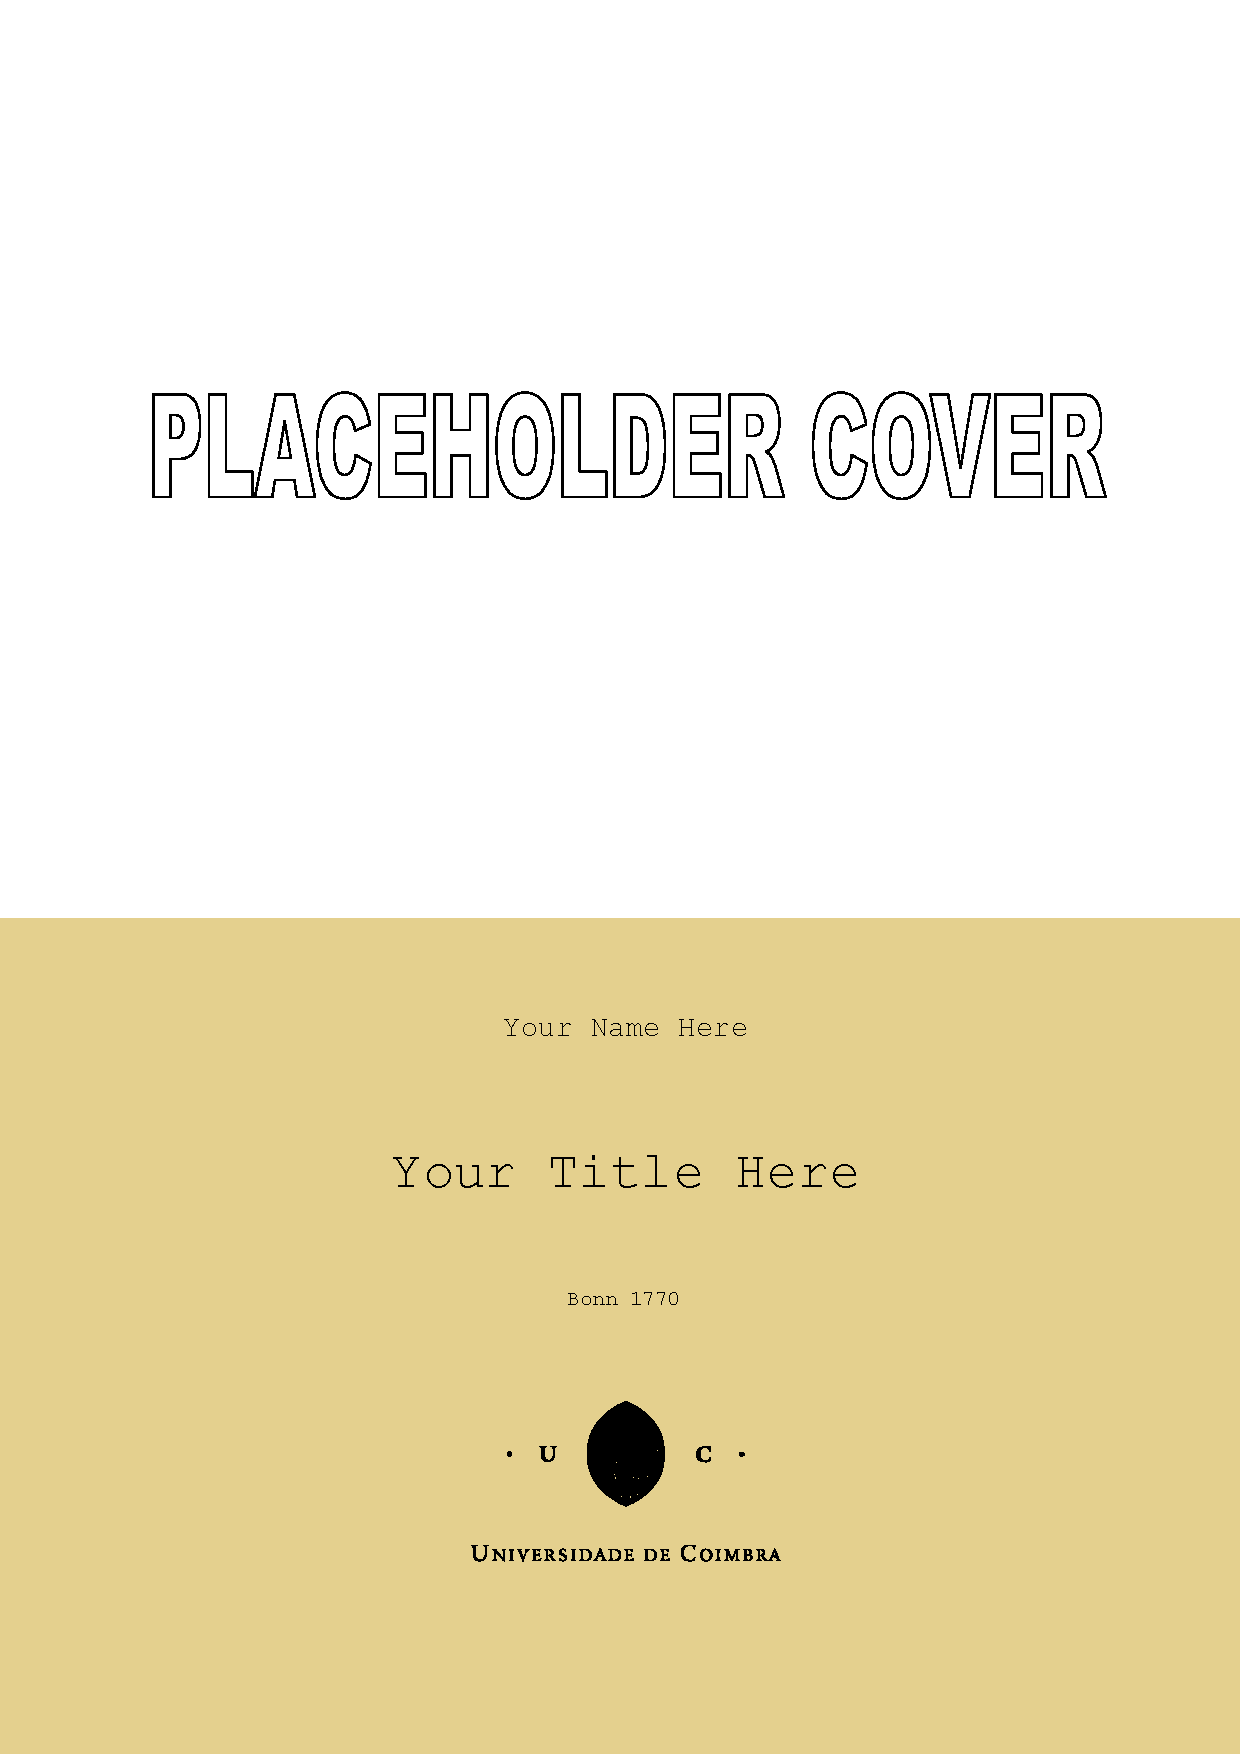
\includepdf[pages={-}]{images/cover.pdf}
% Blank page
\newpage
\thispagestyle{empty}
\mbox{}
% Title page 1
\begin{titlepage}
\thispagestyle{empty}

\begin{center}
% UC Logo and Name

\includegraphics[width=0.8\textwidth]{images/fctuc.pdf}
\par 	% Necessário, para não lixar o espaçamento
\vspace{5mm}

\includegraphics[width=0.5\textwidth]{images/fctuctext.pdf}
\par

% Thesis title
\vspace{2cm}
{\Huge{\textbf{\thesistitle}}\par}

% Your name
\vspace{2.5cm}
{\large \textbf{\myname}}

% Push stuff to bottom of the page
\vfill
{\large{\statedate}}

\end{center}
\end{titlepage}
% Blank page
\newpage
\thispagestyle{empty}
\mbox{}
% Title page 2
\begin{titlepage}
\begin{center}
% UC logo, no name

\includegraphics[width=0.8\textwidth]{images/fctuc.pdf}

% Thesis name
\vspace{1cm}
{\huge{\textbf{\thesistitle}}\par}

\vspace{1cm}
{\large{\textbf{Supervisor:}\\\supervisorname\par}}
\vspace{5mm}
{\large{\textbf{Co-Supervisor:}\\\cosupervisorname}}

\vspace{1cm}
{\large{\textbf{Jury:}

Prof. Doctor António Miguel Lino Santos Morgado

Prof. Doctor Paulo José Monteiro Peixoto 

Doctor David Bina Siassipour Portugal 

}}

% Final Stuff
\vfill
Dissertation submitted in partial fulfillment for the degree of Master of Science in Engineering Physics.

\vspace{0.5cm}
{\large \statedate\par}    


\end{center}
\end{titlepage}
% Blank page
\newpage
\thispagestyle{empty}
\mbox{}

% Acknowledgements
\chapter*{Acknowledgments}
\addcontentsline{toc}{chapter}{Acknowledgements}
% Acknowledgements
\vspace{1cm}
\noindent

During these last years, several people have been paramount for the conclusion of this thesis, and as such, I would like to acknowledge all of those who helped me in some way or another to achieve this.

First and foremost, I want to thank my family, for their love and care, who supported and helped me throughout all these years, and without whom I would never be able to continuously push forward. 

I also wish to extend my deepest gratitude to my supervisors, Prof. Mahmoud Tavakoli and in particular Dr. David Portugal, for his guidance, his continuous support, and for giving me an opportunity to undertake this challenge and so much more; I will be forever grateful.

Finally, to my closest friends, Edgar, Idálio, Daniel, Afonso, Gabriel and Brito for putting up with me all of this time, which I know to be a very troublesome task at times, and being a helping hand on this journey, thank you.
% You can add blank pages here, if you like

% ABSTRACT
\chapter*{Resumo}
\addcontentsline{toc}{chapter}{Resumo}
% Resumo em Português
\vspace{1cm}
\noindent

Nos últimos anos, em particular com o desenvolvimento da pandemia COVID-19, temos observado uma transformação digital continua dos cuidados de saúde. Uma tecnologia em específico destaca-se, revelando grande potencial para revolucionar o paradigma atual dos cuidados de saúde -- a Internet das Coisas (\acs{IoT}).

O trabalho desta dissertação consiste no desenvolvimento de uma infrastrutura \acs{IoT} que interliga sensores inteligentes vestíveis a um sistema de informação de saúde utilizado por inúmeros hospitais nacionais. 
Em particular, é efetuada uma avaliação de diferentes placas de hardware \acs{IoT} comuns para determinar que placa será utilizada para a infraestrutura de aquisição de dados, além de uma análise extensiva da comunicação Bluetooth Low Energy (\acs{BLE}) para avaliar os dispositivos utilizados para efetuar a comunicação \acs{BLE}.
No âmbito deste trabalho foi também proposta uma especificação para comunicação \acf{MQTT}, tal como o desenvolvimento de uma Interface de Programação de Aplicações (\acs{API}) usando o protocolo \acf{FHIR}, que é um dos protocolos mais utilizados para a transmissão de informação de saúde no ambiente de software clínico, para integrar a infraestrutura no sistema de informação de saúde, juntamente com uma arquitetura de serviços para o servidor \textit{edge}, desenhado com segurança e privacidade em mente.

A plataforma desenvolvida é validada através de um ensaio em instalações hospitalares e testes em ambiente controlado, nos quais a infraestrutura mostrou uso eficiente de recursos, disponibilidade máxima e boa segurança, fornecendo uma base sólida para continuar o desenvolvimento e expandir as funcionalidades existentes do sistema.

\paragraph{}\textbf{Palavras-chave:} Internet das Coisas; \acs{FHIR}; \acs{MQTT}; \acl{BLE}; Cuidados de saúde; Sensores vestíveis.

% And here

\chapter*{Abstract}
\addcontentsline{toc}{chapter}{Abstract}
% Abstract in English

\vspace{1cm}
\noindent
\textbf{} 

\todo[inline]{To-do: Add abstract text.} 

% And here as well
\newpage\null\thispagestyle{empty}\newpage

% INSPIRATIONAL QUOTE
% Setup
%\setlength\epigraphwidth{12cm}
%\setlength\epigraphrule{0pt}
%\makeatletter
%\patchcmd{\epigraph}{\@epitext{#1}}{\itshape\@epitext{#1}}{}{}
%\makeatother
% Actual Quote
%\vspace*{\fill}
%\epigraph{``Inspirational quotes are cool.”}
%{--- \textup{A renowned author}, A Great Book}
%\vspace*{\fill}
%\newpage\null\thispagestyle{empty}\newpage

% TABLE OF CONTENTS
\pagestyle{plain}
\tableofcontents

% LIST OF ACRONYMS
\chapter*{List of Acronyms}
\addcontentsline{toc}{chapter}{List of Acronyms}
\todo[inline]{To-do: Remember to check the order on the acronyms!!} 

\begin{acronym}[PROJECT\_NAME]
\acro{API}{Application Programming Interface}
\acro{BLE}{Bluetooth Low Energy}
\acro{CoAP}{Constrained Application Protocol}
\acro{ECG}{Electrocardiogram}
\acro{EHR}{Eletronic Health Record}
\acro{EPC/RFID}{EPCglobal Gen2 RFID}
\acro{FHIR}{Fast Healthcare Interoperability Resources}
\acro{HIS}{Health Information System}
\acro{IMU}{Inertial Measurement Unit}
\acro{ISR}{Institute of Systems and Robotics}
\acro{IoT}{Internet of Things}
\acro{IP}{Internet Protocol}
\acro{IT}{Information Technology}
\acro{MQTT}{Message Queuing Telemetry Transport}
\acro{MTU}{Maximum Transmission Unit}
\acro{OSI}{Open System Interconnection}
\acro{PPG}{Photoplethysmography}
\acro{RDBMS}{Relational Database Management System}
\acro{RFID}{Radio-frequency Identification}
\acro{SBC}{Single Board Computer}
\acro{SQL}{Structured Query Language}
\acro{TLS}{Transport Layer Security}
\acro{UI}{User Interface}
\acro{PHY}{Physical Layer}
\acro{ATT}{Attribute Protocol}
\acro{GATT}{General Attribute Profile}
\acro{WBAN}{Wireless Body Area Network}
\acro{JSON}{JavaScript Object Notation}
\acro{WoW}{Wireless biOmonitoring stickers and smart bed architecture: toWards Untethered Patients}
\acro{GUI}{Graphical User Interface}
\acro{PDU}{Protocol Data Unit}
\acro{SMP}{Security Manager}
\acro{ATT}{Attribute Protocol}
\acro{GATT}{Generic Attribute Protocol}
\acro{GAP}{Generic Access Profile}
\acro{DLE}{Data Length Extension}
\acro{LL}{Link Layer}
\acro{SoC}{System on a Chip}
\acro{L2CAP}{Logical Link Control and Adaptation Protocol}
\end{acronym}

% LIST OF FIGURES
\listoffigures

% LIST OF TABLES
\listoftables


% BODY
\newpage
\thispagestyle{empty}
\mbox{}
\chapter{Introduction}
\pagenumbering{arabic}	% Arabic numbering starts
%INTRODUCTION: deve responder a "WHAT?" e a "WHY?"

% This report describes the work developed under the project "Wireless IoT Architecture for Smart Nodes deployed in Hospital Beds", which took place in the Institute of Systems and Robotics (ISR) in Coimbra in the past year. 

\section{Context}

% Due to all the technological and healthcare advances over the last years, we have observed a steady increase of life expectancy. A consequence of this fact is that 

% The steadily aging population [1] and related rise of chronical illnesses places significant strain on modern healthcare systems [2]. 

% E especialmente tendo em conta a situação pandémica que vivemos, observa-se uma necessidade clara de aliviar essa pressão. Felizmente, a Internet das Coisas é vista como um grande promessa para resolver esta questão.

% Podemos hoje encontrar iniciativas que caminham nesta direção como na automatização de certos processos (como a monitorização periódica dos pacientes), aliviando a alocação de recursos, e até na área de investigação para encontrar correlações entre determinados sinais biológicos e certas patologias (também designadas de biomarcadores), permitindo efetuar diagnósticos mais rápidos e com maior facilidade.
\todo[inline]{To-do:
Steady increase of population lifespan introduces many challenges to healthcare systems (more elderly people, chronic diseases become more common, thus greater pressure on these systems, bigger healthcare costs, ...);

What has digital health done to help this? concepts: IoT, digital health...}

\section{Objectives}
\todo[inline]{To-do: Discuss if this section should move to AFTER literature review

 "Based on our previous experiences in bringing digital heath solutions to the European hospitals (see for instance the swithome project), hospitals are more likely to accept a solution, if it is already connected to their hospital information system."
}
Based on previous knowledge of digital health solutions, the main objective of this work is the development of a \acs{IoT} architecture in the context of the \acs{WoW} project. 
The system should be non-invasive, reliable and satisfy the stringent security and privacy requirements of health information systems.

\section{Thesis Structure}

This document is organized into different sections. The first chapter provides an introduction to the theme of the dissertation, discussing the context and motivation behind the work developed. In the second chapter a brief overview into \acs{IoT} systems and pervasive healthcare is shown.

%\todo[inline]{To-do: Apresentar e explicar a estrutura / organização da tese "dizer como vamos responder a "HOW?" na restante dissertação."}

% For each chapter, you should have a bit of code that looks like this:
% \label allows you to later \ref that chapter.
% \input includes a different .tex file, so that you can have you dissertation
% neatly partitioned into several files. I recommend one file per chapter.
\chapter{State of the Art}
\label{chap:stateofart}
In this chapter a survey of pervasive healthcare applications is presented. In order to gain a greater understanding of the building blocks of a typical \acf{IoT} system, a reference model for \acs{IoT} systems is also discussed. With this knowledge, we present a comparative analysis of similar works in the literature, identifying their strengths and weaknesses. The chapter is concluded by stating the contributions that this work proposes to achieve.

\section{Internet of Things}

\subsection{Fundamentals of \acs{IoT}}

% Por ser tão central ao trabalho, colocar a definição dentro de uma caixa para ficar mais realçada pode fazer sentido. Avalia isso.

\acl{IoT} (or \acs{IoT}) is an emerging communication paradigm, often hailed as the driver of the Fourth Industrial Revolution \cite{Aceto2020}. \bigskip

The definition of this concept has evolved over time with the development of other technologies such as data analytics, embedded systems, sensors, etc. Fundamentally, it can be described as the following \cite{Baker2017}: \bigskip

\todo[inline]{To-do: Find alternatives for 'strategy' - communication strategy, architecture, technology? I opted with technology, awaiting feedback}
\begin{tcolorbox}[colback=blue!5!white,colframe=blue!75!black]
    \acs{IoT} is a technology supported on the development of networks of smart devices that exchange and process information through Machine-to-Machine (M2M) communications, usually based on the \acf{IP}.
\end{tcolorbox}

This technology enables ubiquitous systems to gather remarkable amounts of information regarding the surrounding environment, which can later be turned into insight through the usage of data fusion and data analytics tools, like Machine Learning. \bigskip

In the specific context of healthcare, this technology can provide many benefits as it enables remote and continuous health monitoring \cite{Doukas2012, Wu2020, Fan2014}. It allows non-critical patients to be monitored from the comfort of their own houses, rather than in hospitals or clinics, reducing the strain on scarce hospital resources such as health professionals or beds. This is particularly beneficial to those who live in rural areas, with limited access to healthcare services. It enables elderly people and those with chronic diseases to have greater control over their own health, thus allowing them to live more independently. Moreover, with the automatization of medical procedures, these systems can make healthcare infrastructures more efficient and therefore lower the costs of healthcare \cite{Catarinucci2015, Adame2018}. Particularly, in the realm of clinical research, by analyzing the data collected by these ubiquitous systems, it may be possible to find new relationships between certain pathologies and different physiological signals, such as variations in body temperature or heart rate \cite{Choi2016}. These correlations, commonly referred to as biomarkers, can be used by these systems to assist clinical decisions, enabling novel predictive, prognostic, and diagnostic processes in healthcare.

\section{A Reference Model for Pervasive Healthcare Applications}

Reference models provide an abstract framework for designing systems and a set of commonly recommended practices for the application domain. It serves as a starting point in the design process, enabling the comprehension of complex systems by breaking them down into simple and distinct functional layers, while also defining some common terminology used in its domain. \bigskip

In 2014, the \acs{IoT} World Forum (IoTWF) architectural committee published an \acs{IoT} architectural reference model, composed by seven layers as shown in Figure \ref{fig:iotwf-referencemodel}. This model \cite{Cisco2014} provides a simple and clean functional view into the different components of an \acs{IoT} system, without narrowing the scope or locality of its components. While this model can be used to generically develop \acs{IoT} systems for any industry (\textit{e.g.} from agriculture to smart cities), in the context of the dissertation we will focus on pervasive healthcare applications. \bigskip

%\todo[inline]{To-do: Make new image based on this one. (!!)}

\begin{figure}[H]
    \centering
    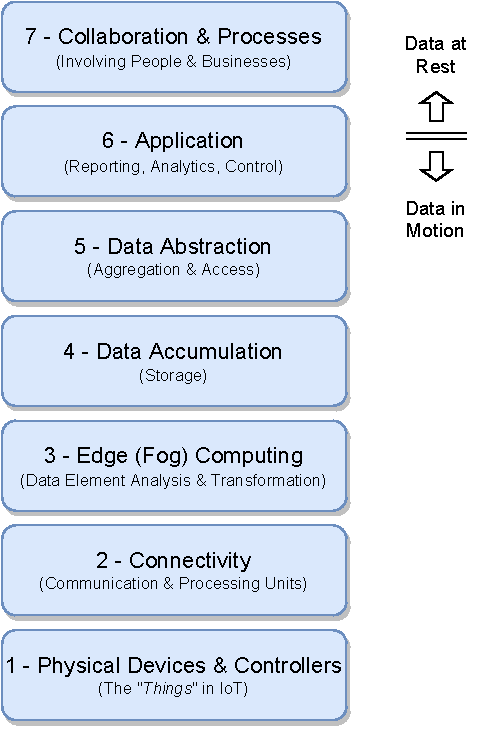
\includegraphics[width=0.6\linewidth]{images/iotwf-referencemodel.pdf}
    \caption[IoT reference model published by IoTWF.]{IoT reference model published by IoTWF. Source: \cite{Cisco2014}.}
    \label{fig:iotwf-referencemodel}
\end{figure}

From a hardware perspective, in this work we focus on the most common approach taken by researchers, using 3 distinct components: 

\begin{itemize}
    \item \textbf{Endpoint} or \textbf{edge} nodes (corresponding to Layer 1), which interact with the physical world, capturing data.
    \item \textbf{Gateway} devices (Layer 3), which connect to one or multiple \textbf{edge} nodes, filtering and aggregating the data generated by these and communicating it to a central server; 
    \item \textbf{Central} server (Layers 4-6), which is responsible for collecting, storing and analyzing the captured data in order to provide users with valuable insight;
\end{itemize}

\subsection{Layer 1: Physical Devices and Controllers}
\label{sec:iot-model-layer1}

The first layer of the model \cite{Cisco2014} corresponds to the physical devices and controller layer. This layer houses the ``things'' in the \acl{IoT}: the endpoint devices composed of sensors and actuators that perceive and interact with the physical world. Through those interactions, the devices generate data, which is then sent across the network for analysis and storage. \bigskip

Wearable, wireless, and non-intrusive devices are viewed as one of the key components of \acs{IoT}-based healthcare systems \cite{Baker2017}. In recent years there has been remarkable progress on the development of wearable devices, driven by recent technological breakthroughs in the miniaturization of sensors and microfabrication processes \cite{Adame2018, Catarinucci2015}. These devices allow patients to be monitored while retaining their mobility, increasing the comfort of these users. The drawback of this approach lies on the restrictions imposed on the devices. Due to the nature of this technology, most of these units require a portable energy source, which implies reduced memory, computation, and connectivity capabilities in order to minimize energy consumption and maximize their lifetime. Shorter lifetimes translate into higher maintenance costs, as these devices need to be replaced more often. \bigskip

Another point to consider is the data requirements of the system, namely how much data is generated and which type of data is transmitted by each device. Some applications can include a single temperature sensor or heart rate sensor, while more complex systems can include pulse oximetry, electrocardiogram (\acs{ECG}), respiration rate sensors, etc. \cite{Wu2020}. From the literature \cite{Wu2020, Wu2019, Adame2018, MinhDang2019}, the sensors used in these devices can be classified into three distinct categories based on the signals that can be extracted from them, as shown in Table \ref{tab:layer1-sensors}:

\begin{itemize}
    \item \textbf{Physiological Sensors}: used for evaluating the patients health condition.
    \item \textbf{Activity / Motion sensors}: used for detecting fall events, determining the patients location and the travelled distance, estimating the patients body posture, etc.
    \item \textbf{Environmental Sensors}: used for assessing environment conditions and possible hazards, \textit{e.g.} gas leaks in a patients home or an industrial workplace \cite{Wu2019}.
\end{itemize}

\renewcommand{\arraystretch}{2}
\begin{table}[H]
    \centering
    \begin{tabular}{l|l}
        \textbf{Sensor Categories} & \textbf{Examples} \\ 
        \hline
        Vital Signs Monitoring & \makecell{Blood Pressure, \acs{ECG}, PPG, Body Temperature, \\ Respiratory Rate, Galvanic Skin Response, \\ Pulse Oximetry, Glucose Level Sensors} \\
        Activity Monitoring & Accelerometer, Gyroscope, Magnetometer\\
        Environmental Monitoring & Air Temperature, Barometer, Humidity, Gas Sensors \\
    \end{tabular}
    \caption[Type of sensors commonly used in pervasive healthcare applications.]{Type of sensors commonly used in pervasive healthcare applications. Adapted from \cite{MinhDang2019}.}
    \label{tab:layer1-sensors} 
\end{table}
\renewcommand{\arraystretch}{1}

\subsection{Layer 2: Connectivity}
\label{sec:iot-model-layer2}

The second layer of the model focuses on connectivity, on linking the different components of the system, ensuring reliable and timely data transmissions. This includes all communications within the system, which can be divided into two categories: communications within the local network (\textit{e.g.} between edge nodes and the gateway devices), and communications between the edge of the local network (\textit{e.g.} gateway devices) and the central server. \bigskip

\subsubsection{Communication Protocols}

Technology is designed with particular use cases in mind, built to fulfill a certain need which other similar technologies fail to meet \cite{Cisco2014}. As such, each technology will be different, having advantages and disadvantages depending on its usage. For instance, short range wireless protocols are, by definition, limited by transmission range, but longer range protocols have in general a higher energy consumption, which may become unviable for networks with highly constrained devices. Some protocols communicate within certain frequency bands, some of which may require special licenses. Using licensed frequency bands can provide a better performance as it ensures greater reliability since the network operator grants you exclusivity of frequency spectrum within certain areas but may be too costly. \bigskip

From the literature, a set of key requirements that drive the decision of the communication protocols can be identified \cite{Baker2017, Catarinucci2015, Adame2018}:

\begin{itemize}
    \item \textbf{Energy consumption}: For networks composed of energy constrained devices, the communication protocol should be lightweight and energy efficient in order to maximize the devices lifetime. 
    \item \textbf{Latency}: Certain applications deal with time critical events, for example the detection of health emergencies \cite{Catarinucci2015}. In these cases, any delays in the communications can cause great detriment to the patients well-being, making it crucial to minimize them.
    \item \textbf{Reliability}: Depending on the critical nature of the data that is being communicated, the network stack may need to implement processes such as error-detection, retransmission or handshakes in the communications to ensure more robust transmissions, \textit{e.g.} as implemented in TCP/IP based protocols. Generally, these features come at the cost of greater latency. Therefore, when choosing the communication protocol, a balance must be found between reliability and latency.
    \item \textbf{Security}: Security is one of the most important requirements of any system, but this is especially true for healthcare applications. Due to the sensitive nature of the information, it is crucial to secure it from malicious actors. Communication protocols must implement security mechanisms, such as encryption or data integrity verifications, that ensure the transmissions are not compromised in transit, thus denying third parties the ability to snoop or tamper the transmissions. This issue is studied in depth in \cite{Gope2016}.
    \item \textbf{Interoperability}: To ensure the interoperability of intrinsically different modules of the system it is imperative to choose protocols that are widely accepted and supported in the application domain. This also contributes to the longevity and maintenance of the system, as these will most likely remain supported for longer time periods. 
    \item \textbf{Range}: The communication protocol must ensure that the devices can communicate within the required transmission range.
    \item \textbf{Scalability}: These systems may contain an enormous amount of devices, which must be uniquely identified. The communication protocol must ensure that every device in the network is addressable, and that performance is not severely impacted by the addition of new devices.
    \item \textbf{Throughput}: The communication protocol should ensure that there is enough bandwidth to handle all communications within the designated transmission range. Even within similar technologies, this can vary wildly with transmission range \cite{10.5555/3161403}.
\end{itemize}

% IEEE 802.15.4?
Regarding communications within the local network, these generally have short transmission ranges \cite{Baker2017}. Wearable devices can be often arranged in networks, aptly designated \acf{WBAN}. The most widely adopted protocol is \acf{BLE}, a low-energy version of the classic Bluetooth protocol \cite{Doukas2012, Wu2019, Wu2020}. ZigBee and \acf{RFID} are also used in many systems in this domain, particularly in asset tracking oriented applications \cite{Fuhrer2006, Catarinucci2015, Adame2018}. Despite the absence of a universal specification for \acs{RFID}, the most widely used standard is the EPCglobal Gen2 RFID \cite{EPCglobal2006}. For the sake of simplicity, we use \acs{EPC/RFID} to designate it. \bigskip

Out of the abovementioned technologies, \acs{BLE} offers greater throughput, better security, and nearly the lowest energy consumption \cite{dementyev2013power}. Table \ref{tab:comparsion-shortrangeprotocols} shows a comparison between the different protocols.

\renewcommand{\arraystretch}{1.5}
 \begin{table}[H]
     \centering
     \begin{adjustbox}{width=0.9\columnwidth,center}
     \begin{tabular}{r|l|l|l}
         & \textbf{\acs{BLE}} & \textbf{EPC/\acs{RFID}}& \textbf{ZigBee}  \\ \hline
         \makecell[r]{\textbf{Band of} \\ \textbf{operation}} & 2.4 GHz & LF, HF, UHF, EHF & 2.4 GHz \\
         \textbf{Communication} & Bidirectional & \makecell{Unidirectional \\ (Bidirectional for\\ Active tags)} & Bidirectional \\
         \textbf{Topology} & \makecell{ Point-to-Point, \\ Piconet, Broadcast,\\ Mesh } & Point-to-Point & Mesh \\
         \textbf{Range} & <100m & \makecell{<10m, (100m for\\ Active tags)} & 20m \\
         \makecell[r]{\textbf{Data rate} \\ \textbf{(Typical)}} & 1Mbps & 40kbps & 250kbps \\
         \textbf{\acs{IP} Stack} & \xmark & \xmark & \cmark \\
         \makecell[r]{\textbf{Security} \\ \textbf{Features}} & \makecell{AES-128, Secure \\ pairing prior to \\ key exchange} & \xmark & \makecell{AES-128 (Optional),\\ Network key shared \\across network, \\ Optional link key to \\ secure application layer \\ communications}\\
     \end{tabular}
    \end{adjustbox}
     \caption[Overview of the most common communication protocols used within short range]{Overview of the most common communication protocols used within short range. Adapted from \cite{Baker2017}.}
     \label{tab:comparsion-shortrangeprotocols}
 \end{table} 
\renewcommand{\arraystretch}{1}

Regarding communications between the gateway devices and the central server, most researchers try to make use of existing infrastructure in order to facilitate the deployment of new systems. This means, that the communications between the gateway devices and the central server are often done through generic IP-based protocols such as Wi-Fi and Ethernet \cite{Adame2018, Fuhrer2006, Wu2020, Catarinucci2015}. \bigskip

\subsubsection{Application Protocols}
%\todo[inline]{To-do: Remake this intro paragraph?}

So far we have discussed the underlying networking technologies that link the devices in system. But according to the OSI Model, many of these technologies do not define the application layer: how the devices communicate with each other, how the data is formatted, if there is a hierarchy within the network, etc. When considering networks composed of constrained devices, generic web-based protocols such as Hypertext Transfer Protocol (HTTP) may not be adequate for \acs{IoT} applications, which prompts the development of novel lightweight messaging protocols suited for these systems. The most used application layer protocols in \acs{IoT} systems are \acf{MQTT} and \acf{CoAP}. Table \ref{tab:comparsion-applicationprotocols} overviews these widely used protocols. \bigskip

\renewcommand{\arraystretch}{1.5}
\begin{table}[H]
    \centering
    \begin{tabular}{r|l|l}
        %\textbf{Features} 
        & \textbf{\acs{MQTT}}& \textbf{\acs{CoAP}}  \\ \hline
        \textbf{Transport protocol} & TCP/IP & UDP/IP \\
        \textbf{Messaging pattern} & \makecell{Publish/Subscribe \\ (asynchronous)} & \makecell{Request-Response \\ (synchronous)} \\
        \textbf{Communication model} & Many-to-many & One-to-one \\
        \textbf{Security} & SSL/TLS (Optional) & DTLS \\
        \textbf{Strengths} & \makecell{TCP and Quality of \\ Service (QoS), robust \\communications, easier \\ to implement } & \makecell{Better for lossy networks,\\ lower latency} \\
        \textbf{Weaknesses} & \makecell{Higher overhead and energy\\ consumption than \acs{CoAP}} & \makecell{Not as reliable and \\less supported than MQTT} \\
    \end{tabular}
    \caption[Comparison between \acs{CoAP} and \acs{MQTT} protocols.]{Comparison between \acs{CoAP} and \acs{MQTT} protocols. Adapted from \cite{10.5555/3161403}.}
    \label{tab:comparsion-applicationprotocols}
\end{table} 
\renewcommand{\arraystretch}{1}

In \cite{Rubi2019}, the authors compare these two protocols in greater length, along with the more commonly used web-based protocol Hypertext Transfer Protocol (HTTP). They analyze the latency in the communications (from the edge devices to remote servers) and the RAM usage in the devices for each protocol and for different data sources (respiration rate, oxygen saturation and heart rate signals) and found that \acs{CoAP} presented the best overall performance. Nonetheless, all protocols had very low latencies (less than 1.5s) and low memory usage.

\paragraph{} The authors indicate that \acs{MQTT} might be more suitable when considering a certain messaging pattern — the ``Publish/Subscribe'' model. In this model, the devices that send messages, called ``publishers'', communicate them to an intermediary message broker, through a ``message topic'' (also called logical channels). The devices that wish to receive messages, called ``subscribers'', can subscribe to these topics by requesting it to the message broker. Whenever a publisher sends a message, the broker broadcasts it to all devices that have subscribed to the selected topic.

\paragraph{} \acs{CoAP} uses a different messaging pattern, called ``Request-Response''. In this paradigm, a device sends a request to receive certain data and the second responds to this request.
 % observe that the former model is event-driven while the latter is query-based \cite{Rubi2019}. % Due to the nature of how the data is generated in these types of pervasive applications, an event-driven protocol like \acs{MQTT} might be more adequate.

\begin{figure}[H]
    \centering
    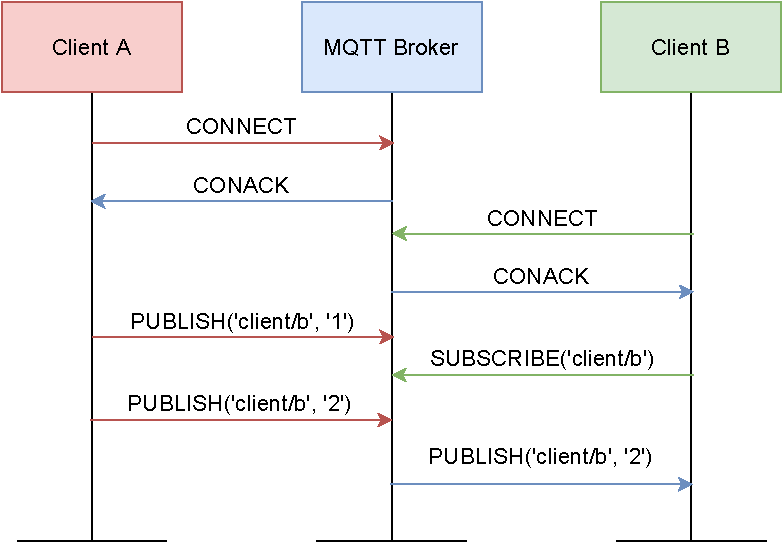
\includegraphics[width=0.75\linewidth]{images/mqtt message sequence diagram.pdf}
    \caption[Diagram of a \acs{MQTT} message sequence.]{Diagram of a \acs{MQTT} message sequence. In this diagram, we have two clients (A and B) connecting to the \acs{MQTT} broker, where client A transmits two messages to the topic ``client/b'' while client B subscribes to that topic to demonstrate how the Publish-Subscribe model works. In \acs{MQTT}, a client recieves a message whenever a client (including itself) publishes a message on that topic.}
    \label{fig:mqtt-message-sequence-diagram}
\end{figure}

\begin{figure}[H]
    \centering
    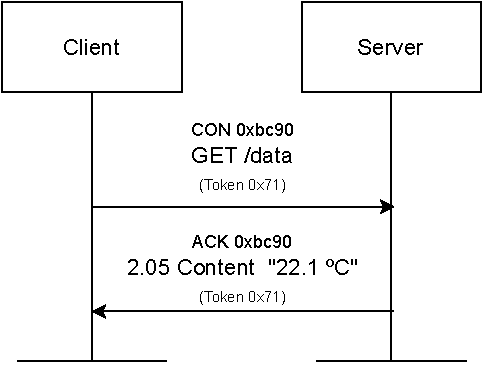
\includegraphics[width=0.5\linewidth]{images/coap message sequence diagram.pdf}
    \caption[Diagram of a \acs{CoAP} message sequence.]{Diagram of a \acs{CoAP} message sequence. In this diagram, we have a client making a GET request to the \acs{CoAP} server to retrieve information, in order to demonstrate how the Request-Response model works. In \acs{CoAP}, the requests are delivered asyncronously, and so the response messages must contain a ``token'' value so that the client can identify which request resulted in this response.}
    \label{fig:coap-message-sequence-diagram}
\end{figure}

\subsection{Layer 3: Edge (Fog) Computing}
\label{sec:iot-model-layer3}

\acs{IoT} systems may have hundreds or even thousands of sensors generating data multiple times per second, 24 hours per day, which may require an unsustainable amount of network and computing resources. Moreover, certain applications are time critical, where delays in communication can be very detrimental. To minimize these effects, it is crucial to initiate data processing as close to the edge of the network as possible. This paradigm is usually referred to as edge computing, when the data processing occurs at the endpoint devices, or fog computing, when it happens at the edge of the local network, \textit{e.g.} in gateway devices. \bigskip

The third layer of the model defines how the system prepares the data for storage and higher level processing for the next layers. However, the endpoint or gateway devices often have limited computing capabilities, so the data processing is generally focused on preprocessing the data in real-time and handling more time critical events. More demanding and thorough data analysis is usually left to the central server. \bigskip

The different processes applied at this stage can be summarized into four distinct categories:

\begin{itemize}
    \item \textbf{Filtering}: Assessing if the data should be processed at a higher level. 
    \item \textbf{Formatting}: Reformatting data to ensure consistent formats for higher-level processing.
    \item \textbf{Cleaning}: Reducing data to minimize the impact of data on the network and higher level processing systems.
    \item \textbf{Evaluation}: Determining whether data represents a threshold or alert. This is especially relevant for applications that deal with time critical events as seen in the previous section.
\end{itemize}

% \todo[inline]{To-do: Add 2 examples of edge computing processes discussed in the systems?} 

\subsection{Layer 4: Data Accumulation}
\label{sec:iot-model-layer4}

The data that is generated by the edge devices is propagated through the system, and eventually reaches the central server. Up to this point, the model is event driven. However, most applications cannot make use of the data at the rate it is generated \cite{10.5555/3161403}. In the Data Accumulation layer, we need to define how the system captures the data and stores it, so it becomes usable for applications when needed, thus transiting from event to query-based processing. \bigskip

As the devices continuously generate data, the system will require more and more resources in order to process and store all of this information, raising some concerns regarding how the data can be managed. In \cite{Doukas2012}, the authors propose the usage of cloud platforms as a solution to these problems. This is made possible due to the elasticity in allocating, swiftly and inexpensively, computing and storage resources on-demand, adjusting itself to the needs of each application. We can identify three distinct types of cloud services: 

\begin{itemize}
    \item \textbf{Infrastructure as Service (IaaS)}: Provides control over the remote machine (composed of virtual or dedicated hardware), operative system and middleware. This approach gives system designers the highest level of flexibility over the infrastructure, but requires more maintenance.
    \item \textbf{Platform as a Service (PaaS)}: Provides a simple framework for developing applications, where the service provider manages the underlying infrastructure issues such as software updates and hardware maintenance. 
    \item \textbf{Software as a Service (SaaS)}: Provides the finished applications to be used by the end users, in this case health workers, that enable them to work. A simple example is a web-based email service, such as Gmail or Microsoft Outlook. 
\end{itemize}

\begin{figure}[H]
    \centering
    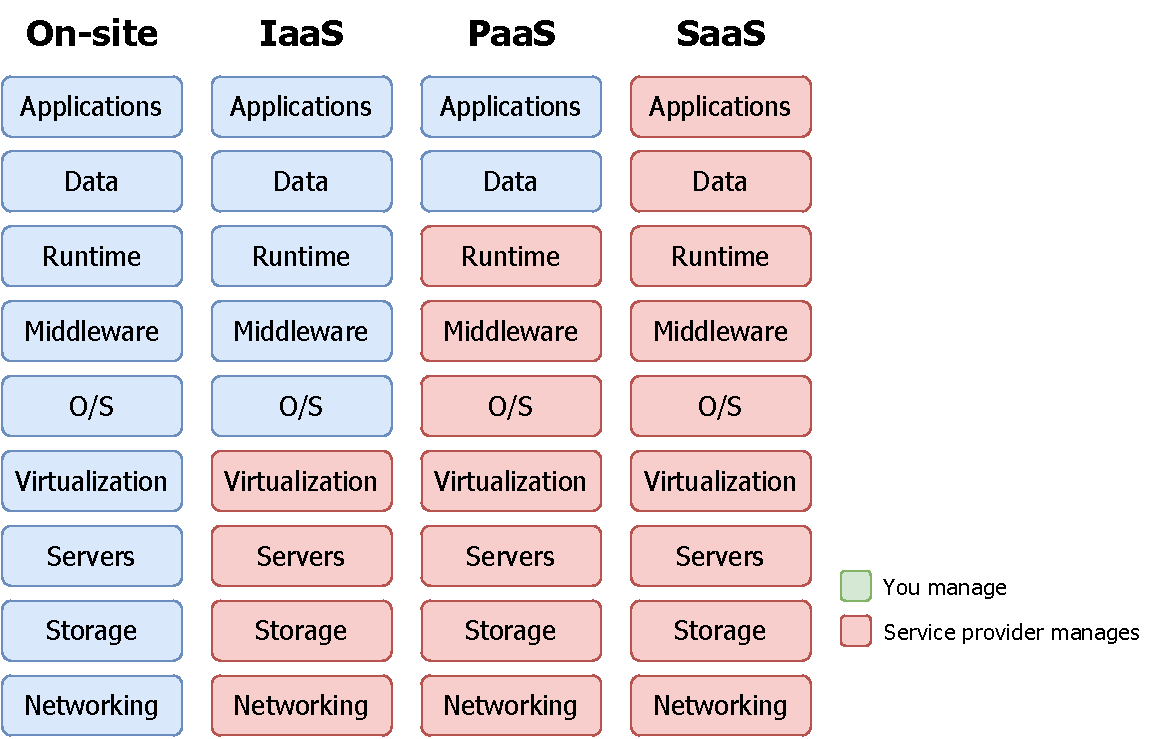
\includegraphics[width=0.85\linewidth]{images/cloud-services.pdf}
    \caption[Differences between the cloud offerings and on-premise solutions.]{ Differences between the cloud offerings and on-premise solutions. Source: \cite{RedHat2021}}
    \label{fig:differences-between-cloud-services}
\end{figure}

% \todo[inline]{To-do: Should homomorphic encryption methods be discussed? Discuss what is Hadoop? What are the 5 Vs of Big Data?}

Nonetheless, security and privacy remain as key concerns for the implementation of cloud-based solutions. The information must remain accessible to authorized parties such as healthcare providers, but the patients health data has to be kept private. To solve this, there are two commonly adopted features in the literature: access control policies and data encryption \cite{Baker2017}. Access control policies define who can access the data, by authenticating them (validating the identity of the user) and by authorizing them (ensuring that the user has permissions to perform a given operation). Data encryption ensures that, even if the data is leaked, it is still unreadable to third parties, and therefore sensitive information remains secure and private. \bigskip

Regarding storage solutions, most research works use traditional relational databases (RDBMS) as the means of storing data \cite{Fuhrer2006, Wu2020, Catarinucci2015, Adame2018}. These are often referred to simply \acs{SQL} or \acf{SQL} databases, which is the language used to interact with the database.

However, since the data in \acs{IoT} can very heterogenous and unstructured, the authors of \cite{Subahi2019} propose using NoSQL databases. NoSQL or ``not only SQL'' describes a class of database systems that can support -- and are more optimized for -- storing semi-structured and unstructured data. NoSQL data stores typically outperform SQL databases as the data increases in volume \cite{Xu2014}. Table \ref{tab:comparsion-databasetech} illustrates the differences between these two technologies. 

\renewcommand{\arraystretch}{2}
\begin{table}[H]
    \centering
    \begin{adjustbox}{width=0.9\columnwidth,center}
    \begin{tabular}{r|l|l}
        %\textbf{Features} 
        & \textbf{SQL}& \textbf{NoSQL}  \\ \hline
        \textbf{Type of database} & Relational & Non-relational \\
        \textbf{Database model} & Table-based database & \makecell{Document-based databases, \\ Key-value stores, graph stores, \\ wide column stores} \\
        \textbf{Data type} & Appropriate for structured data & \makecell{Appropriate for unstructured or \\ semi-structured data} \\ 
        \textbf{Schema} & Strict schema & Dynamic schema \\
        \textbf{Query} & \makecell{Uses Standard Query \\Language (SQL), appropriate for \\ complex query operations} & \makecell{No standard query language}  \\ 
        \textbf{Scalability} & Vertical & Horizontal \\
        \textbf{Performance} & \makecell{Generally lower than \\ NoSQL systems} & Optimized for large datasets \\
    \end{tabular}
    \end{adjustbox}
    \caption{Comparison between SQL and NoSQL database technologies.}
    \label{tab:comparsion-databasetech}
\end{table} 
\renewcommand{\arraystretch}{1}

\subsection{Layer 5: Data Abstraction}
\label{sec:iot-model-layer5}

%\todo[inline]{To-do: Complete section (develop FHIR section).} 

In the previous layer, we have defined how the system captures the information. In some cases, the collection of data may require the development of multiple concurrent storage solutions, each using different technologies, resulting in a very complex environment. The purpose of this layer is to develop services that simplify how the applications access the data, to reconcile the different data stores and ensure the information is complete and consistent \cite{Cisco2014}. Applications can then interact with these databases through interfaces exposed by these services, designated \acl{API}s (\acs{API}s). \bigskip 

An \acs{API} is a computing interface that defines a set of rules that ``explain how computers and applications communicate with one another'', acting as an intermediary between these different components \cite{IBMAPI}. It defines which operations can be performed, how to request them, which are the accepted data types, etc. In this case, it decouples applications from the storage solutions, by encapsulating their functionality behind the interface. This ensures the modularity of the system as the applications become independent of whichever technologies are used in the data stores. \bigskip

Understanding what and how information is shared within the healthcare domain is fundamental. As patients continuously circulate through the healthcare ecosystem, their health information must be available, discoverable and understandable to different entities (hospitals, laboratories, pharmacies, etc.). This prompts the digitization of medical files and the development of standards for exchanging these records instantly and securely to authorized parties \cite{HL72019}, which are called \acl{EHR}s (\acs{EHR}s). \acs{EHR}s are the digital equivalent of a patient's paper-chart, they contain the patient's full medical history: previous diagnoses, treatment plans, test results, known allergies, among other details. \bigskip

One of the most prominent standards for exchanging \acs{EHR}s is \acf{FHIR}. \acs{FHIR} is a standard developed by Health Level Seven International (HL7), which is a non-profit organization involved in the development of international healthcare informatics for over 20 years. \acs{FHIR} builds upon previous data format standards like HL7 v2 and HL7 v3, and is becoming widely adopted within the healthcare industry \cite{Peng2019}. This standard defines a lightweight RESTful framework using common data formats, like JSON and XML, so it can be readily integrated into lightweight web services, thus underlining its suitability for web-based platforms \cite{Gruendner2019}.

% \todo[inline]{To-do: If time allows it, add 2 examples of articles where APIs implemented.} 

\subsection{Layer 6: Application}
\label{sec:iot-model-layer6}

The sixth layer corresponds to the application layer, where the system ingests the captured data, analyzes it and delivers the value to the end users. Users can then interact with the system through \acl{UI}s (\acs{UI}s), which provide different functionalities depending on the application. Some may show simple reports regarding the collected data \cite{Doukas2012, Wu2020}, and others may allow users to monitor and have greater control over the different components of the system. \bigskip

As seen in an earlier section, Table \ref{tab:layer1-sensors} shows what kind of information is generally acquired in \acs{IoT} healthcare applications. Using artificial intelligence, it is also possible to correlate all of this information to guide the clinical decisions from healthcare providers \cite{Gruendner2019, Wagholikar2017, Raposo2021}. \bigskip
\subsection{Layer 7: Collaboration and Processes}
\label{sec:iot-model-layer7}

% Não removia, uma secção curta e concisa está OK porque não é tão relevante para o trabalho como as outras.
% Podes mencionar, de forma conceptual apenas (não estou a ver nesta fase como operacionalizar no projecto ainda, nem vala a pena especular) o seguinte:
% "Analyze opportunities to improve the efficiency and effectiveness of the processes."
% "Identification of the goals, deliverables, activities, patterns of collaboration, techniques, actions, and technologies associated with each process."
% Ver:
% https://ieeexplore.ieee.org/document/6148656


The information that is created by the \acs{IoT} systems yields little value unless it prompts action, which requires integrating people and business processes (seventh layer). The purpose of these systems is to empower people to work better and more efficiently by providing valuable insight at the right time. To do this, people must be able to communicate and collaborate, which often requires multiple steps and transcends multiple applications \cite{Cisco2014}. However, this component of the system is beyond the scope of this work and thus it is not discussed further.

\section{Survey on \acs{IoT} Applications for Healthcare}
\label{sec:sim-approaches}
% \todo[inline]{To-do: Complete section!  Add introductory paragraph!  Perform a critical analysis of all related work. You should make clear and focus on what is your contributions, and state clearly what is *not* your contributions (i.e. out of the scope of this work). Falta um parágrafo introdutório. O que se vai fazer nesta sub.secção? pq }

% This chapter presents a survey of patrolling, surveillance, navigation and exploration strategies already implemented in the literature. In the last decades, related algorithms for multiple robot teams have piqued the interest of the robotics community, becoming a remarkable growing area. One of the main reasons contributing to this fact is the variety of approaches that these algorithms can comprise. Many authors contributed with studies that involve many different strategies to solve these problems. In this section, some of the background work related to different strategies is presented. The reader will note that it is not imperative to follow just one of these strategies. In fact, most of them result from mixed strategies, though more evident characteristics related to the strategy being discussed are focused in each section.
% <---- Real-time tracking systems ---->

We have thoroughly discussed how \acs{IoT} systems are designed, but so far we have not discussed details of any specific implementation so far. This section presents an overview of \acs{IoT} connected healthcare applications described in the literature, highlighting each of their strengths and weaknesses. \bigskip
%==========================================================================================================================================
%[1] P. Fuhrer and D. Guinard, “Building a smart hospital using RFID technologies,” Eur. Conf. eHealth 2006, Proc. ECEH 2006, pp. 131–142, 2006.
%
%--------------------------
% Physiological & Environmental Signals: (L1) 
% - RFID tag
% Networking Protocols: (L2)
% - RFID (EPC Gen1?), WiFi
% Gateway: (L3)
% - Beaglebone Black
% Data Storage: (L4)
% - MySQL
% e-Health Standards: (L5)
% - None
% Application Features: (L6)
% - Real-Time Tracking System (Patients and Assets)
% Security:
% - Unknown Storage Encryption 
% User Interface:
% - Custom Web application
% Other Notes: 
%------------------------------

In \cite{Fuhrer2006}, one of the first \acs{IoT} applications for healthcare is described. The authors propose a real-time locating system (RTLS) using \acs{RFID} tags called RFIDLocator. These tags are placed in hospital equipment, staff, patients and medical files and by using \acs{RFID} readers placed in strategic locations around the hospital (\textit{e.g.} entrance of rooms, handheld readers), it is possible to track the location of each object. When a \acs{RFID} reader detects a \acs{RFID} tag it communicates this information, using Wi-Fi, to a central server which stores it in a MySQL database. Healthcare workers can then view this information through a web application, which contains a location history of the tagged object. The authors show how RTLS systems can mitigate the risks of patient misidentification, loss or theft of assets and even drug counterfeiting. However, in this article, security and privacy issues are not discussed. Although not stated explicitly, communications between the RFID tags and the RFID readers are assumed to be unencrypted, which means ``unethical individuals could snoop on people and surreptitiously collect data (...) without their knowledge'', even after leaving the hospital if the tags are not removed. This raises serious privacy concerns, as the tags could contain private information that can be detrimental to the patients if revealed. \bigskip

%==========================================================================================================================================
%[2] T. Adame, A. Bel, A. Carreras, J. Melià-Seguí, M. Oliver, and R. Pous, “CUIDATS: An RFID–WSN hybrid %monitoring system for smart health care environments,” Futur. Gener. Comput. Syst., vol. 78, pp. %602–615, Jan. 2018, doi: 10.1016/j.future.2016.12.023.
% 
%--------------------------
% Physiological & Environmental Signals: (L1) 
% - Temperature, Heart Rate, Accelerometer
% Networking Protocols: (L2)
% - RFID (European UHF EPC Gen2), WiFi
% Gateway: (L3)
% - Beaglebone Black
% Data Storage: (L4)
% - MySQL
% e-Health Standards: (L5)
% - None
% Application Features: (L6)
% - Real-Time Tracking System (Patients and Assets), Fall Detection, Vital signs monitoring 
% Security:
% - AES-128 (iot node <-> gateway), WPA-Personal (gateway <-> server)
% User Interface:
% - Custom Web application
% Other Notes: 
% - Ran a hospital trial
%------------------------------

In \cite{Adame2018}, the authors propose a RTLS system that also monitors the patient's vital signs, using a small wristband which holds a low power device equipped with temperature, photoplethysmography (\acs{PPG}), used to obtain the heart rate, and accelerometer sensors, used for detecting fall events. The system can also detect with 70\% accuracy if the patient has fallen, sending an immediate message to the gateway, which will later alert the clinical staff to the emergency. The authors ran a pilot test within hospital premises which was well-received by the clinical staff who praised the system for its intuitiveness and non-intrusiveness, stating that it could be easily integrated into their current \acs{HIS}. However, the authors pointed out some issues related to the usage of \acs{RFID} tags with sensors for patient monitoring. The \acs{RFID} reader powers the \acs{RFID} tags, and when using tags with sensors, the readers need to provide considerably more energy to the tags. The readers must be adjusted to provide enough power, but local regulations limit the transmission power. Regarding e-health standards, the authors did not discuss any protocols for exchanging data such as \acs{FHIR}, which can undermine the integration of the system with existing \acs{HIS}s. \bigskip

%==========================================================================================================================================
%[3] L. Catarinucci et al., “An IoT-Aware Architecture for Smart Healthcare Systems,” IEEE %Internet Things J., vol. 2, no. 6, pp. 515–526, Dec. 2015, doi: 10.1109/JIOT.2015.2417684.
%
%--------------------------
% Physiological & Environmental Signals: (L1) 
% - Temperature, ECG, Accelerometer, Barometric Pressure, Ambient Light
% Networking Protocols: (L2)
% - RFID (European UHF EPC Gen2), 6LowPAN
% Gateway: (L3)
% - TI MSP430F2618, Smartphone
% Data Storage: (L4)
% - 
% e-Health Standards: (L5)
% - None
% Application Features: (L6)
% - Real-Time Tracking System (Patients and Assets), Fall Detection, Vital signs monitoring 
% Security:
% - 
% User Interface:
% - 
% Other Notes: 
% - 
%------------------------------
% \cite{Catarinucci2015}

%==========================================================================================================================================
%[4] T. Wu, F. Wu, C. Qiu, J. M. Redoute, and M. R. Yuce, “A Rigid-Flex Wearable Health Monitoring Sensor Patch for IoT-Connected Healthcare Applications,” IEEE Internet Things J., vol. 7, no. 8, pp. 6932–6945, 2020, doi: 10.1109/JIOT.2020.2977164.
%
%
%--------------------------
% Measured Signals: (L1) 
% - 
% Networking Protocols: (L2)
% - BLE (v4)
% Gateway: (L3)
% - Raspberry Pi 3, Smartphone
% Data Storage: (L4)
% - MySQL
% Data Formats: (L5)
% - 
% Application Features: (L6)
% - 
% Security:
% - AES-128
% Integration with HIS:
% - No
% Other Notes: 
% - 
%------------------------------
%Future Work:
%"Since security is not the focus of this article, the two common security measures are implemented to meet the basic requirements of the following: (...) Security Between Wearable Patches and Gateways (...) Security Measures in Gateways and Cloud Server"
%"In our future work, more edge computing functions on the gateway will be developed for an IoT-connected healthcare platform."

%\todo[inline]{To-do: Review the critical analysis of this article.}

Wu et al. \cite{Wu2020} have developed a system which uses wearable sensor patches to monitor the patients' status. The wearable sensors transmit the different physiological signals (\acs{ECG}, \acs{PPG} and body temperature) to gateways using \acs{BLE}, which can either by fixed (using a Raspberry Pi module) or mobile (using a smartphone app). The gateway exchanges data with the cloud through bridged \acs{MQTT} brokers, after which it is stored in a MySQL database. The data is stored both in the cloud server and in the fixed gateway. The local users can interact with the system through a web-based user interface (UI) using the smartphone or other web browsers in the local area network. However, the usage of local data storage can cause data integrity issues as the system must ensure databases in both the server and gateways are synchronized at all times. This can undermine the scalability of the system, as the redundant data synchronization can become a performance bottleneck in the long term. \bigskip

%==========================================================================================================================================
%[5] C. Doukas and I. Maglogiannis, “Bringing IoT and Cloud Computing towards Pervasive Healthcare,” in 2012 Sixth International Conference on Innovative Mobile and Internet Services in Ubiquitous Computing, Jul. 2012, pp. 922–926, doi: 10.1109/IMIS.2012.26.
%
%
%--------------------------
% Measured Signals: (L1) 
% - 
% Networking Protocols: (L2)
% - BLE (v4)
% Gateway: (L3)
% - Smartphone
% Data Storage: (L4)
% - MySQL
% Data Formats: (L5)
% - Unknown
% Application Features: (L6)
% - 
% Security:
% - AES-128
% Integration with HIS:
% - No
% Other Notes: 
% - 
%------------------------------

In \cite{Doukas2012}, the authors proposed a \acs{IoT} infrastructure that acquires real-time patient data from wearable sensors, using a cloud platform to handle all data processing and storage requirements. The authors have developed a wearable device which takes the form of a sock, designated ``CloudSensorSock''. The CloudSensorSock acquires mobile data, through accelerometer and gyroscope sensors, vital data, through temperature and heartbeat sensors, and contextual information about the patient's environment using air quality ($CO_2$) sensors. It communicates with a mobile app through \acs{BLE}, which acts as a gateway to the cloud server. The authors propose moving the data processing entirely to the cloud server as cloud platforms can scale to the needs of the application with little management and cost. However, this approach may not be viable for time critical applications. As discussed earlier, the latency in the communications between devices and remote servers may have a negative impact on the application, especially since the authors propose using this system for detecting fall events. \bigskip

%==========================================================================================================================================
%[6] eCovig
%
%
%--------------------------
% Measured Signals: (L1) 
% - 
% Networking Protocols: (L2)
% - BLE (v4)
% Gateway: (L3)
% - Smartphone
% Data Storage: (L4)
% - Unknown
% Data Formats: (L5)
% - 
% Application Features: (L6)
% - 
% Security:
% - Unknown
% Integration with HIS:
% - No
% Other Notes: 
% - 
%------------------------------

Recently, and motivated by the COVID-19 pandemic, Raposo et al. \cite{Raposo2021} developed a system called ``e-CoVig'' a low-cost solution for monitoring COVID-19 patients during the quarantine, as shown in Figure \ref{fig:ecovig-architecture}. The data acquisition is performed using a mobile app. To collect physiological data, the authors developed a specialized wearable device that communicates with the mobile app through \acs{BLE}, recording pulse oximetry ($SpO_2$), heart rate, and temperature data. Alternatively, patients can use their own measuring devices, \textit{e.g.} a thermometer, and manually insert the measurements or use Optical Character Recognition (OCR) to automate the in-app insertion of the values. The app can also be used to record audio snippets in order to detect cough and monitor respiratory activity. Unfortunately, the lack of e-health standards hinders its integration with external healthcare systems. 

\begin{figure}[H]
    \centering
    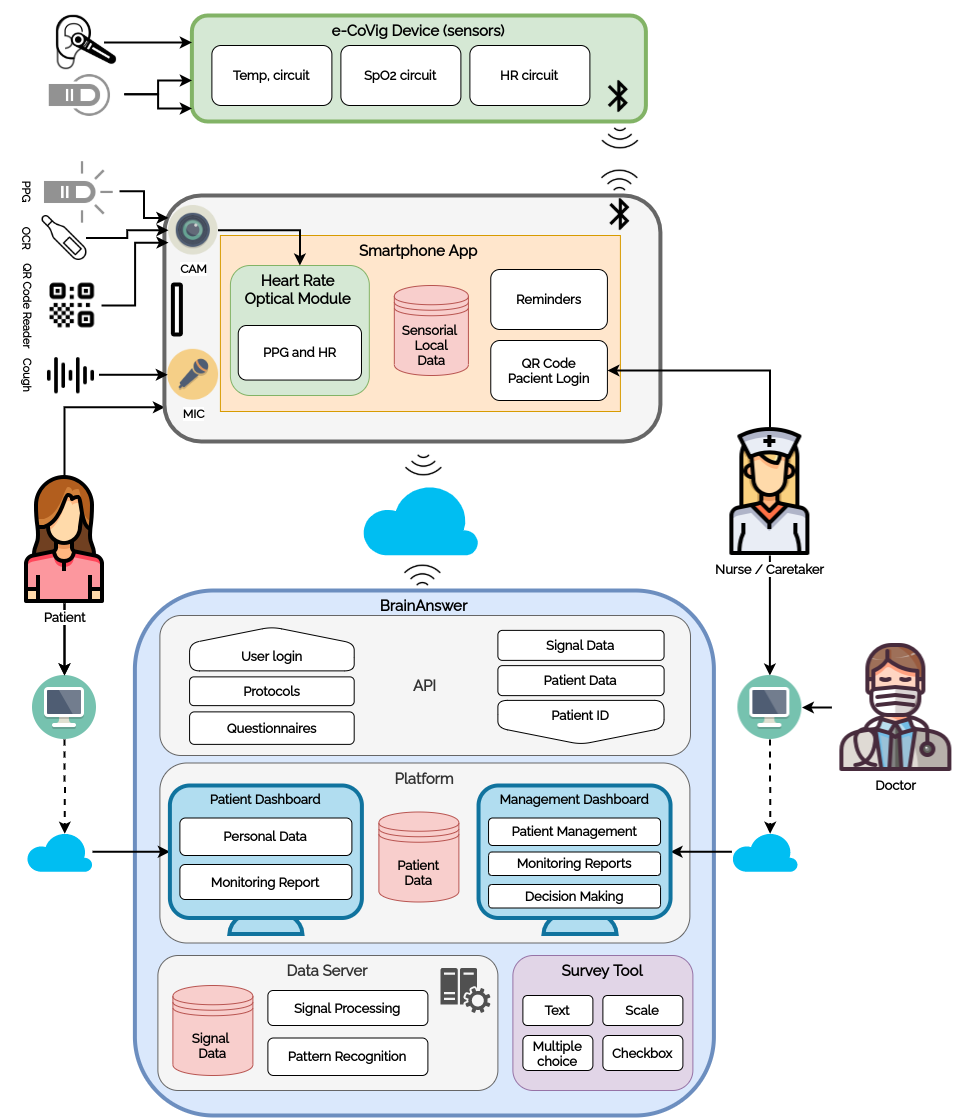
\includegraphics[width=0.60\linewidth]{images/ecovig.png}
    \caption[Diagram of e-Covig's system architecture.]{Overview of e-Covig's system architecture. Source: \cite{Raposo2021}.}
    \label{fig:ecovig-architecture}
\end{figure}


In order to summarize the key properties of the previously discussed solutions, the following table, Table \ref{tab:comparsion-articles} is presented.

\begin{landscape}
\renewcommand{\arraystretch}{2}
\begin{table}[h]
    \centering
    \begin{adjustbox}{width=\columnwidth,center}
    \begin{tabular}{l|l|l|l|l|l|l}
      \textbf{References} & \makecell{\textbf{Measured} \textbf{Signals}} & \makecell{\textbf{Networking} \textbf{Protocols}}& \makecell{\textbf{Data} \textbf{Storage}} & \makecell{\textbf{e-Health} \textbf{Standards}} & \makecell{\textbf{Application} \\ \textbf{Features}} & \textbf{Security Features} \\ \hline
        Fuhrer et al. \cite{Fuhrer2006} & N/A & \makecell{EPC/RFID,\\ Wi-Fi} & MySQL & None & \makecell{RTLS}& \makecell{Unspecified Storage \\Encryption} \\ \hdashline
        Adame et al. \cite{Adame2018} & \makecell{Temperature, \\Heart Rate,\\ Accelerometer} & \makecell{EPC/RFID,\\ Wi-Fi} & MySQL & None & \makecell{RTLS, \\ Fall Detection,\\ Vital signs\\ monitoring}& \makecell{AES-128, WPA-Personal} \\ \hdashline
        %\cite{Catarinucci2015} & \makecell{Temperature, \\ \acs{ECG}, Accelerometer,\\  Barometric Pressure,\\  Ambient Light} & \makecell{EPC/RFID, 6LowPAN,\\ CoAP} & MySQL & None & RTLS & ? \\
        Wu et al. \cite{Wu2020} & \makecell{Temperature, \\Heart Rate,\\ Accelerometer} & \makecell{BLE, Wi-Fi, \\ MQTT} & MySQL & None & \makecell{RTLS, \\ Fall Detection,\\ Vital signs\\ monitoring}& \makecell{AES-128} \\ \hdashline
        Doukas et al. \cite{Doukas2012} & \makecell{Temperature, \\Heart Rate,\\ Accelerometer, \\$CO_2$ Sensor} & \makecell{\acs{BLE}, Wi-Fi, GPRS/3G \\ HTTP} & MySQL & None & \makecell{Fall Detection, \\ Vital signs \\ monitoring} & AES \\ \hdashline
        Raposo et al. \cite{Raposo2021} & \makecell{Temperature, \\Heart Rate,\\ Pulse Oximetry, \\ Respiration Rate } & \makecell{\acs{BLE} Wi-Fi} & Unknown & None & \makecell{Fall Detection,\\ Vital signs\\ monitoring, \\ Clinical decision\\  support } & Unknown \\ 
        %\cite{} & & & & & &  \\
      \end{tabular}
    \end{adjustbox}
    \caption{Comparison between different pervasive healthcare applications.}
    \label{tab:comparsion-articles}
\end{table} 
\renewcommand{\arraystretch}{1}
\end{landscape}
\clearpage
\subsection{Weaknesses of literature}
\label{sec:weaknesses}

% Apenas identificas o problema da Interoperabilidade e Standards?
% Pensa tb nas questões de segurança e escalabilidade. 
% Pode não ser uma fraqueza/desafio comum a *todos* os trabalhos na literatura mas ser algo q nem sempre é bem resolvido.

From the literature, we find that many solutions secure communications between the devices using standard encryption algorithms like Advanced Encryption Standard (AES) \cite{Adame2018, Wu2020, Doukas2012}. However, very few discuss authentication and authorization processes \cite{Doukas2012, Gope2016}. To ensure that no data is leaked to malicious authors, the networking protocols used must ensure these \textbf{security} properties. \bigskip

Several web services currently use \acf{TLS}\footnote{The Transport Layer Security (TLS) Protocol Version 1.3: https://tools.ietf.org/html/rfc8446}. This protocol ensures integrity, confidentiality and authentication as it combines public key cryptography to validate the identity of the communicating parties, symmetric-key algorithms to encrypt the transmissions and message integrity checks to ensure the transmissions are not tampered during transport. These properties make this protocol invaluable for secure communications over the web, and thus should be an integral component of \acs{IoT} networks. Moreover, access control needs to be considered. Systems are composed by many devices, which may have different levels of access level for each device. For example, limiting access to certain topics in \acs{MQTT}, so that devices can only subscribe and publish messages in specific topics.        
 
Despite recent efforts, \textbf{interoperability} is still an issue for \acs{IoT} systems. Due to the lack of clear and concise industry standards and regulations, many manufacturers develop their own proprietary data formats and communication protocols, which hampers the integration of new resources since solutions are designed within closed ecosystems \cite{Rubi2019}. \bigskip

Fortunately, there are several international initiatives to promote the use of \acs{IoT} in health in a standardized way, such as HIMSS (Healthcare Information and Management Systems Society) and the Personal Connected Health Alliance (PCHAlliance). PCHAlliance, for example, advocates the adoption of the Continua Design Guidelines (CDG), which facilitates the integration of personal health devices into health systems. These guidelines have been recognized by ITU (International Telecommunication Union) and the European Commission and are adopted by countries such as Denmark, Norway and the USA, among others \cite{PersonalConnectedHealthAlliance2017}. These guidelines promote a series of e-health standards like \acs{FHIR} which facilitate the exchange of information between systems, in order to ensure that the implementations become truly interoperable.

\section{Statement of Contributions}
%\section{System Architecture}

\paragraph{} In the scope of the \acs{WoW} R\&D project, wearable devices, designated ``Biostickers'', have been developed to collect physiological patient signals using the \acs{BLE} networking stack. As an alternative, the project also studied the possibility of using of \acs{RFID} as theater networking stack, in an effort of creating battery-less devices. However, this has shown to be unfeasible due to strict energy consumption and energy transfer requirements that could not be met during development. 

\paragraph{} Having this in mind, and in the context of this dissertation work, we propose a novel fully modular \acs{IoT} infrastructure that uses the \acs{FHIR} standard in order to fully integrate the data into an existing and widely used \acs{HIS} -- GlobalCare\footnote{GlobalCare by Glintt: \url{https://globalcare.glintt.com/}} by Glintt - Healthcare Solutions, S.A. 

\paragraph{} From a hardware perspective, the \acs{IoT} system is composed of 3 different components, as seen in Figure \ref{fig:wow-architecture}:
\begin{itemize}
    \item the \textit{Biostickers}, that acquire the patient's physiological signals;
    \item the \textit{SmartBox}, which acts as a central node of the \acs{WBAN} and aggregates the data, communicating it to the gateway;
    \item and finally, the \textit{Smart Gateway}, which serves as a fog server in order to mitigate latency and other computing issues and acts as the gateway to the \acs{HIS}, by communicating with the ``Interoperability'' \acs{FHIR} layer on the \acs{HIS}.
\end{itemize}

\paragraph{} As the goal of the project is the deployment of the system in an hospital, Centro Hospitalar e Universitário de Coimbra (CHUC), each \textit{SmartBox} is coupled with an hospital bed, which is often referred internally as a \textit{SmartBed}.

\clearpage
\begin{figure}[H]
    \centering
    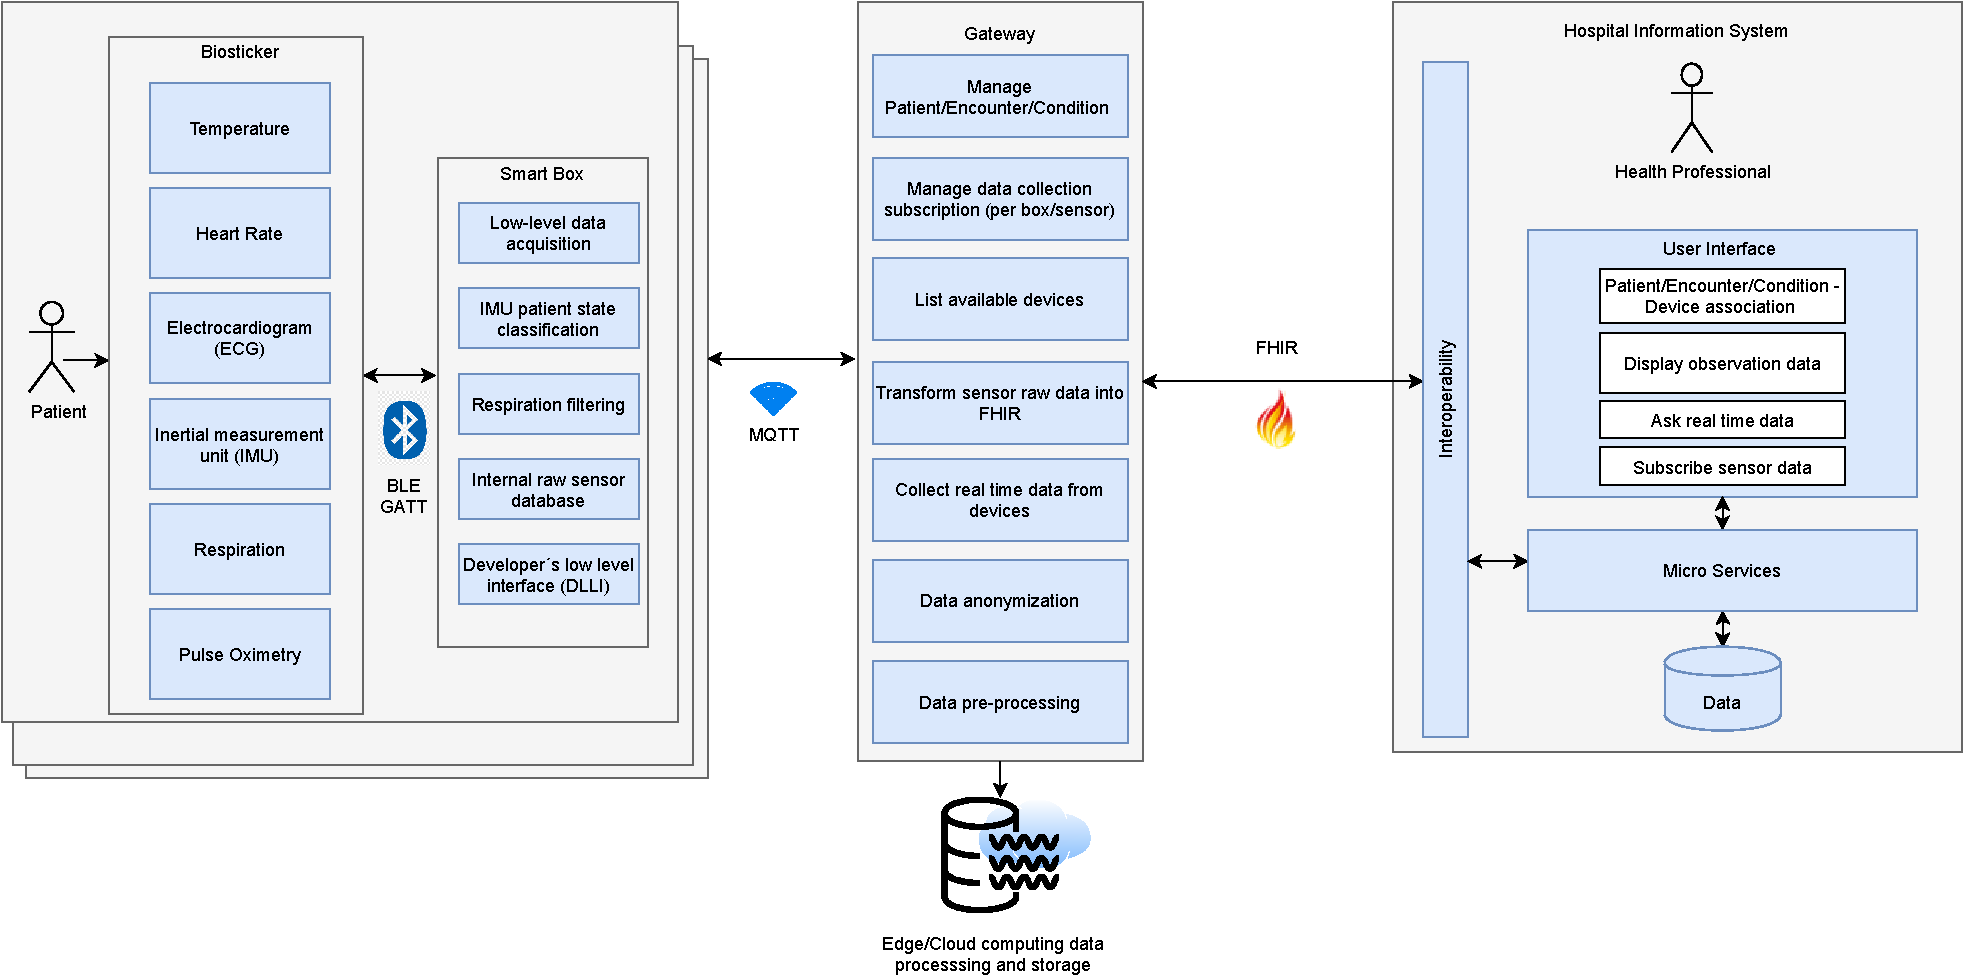
\includegraphics[width=\linewidth]{images/wow-system-architecture.pdf}
    \caption[System architecture of the \acs{WoW} project.]{System architecture of the \acs{WoW} project. In this work, we discuss the implementation of the \textit{Smart Gateway} components, as well as contributions to the \textit{SmartBox} development.}
    \label{fig:wow-architecture}
\end{figure}

For the work developed throughout the dissertation, we propose the following contributions:

\begin{itemize}
    \item Development and deployment of the \textit{SmartBoxes} embedded in hospital beds for data acquisition from \textit{Biostickers} attached to patients’ skin, namely:
    \begin{itemize}
        \item Hardware evaluation of 2 different \acs{IoT} kits (Raspberry Pi and Udoo Bolt).
        \item Evaluation of different \acs{BLE} adapters for data acquisition.
        %\item Selection of hardware components and assembly of SmartBox prototype;
    \end{itemize}
    \item Design and development of data integration pipelines using \acs{MQTT} and management of the multiple SmartBoxes in the Smart Gateway;
    \item Implementation of a \acs{FHIR} \acs{API} layer to integrate the proposed system in the GlobalCare \acs{HIS}.
    \item Evaluation of the performance of the proposed system on hospital trials within the \acs{WoW} project.
    % through controlled lab tests and 
    %\item Evaluate the need for data analysis to extract relevant user profiles/anomalies for long-term biomonitoring data of multiple anonymous users.
\end{itemize}

\section{Summary}
In this chapter, we have discussed the importance of \acs{IoT} systems, how these are composed and how these can bring value to healthcare providers. After analyzing different relevant systems proposed previously in the literature, we have defined a set of criteria to guide the development of our own implementation.

\bigskip

In the next chapter, we begin with the evaluation of the different \acs{IoT} kits for the \textit{Smart Bed} hardware, and afterwards, we evaluate different \acs{BLE} adapters for patient data acquisition to implement secure communications between the \textit{Biostickers} and the \textit{SmartBoxes}. 

% - Hardware evaluation for edge nodes which integrate electronic wireless patches that gather patient's physiological signals;
% - Integrating IoT system in an existing healthcare information system (Glintt GlobalCare software) through an FHIR API layer;
% - Evaluation of the performance of the proposed system through a testbed and a real healthcare scenario;

% In the context of the WoW project, a preliminary study will be performed, by analyzing 24 hours of data from 3 volunteers who are using a specific drug (i.e.! paracetamol) in order to illustrate the effect of the drug intake on various parameters, including temperature, emotions, heart rate, blood oxygen, and respiration.

% Se fizer sentido, na dissertação podes ter um capitulo de "Technological Background", que faz um overview às ferramentas de sotware e ao próprio hardware utilizado no projecto. (to be discussed later)

\bigskip

\chapter{SmartBox Development}
\label{chap:smartbox}

In the proposed architecture, the \textit{SmartBox} plays the role of acquiring the data that is transmitted wirelessly by the \textit{Biostickers}.
Each \textit{SmartBox} is associated to a single patient, it captures the data of each \textit{Biosticker} attached to that patient, and stores it in a local database for redundancy. 
It should also be capable of analyzing and process the data in real time, before propagating it to the higher layers in the system architecture, in order to reduce computation and networking overhead on the Smart Gateway. The \acs{WoW} project also foresees the usage of a classification algorithm in the \textit{SmartBox} to determine the body pose of the patient, as well as filtering the respiration data to account for signal fluctuations caused by sudden movements by the patient.  


\paragraph{} Additionally, for debugging purposes, researchers at the \acs{ISR} developed a simple developer \acs{GUI}, which can be seen on Figure \ref{fig:smartbox-gui}.

\begin{figure}[H]
    \centering
    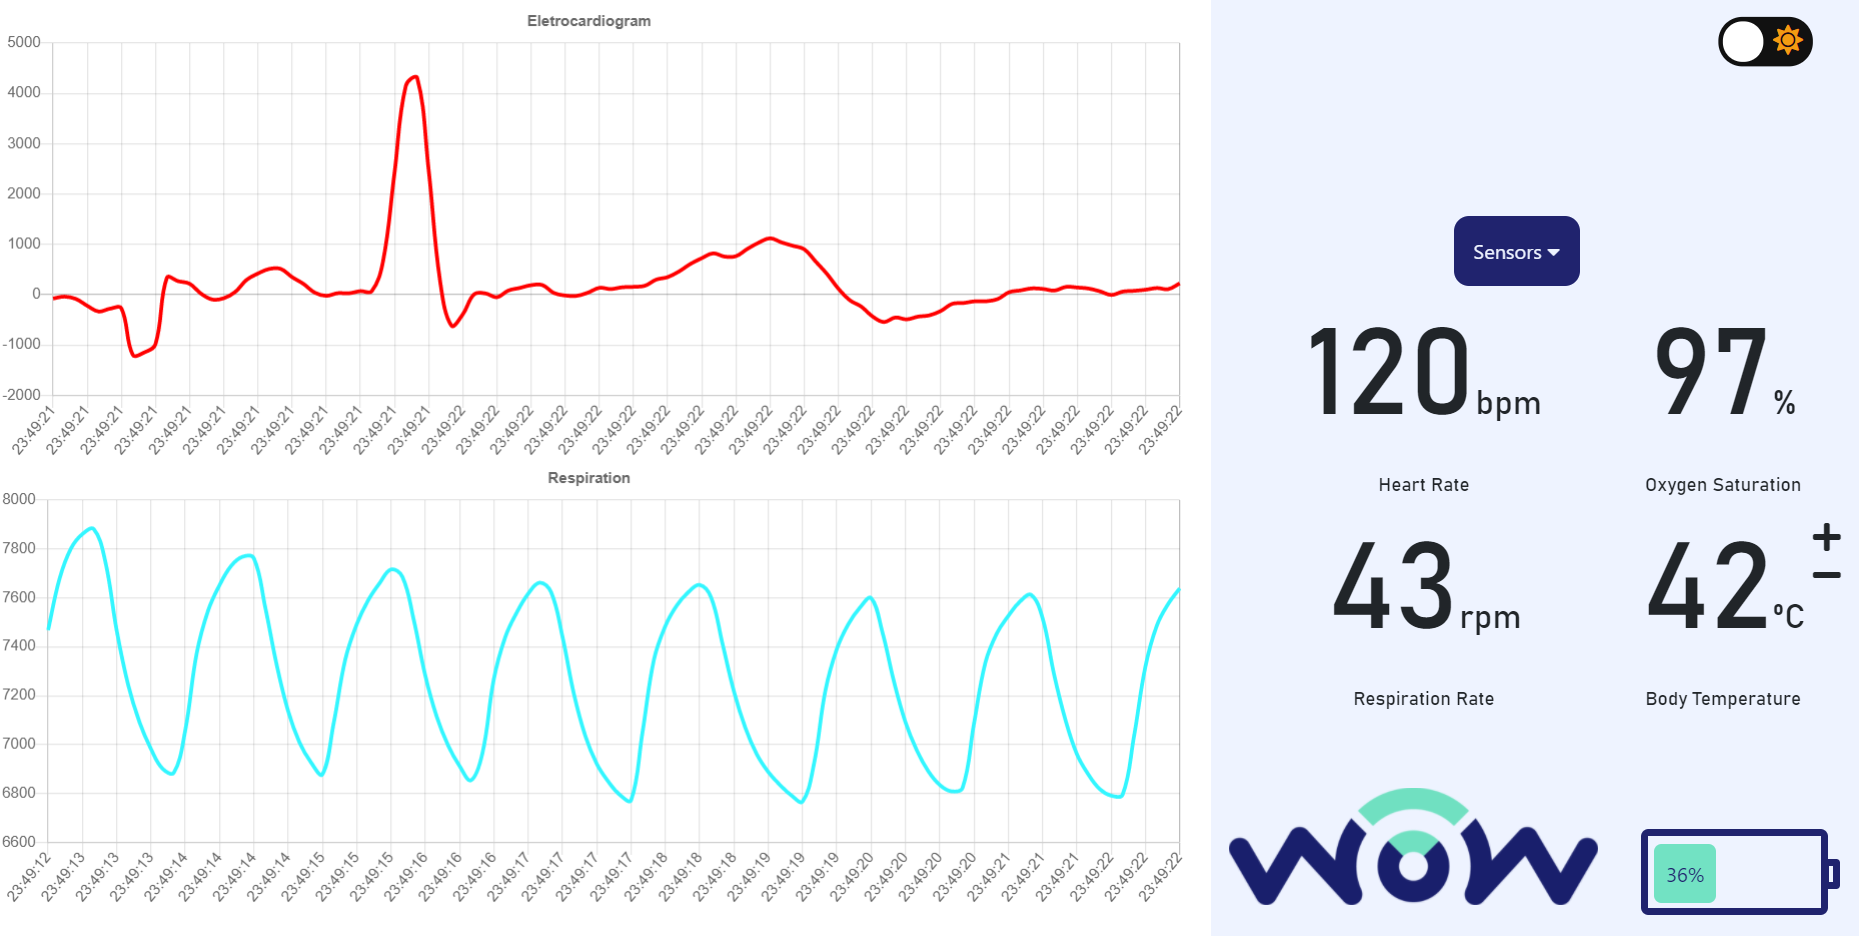
\includegraphics[width=\linewidth]{images/smartbox-gui.png}
    \caption{Illustration of the developer \acf{GUI} for debugging the \textit{SmartBox} acquisition, designed by the \acs{WoW} research team at \acs{ISR}.}
    \label{fig:smartbox-gui}
\end{figure}

\paragraph{} Regarding data acquisition, the \textit{SmartBox} collects 5 distinct biosignals, which can be seen on the developer low level \acs{GUI} on Figure \ref{fig:smartbox-gui}:

\begin{itemize}
    \item \acf{ECG} -- Byte array (20 byte length) with the electrical signal measured, with a frequency of 20Hz.
    \item Respiration Rate -- An unsigned integer (4 bytes) representation of the rate of respiration, with a frequency of 10Hz.
    \item Heart Rate -- An unsigned byte representation of the heart rate in \textit{beats per minute}, every 5s.
    \item Body Temperature -- An IEEE 11073\footnote{\url{https://standards.ieee.org/standard/11073-10207-2017.html}} floating-point number representation of the body temperature, every 60s.
    \item Oxygen Saturation -- A standard floating-point number (4 bytes) representation of the oxygen saturation, with a frequency of 1Hz.
\end{itemize}

\todo[inline]{Todo: Confirm with @Bernardo acquisition rates for each value.}
\todo[inline]{Todo: Ask @Miguel for a picture of the biostickers.}
\section{Deciding on a Hardware Platform}

In the context of this dissertation, two different \acl{SBC}s (\acs{SBC}) were considered for the development of the \textit{SmartBox}: a Raspberry Pi 4 Model B and an UDOO BOLT v3. In the following sections we discuss and compare the characteristics of each platform. 

\subsubsection{Raspberry Pi 4 Model B}

Raspberry Pi denotes a series of \acs{SBC}s which are developed by the Raspberry Pi Foundation, a UK-based charity that aims to educate the general public about the power of computing and digital making, in association with Broadcom. It is one of the most popular hardware platforms used by developers due to its accessible price and community support \cite{jain2021introduction}.
At the time of the writing, the Raspberry Pi 4 Model B (or Raspberry Pi 4B)\footnote{\url{https://www.raspberrypi.com/products/raspberry-pi-4-model-b/}}, which can be seen in Figure \ref{fig:raspberrypi-image}, is the latest revision of the Raspberry Pi series, powered by Broadcom BCM2711 System on a Chip (SoC).

\begin{figure}[H]
    \centering
    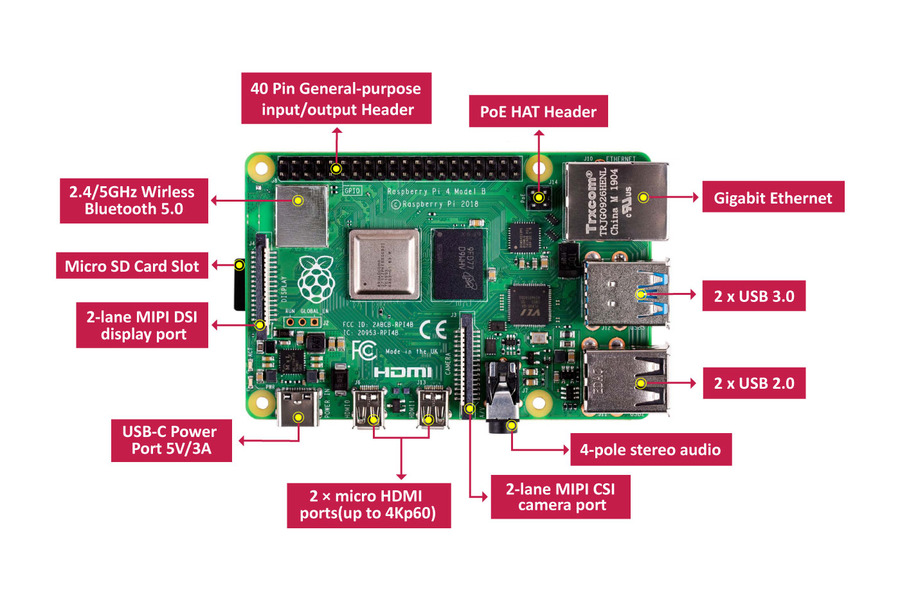
\includegraphics[width=\linewidth]{images/raspberry-4-modele-b-4go.jpg}
    \caption{Raspberry Pi 4B.}
    \label{fig:raspberrypi-image}
\end{figure}

\subsubsection{UDOO BOLT V3}

As stated by the manufacturer\footnote{Product Website: https://www.udoo.org/discover-the-udoo-bolt/}, the ``UDOO BOLT is a quantum leap compared to current maker boards''. It represents a series of high performance \acs{SBC}, equipped with the latest generation of AMD Ryzen Embedded SoC. Additionally, it contains an Arduino Compatible microcontroller (connected via UART), making the UDOO BOLT extremely versatile.
The UDOO Bolt is incredibly well-supported by UDOO but unfortunately, it does not have nearly the same community support of Raspberry Pi.

\paragraph{} The UDOO BOLT V3, which can be seen in Figure \ref{fig:udoobolt-image}, is the entry-level product of the series, but it is still capable of allegedly outperforming full-fledged computers such as the Apple MacBook Pro 13", which just goes to show how powerful these \acs{SBC}s can be.

\todo[inline]{To-do: If time allows it, remake this with better quality.}

\begin{figure}[H]
    \centering
    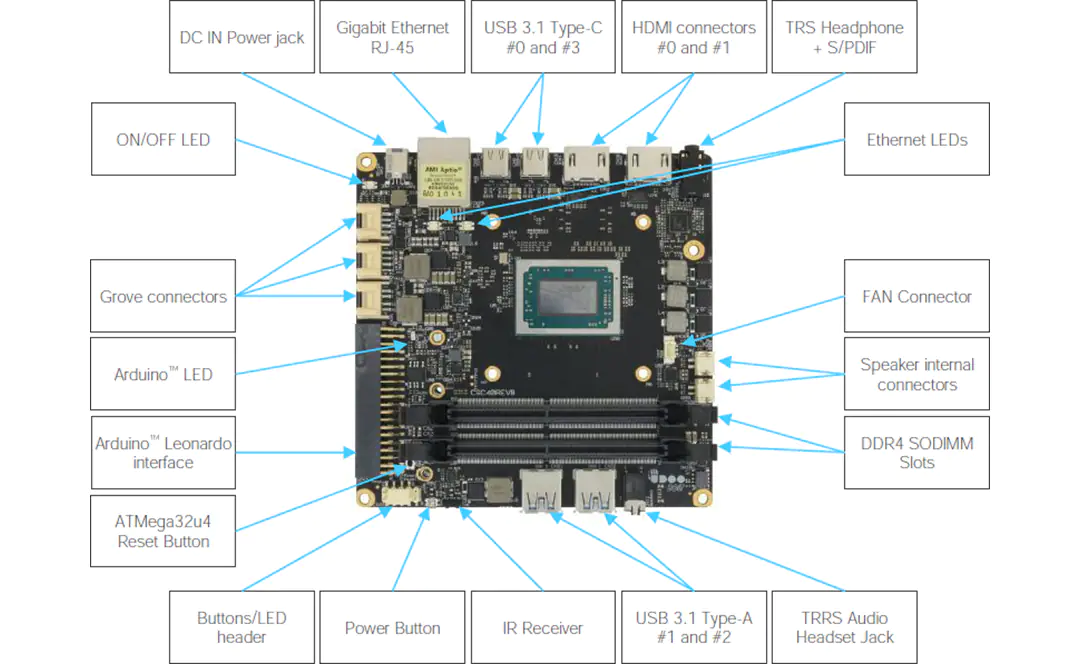
\includegraphics[width=\linewidth]{images/UDOO_BOLT_GEAR_BLT.png}
    \caption{UDOO BOLT V3.}
    \label{fig:udoobolt-image}
\end{figure}

\subsection{Comparing the Hardware Platforms}

In order to decide on which platform to pick for the development of the project, it is crucial to compare the specification of both boards, which can be seen in the Table \ref{tab:comparsion-hardwareplatform}.

\paragraph{} From Table \ref{tab:comparsion-hardwareplatform}, we immediately conclude that the Raspberry Pi is a much more affordable alternative. At over 1/7 of the price, it already has a working WiFi+BT networking module (which is not included in the UDOO BOLT), nearly identical Input/Output (I/O) port capability and a smaller size. UDOO BOLT V3 on the other hand, has a much better SoC, which is expected to delivery a much better overall computing performance.

\renewcommand{\arraystretch}{2.5}
\begin{table}[H]
    \centering
    \begin{tabular}{r|l|l}
        %\textbf{Features} 
        & \textbf{Raspberry Pi 4B}& \textbf{UDOO BOLT V3}  \\ \hline
        \textbf{SoC} &  \makecell{Broadcom BCM2711 \\ (ARMv8 64-bit) \\ 4-core @ 1.5GHz} & \makecell{AMD Ryzen™ Embedded V1202B \\ (AMD64 64-bit) 2-core @ 2.3GHz \\ (up to 3.2GHz turbo)}\\
        \textbf{RAM} & 2, 4 or 8GB LPDDR4 & Up to 32GB DDR4 (Not included) \\ 
        \textbf{Storage} & \makecell{No internal storage, \\ SDXC Card Support} & \makecell{32GB internal eMMC + \\1 × SATA III and \\ 2 × M.2 connectors}\\
        \textbf{Networking} & \makecell{2.4/5.0 GHz WiFi, Gigabit \\ Ethernet, Bluetooth 5.0, BLE} & \makecell{Gigabit Ethernet + M.2 Key E slot \\ for optional WiFi+BT module}\\ 
        \textbf{I/O Ports} & \makecell{ 2 × USB 3.0, 2 × USB 2.0, \\ 2 × (Mini) HDMI} & \makecell{2 × USB 3.0 Type-A, \\ 2 × USB Type-C (w/ Display Port \\ + Power Delivery), 2 × HDMI} \\
        \makecell[r]{\textbf{Other} \\\textbf{Features}} & \makecell{Power over Ethernet \\(PoE)–enabled} & \makecell{Includes ATmega32U4 microcontroller\\ (Arduino Leonardo compatible), \\ RTC Battery} \\   
        \textbf{Dimensions} & 8.5 x 5.6 x 1.7 cm & 12 x 12 x 7 cm \\
        \textbf{Price} & \makecell{75.93 € (\textbf{8GB Model}, \\ including a 32GB SDXC Card\\ and case)} & \makecell{534.48 € (including external power \\ supply and a 16GB RAM module)} \\
    \end{tabular}
    \caption{Specifications of the Raspberry Pi 4B and UDOO BOLT V3.}
    \label{tab:comparsion-hardwareplatform}
\end{table}
\renewcommand{\arraystretch}{1}

\paragraph{} In order to understand how these differences in the hardware specification between the \acs{SBC}s translate to real-world performance, a test suite was developed and conducted to quantify the performance of each \acs{SBC}. The tools developed for each test can be found here\footnote{\url{https://github.com/WoW-Institute-of-Systems-and-Robotics/smartbox\_benchmark\_tests}}. 

\paragraph{}Below, we detail how each test works and discuss how each \acs{SBC} performed. 

\subsubsection{Test 1: Python Benchmark}

Given the data processing requirements for the \textit{SmartBox}, and as Python will be used as the main scripting language for most of the \textit{SmartBox} development, we developed a simple test to estimate computing performance, or more specifically (single-threaded) performance of arithmetic tasks, on each \acs{SBC}. In this test, each \acs{SBC} calculates the \textit{n}-th number in the Fibonacci sequence \cite{pierce1951fibonacci}, and we measure the time taken. This process is repeated 10 times for different numbers, from 10000 to 500000, to determine average run time.

\begin{figure}[H]
    \centering
    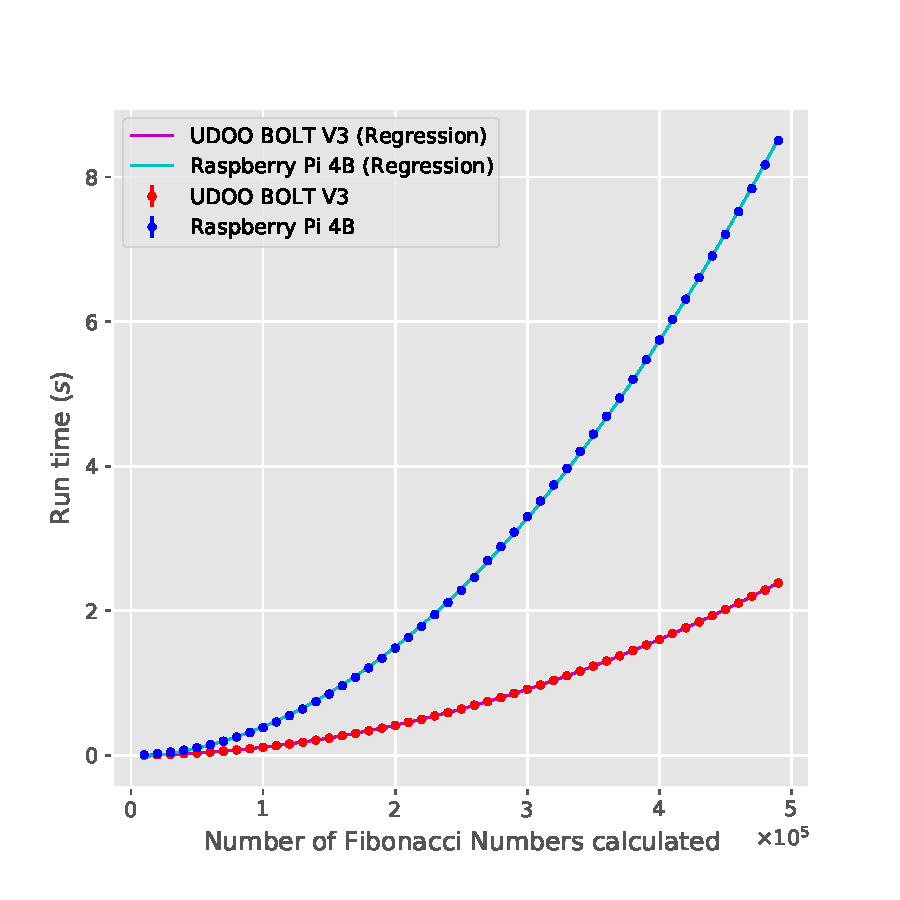
\includegraphics[width=0.8 \linewidth]{images/fibonacci-test.pdf}
    \caption [Custom Python benchmark for the Raspberry Pi 4B and UDOO BOLT V3.]{ Custom Python benchmark for the Raspberry Pi 4B and UDOO BOLT V3. The standard deviation for each run time is inferior to 0.1\% in each test, and therefore it is not displayed in the figure.}
    \label{fig:fibonacci-tests}
\end{figure}

From Figure \ref{fig:fibonacci-tests}, we can observe that the time taken for computing each number increases exponentially for each platform. By analyzing the data, we can see that the UDOO BOLT V3 outperforms Raspberry Pi 4B on average by a factor of 2.5 $\pm$ 0.2.

\subsubsection{Test 2: Phoronix Test Suite}

The Phoronix Test Suite\footnote{Phoronix Test Suite - Linux Testing \& Benchmarking Platform, Automated Testing, Open-Source Benchmarking: \url{https://www.phoronix-test-suite.com/}} is an open-source benchmarking platform used for comparing the performance of different systems. The framework provides compilations of tests for a variety of tools and is also fully customizable and expandable, allowing users to develop and automate their own tests in a clean, reproducible and easy-to-use fashion. The test profiles work by measuring some property of the benchmark, (\textit{e.g.} the run time for calculating the first 100 Fibonacci numbers) and use it to provide an estimate of the performance of the \acs{SBC}, which can be easily used for comparison between different systems. 

\paragraph{} For the purposes of evaluating the computing performance of each \acs{SBC}, we chose the following standard test profiles provided by Phoronix\footnote{OpenBenchmarking.org - Cross-Platform, Open-Source Automated Benchmarking Platform: \url{https://openbenchmarking.org/}}, which are a compilation of the most popular Python and CPU benchmarks used \footnote{The benchmark results obtained were published in the \textit{OpenBenchmarking.org} website, and can be found by visiting the following webpage: \url{https://openbenchmarking.org/result/2110255-JNCF-211025851}.}:

\begin{itemize}
    \item BYTE Unix Benchmark (``BYTE''), single-threaded CPU benchmark -- Runs BYTE UNIX benchmark suite (more particularly, the Dhrystone 2 synthetic benchmark) to measure the amount of instructions per second (IPS). 
    \item 7-Zip Compression (``7-Zip''), multithreaded CPU benchmark -- Runs the benchmark feature integrated in 7-Zip to measure the amount of millions instructions per second (MIPS). The benchmark consists of a LZMA data compression and decompression test run, using all available threads in the system (meaning it will scale highly with the amount of threads in the system). 
    \item PyBench Benchmark (``PyBench''), single-threaded Python \& CPU benchmark -- Executes different function such as built-in function calls and nested for-loops and measures its runtime.
    \item PyPerformance \textit{chaos} Benchmark (``chaos''), single-threaded Python \& CPU benchmark -- Create chaos game-like fractals \cite{Jeffrey1992} and measures its run-time. 
    \item PyPerformance \textit{float} Benchmark (``float''), single-threaded Python \& CPU benchmark -- Create 100,000 random floating-point numbers and calculate the co-sine, sine and square root of each one and measures its run-time.
    \item PyPerformance \textit{nbody} Benchmark (``nbody''), single-threaded Python \& CPU benchmark -- Runs an \textit{n-body} problem simulation \cite{Playne2009} and measures its run-time.
    \item PyPerformance \textit{json\_loads} Benchmark (``json''), single-threaded Python \& CPU benchmark -- Evaluates \acf{JSON}\footnote{The JavaScript Object Notation (JSON) Data Interchange Format: \url{https://www.rfc-editor.org/rfc/rfc8259.html}} parsing and serialization, a widely used open stardard data format, by dumping and loading thousands of objects and measures its runtime.
    \item PyPerformance \textit{crypto\_pyaes} Benchmark (``crypto''), single-threaded Python \& CPU benchmark -- Runs the AES block-cipher Python implementation and measures its run-time.
    \item PyPerformance \textit{regex\_compile} Benchmark (``regex''), single-threaded Python \& CPU benchmark -- Compiles different \textit{regular expressions} or \textit{regexes} in Python and measures its run-time.
    \item PyPerformance \textit{python\_startup} Benchmark (``startup''), single-threaded Python \& general system performance benchmark -- Measures Python's startup time.
    \item PyPerformance \textit{django\_template} Benchmark (``django''), single-threaded Python benchmark -- Builds a 150x150-cell HTML table and measures its run-time.
\end{itemize}

\begin{figure}[H]
    \centering
    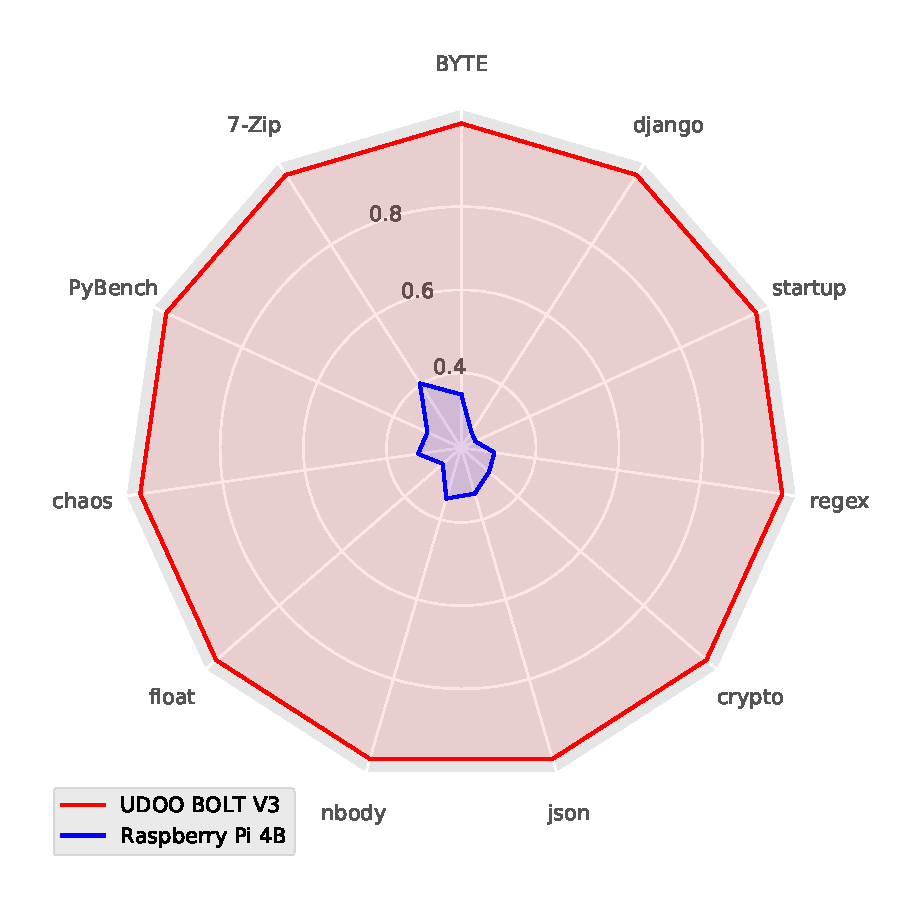
\includegraphics[width=0.8 \linewidth]{images/phoronix-benchmarks.pdf}
    \caption [Phoronix benchmarks for the UDOO BOLT V3 and Raspberry Pi 4B.]{ Phoronix benchmarks for the UDOO BOLT V3 and Raspberry Pi 4B. The performance values for each test are normalized to UDOO BOLT V3 performance.}
    \label{fig:phronix-benchmarks}
\end{figure}

\paragraph{} From Figure \ref{fig:phronix-benchmarks}, we can observe that UDOO BOLT V3 performs much better than Raspberry Pi 4B in every benchmark, as expected. We also notice some disparity in the relative performance throughout the benchmarks, in particular, the 7-Zip benchmark. This is likely due to the fact that 7-Zip benchmark is a multithreaded test, and as Raspberry Pi 4B has more threads than UDOO BOLT V3, it manages to close the performance gap (albeit only slightly). By analyzing the data, we find that UDOO BOLT V3 outperforms Raspberry Pi 4B on average by a factor of 2.21 $\pm$ 0.4.

\subsubsection{Test 3: \acs{MQTT} Benchmark}

As the \textit{SmartBox} is intended to communicate with the Smart Gateway through \acs{MQTT} messages, we also evaluate how each system handles the load associated with an \acs{MQTT} client. For this test, each \acs{SBC} ran a simple \acs{MQTT} client, which subscribes to a single topic and publishes a message to another topic at a given transmission rate, with a payload containing the string ``hello world'', through an \acs{MQTT} broker in the local network.

\todo[inline]{To-do: Repeat tests with higher rates if time allows it.}
\begin{figure}[H]
    \centering
    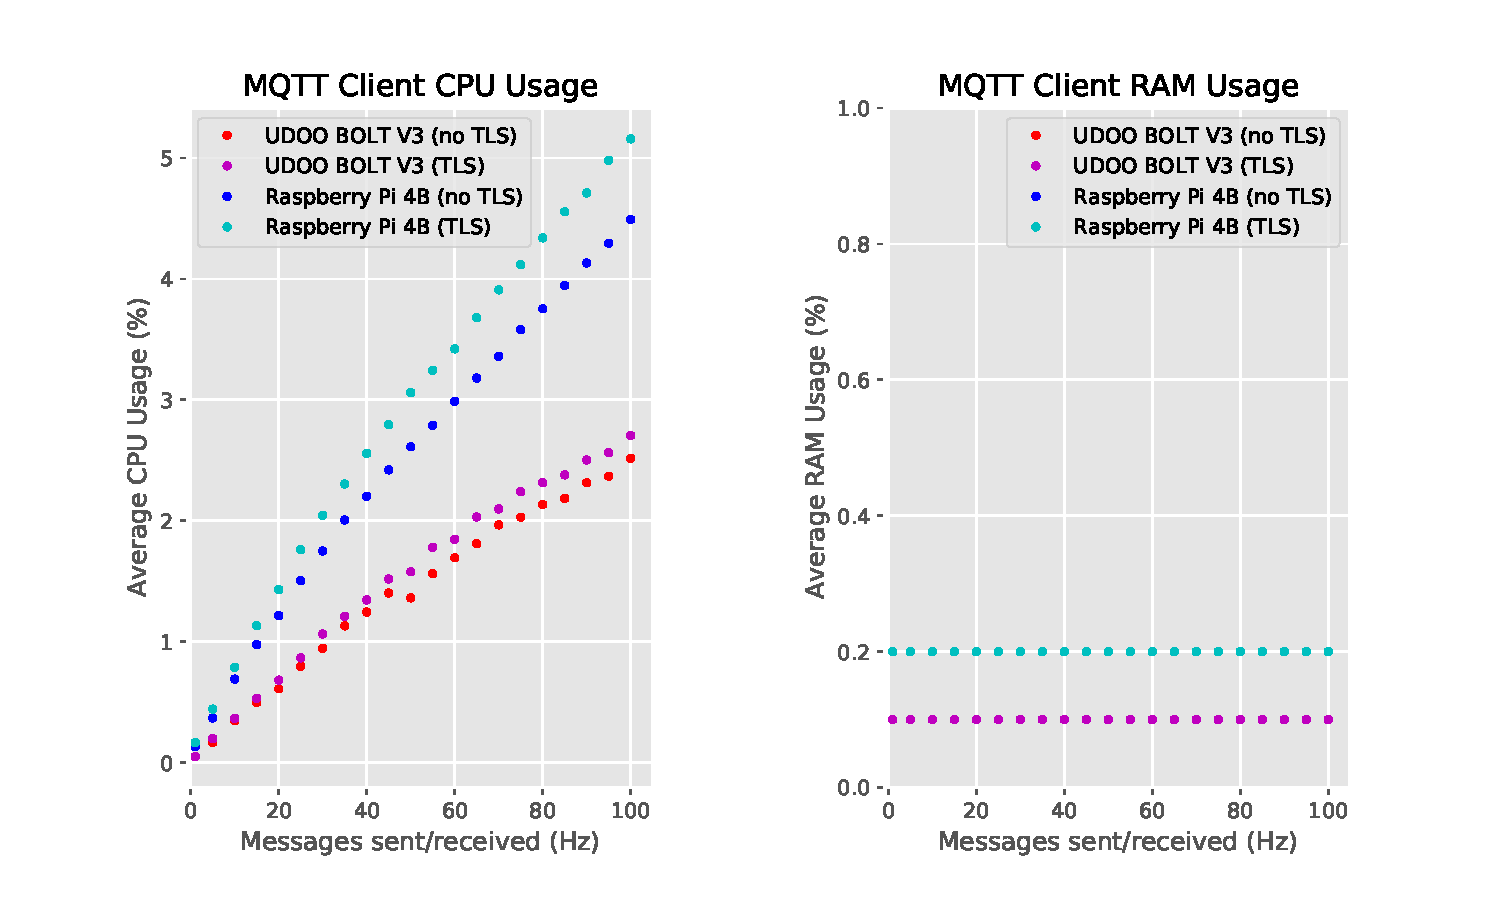
\includegraphics[width=\linewidth]{images/mqtt_test_results.pdf}
    \caption[\acs{MQTT} benchmark for Raspberry Pi 4B and UDOO BOLT V3.]{\acs{MQTT} benchmark for Raspberry Pi 4B and UDOO BOLT V3. As the transmission frequency increases, we observe that the Raspberry Pi consumes more resources than the UDOO BOLT V3, nonetheless, these are very negligible performance differences, with an impact of < 0.5\% resource usage.}
    \label{fig:mqtt-tests}
\end{figure}

The \acs{MQTT} client is a very lightweight process, and as seen in Figure \ref{fig:mqtt-tests}, it is capable of running on both platforms with trivial performance impact.

\subsection{Final Decision on SmartBox hardware}

Based on the results of our tests we conclude that UDOO BOLT V3 heavily outperforms the Raspberry Pi 4B in CPU benchmarks, but shows a negligible difference in memory usage. Nonetheless, we find that these performance gains do not meaningfully impact the \textit{SmartBox} functionality, for example, in the \acs{MQTT} communication. We can also extend this to other features, such as the developer \acs{GUI} or the Python acquisition script, which should have a similar resource load to the \acs{MQTT} client in the previous \acs{MQTT} benchmark.

\paragraph{} Additionally, the Raspberry Pi 4B comes out of the box with an included WiFi+\acs{BLE} combo networking card, 8GB of RAM (as we chose the 8GB model), and a much smaller form factor -- which is very useful for embedding the \textit{SmartBox} in the \textit{SmartBeds}. And this is at 1/7 the cost of UDOO BOLT V3, making this much more affordable to scale and replicate the system with many \textit{SmartBoxes}.

\paragraph{} Due to all of the aforementioned reasons, we have decided to move forward with the Raspberry Pi 4B for the \textit{SmartBox} development in the scope of the \acs{WoW} project.

\section{Communication with the Biostickers}

As previously mentioned, the communication between the \textit{Biostickers} and the \textit{SmartBox} makes use of the \acs{BLE} protocol. One of the advantages of using the Raspberry Pi 4B, as discussed in the previous section, is the fact that it already includes all networking functionality needed for the project. 

% explicar pra que serve e q sinal adquire

\paragraph{} However, the communication with the \textit{Biostickers} is very critical and demanding. During the development of the project, the research team has decided to use a \textit{Biosticker} coupled with a commercially available Pulse Oximeter -- used to measure oxygen saturation at the finger tip --  in order to capture all required biosignals. This means that the \acs{BLE} acquisition system must be capable of handling both communications simultaneously. Having this in mind, we need to understand if the included \acs{BLE} adapter of the Raspberry Pi board is sufficient for the task, or if we need to consider a different acquisition hardware.

\paragraph{} In order to understand how data transmission works between \acs{BLE} devices, some technical background regarding the data transmission in protocol is presented.

\subsection{Technical Background} 
 % Ver https://www.scirp.org/journal/paperinformation.aspx?paperid=103686

% \todo[inline]{To-do: Intro to Link Layer, LE 1M e 2M, packet format, mention GATT and overview data transmission...}

The \acs{BLE} protocol stack is organized into three major components, as shown in Figure \ref{fig:ble-protocol-stack}: the Application Layer, the Host Layer and Controller Layer. 

\begin{figure}[H]
    \centering
    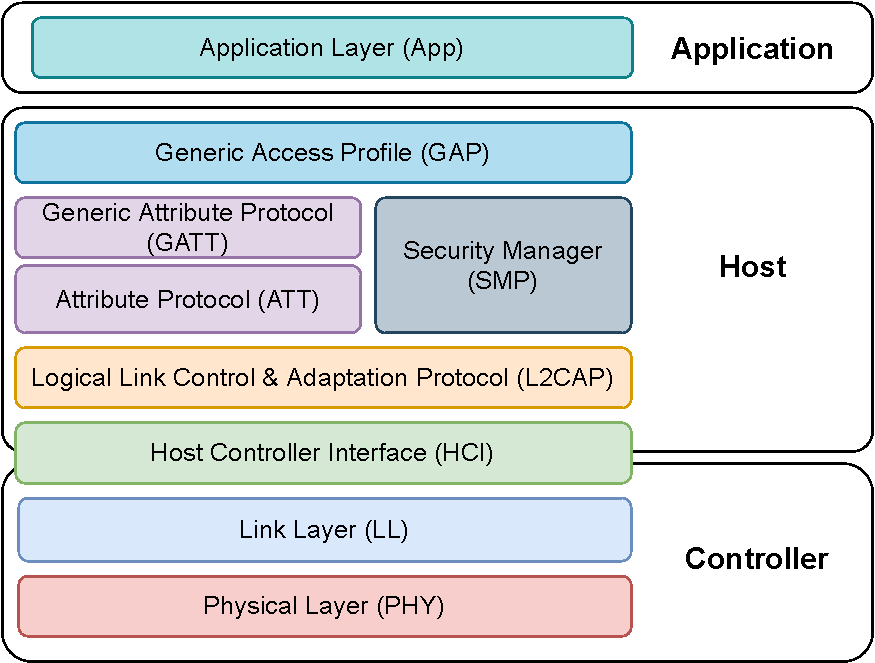
\includegraphics[width=0.6\linewidth]{images/ble protocol stack.pdf}
    \caption[Diagram of the different components of the \acs{BLE} protocol stack.]{Diagram of the different components of the \acs{BLE} protocol stack. Adapted from \cite{Specification1999, Farej2020}}
    \label{fig:ble-protocol-stack}
\end{figure}

At the Controller layer, we have the \acf{PHY} and \acf{LL} components. 

The \acf{PHY} is the bottom layer of the \acs{BLE} stack, and is responsible for the transmission and reception of information over radio waves on the Industrial Scientific Medical (ISM) 2.4GHz band. According to the latest revision of the specification \cite{Specification1999}, \acs{BLE} supports 3 distinct physical layers: LE 1M, LE 2M and LE Coded. The first is the default \acs{PHY}, with a data rate of 1 Mbps, which existed in previous versions of Bluetooth, the latter 2 were introduced in Bluetooth 5. LE 2M is an upgrade of the previous \acs{PHY}, doubling the data rate to 2 Mbps, and LE Coded has a much larger range (up to 4x), at cost of a lower data rate (500 kbps or 125 kbps). 

The \acf{LL} layer interfaces directly with the \acs{PHY}, and manages the link state of the radio. It also provides the mechanism for the higher layers to interact with the radio transceiver. 

\paragraph{} Afterwards, we have the Host Layer, containing the higher level components of the protocol stack that interact with the application level layers. The \acs{L2CAP} is responsible for managing the data between the \acs{LL} and the higher layers in the protocol stack. It abstracts the communication details from the higher layers, handling seamlessly the fragmentation of the data into multiple \acs{LL} data packets for transmission and reassembly of \acs{LL} data packets for higher layer protocols such as \acf{ATT}.

\acs{ATT} is the protocol used to expose the application data to other \acs{BLE} devices through data structured called ``Attributes'', which are smallest addressable units of data used by \acs{ATT}. From the application point of view, data is exchanged using \acf{GATT}, which can be viewed as a ``meta-layed'' on top of \acs{ATT}. Regarding \acs{GATT} there are 3 main constructs to consider:

\begin{itemize}
    \item \acs{GATT} Characteristic -- The lowest level concept in \acs{GATT} transactions is the Characteristic, which encapsulates a single data point, \textit{e.g.} a temperature measurement, a accelerometer reading, etc. It also defines the different types of interactions, such as reading, writing, subscribing for notifications, etc.
    \item \acs{GATT} Service -- A collection of \acs{GATT} characteristics.
    \item \acs{GATT} Profile -- A collection of Services, usually predefined by Bluetooth SIG, but can also be a custom profile.
\end{itemize}

The \acf{SMP} handles the security in the data transmissions, containing the security algorithms used to encrypt and decrypt the communication.

\paragraph{} The Application Layer contains the user application, which interfaces with the Bluetooth protocol stack.

\paragraph{} The data packet format for \acs{BLE} transmissions is displayed in Figure \ref{fig:ble-ll-packet-format}, showing how the data is encapsulated for the transmission.

\begin{figure}[H]
    \centering
    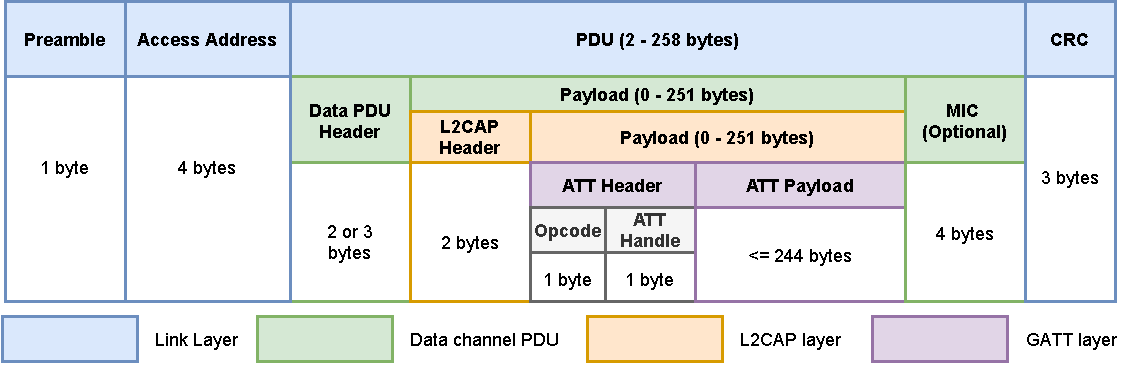
\includegraphics[width=\linewidth]{images/bluetooth data packet format.pdf}
    \caption[Diagram of the \acs{BLE} data packet format for uncoded \acs{PHY}s (LE 1M and LE 2M).]{\acs{BLE} data packet format for uncoded \acs{PHY}s (LE 1M and LE 2M). Adapted from \cite{Specification1999, Farej2020}. The Message Integrity Check (MIC) and Cyclic Redundancy Check (CRC), which are not discussed above, are used for validating the integrity of the data packet.}
    \label{fig:ble-ll-packet-format}
\end{figure}


\paragraph{} Before we discuss \acs{BLE} data transmissions, it is important to expose certain terminology which is used in the area:

\begin{itemize}
    \item Central device (or master): Device that initiates commands and requests.
    \item Peripheral device (or slave): Device that receives commands and requests, and returns responses.
    \item Connection Event: Moment of the connection where the devices engage in radio transmissions.
\end{itemize}

\paragraph{} Figure \ref{fig:ble-message-sequence-chart} shows a single communication event during a \acs{BLE} communication between two devices, A and B. When the device A wants to communicate to the device B, the data must be first fragmented into different \acs{LL} data packets on the \acs{L2CAP} layer, which for this simple example is not considered. The data is transmitted to device B through the \acs{LL} layer, and the data is then reassembled on device B. One thing to consider is that, although there are not rules enforcing the Connection Event to have just transmit one data packet, some \acs{BLE} protocol stack implementation may not support sending more than one packet per Connection Event. 


\begin{figure}[H]
    \centering
    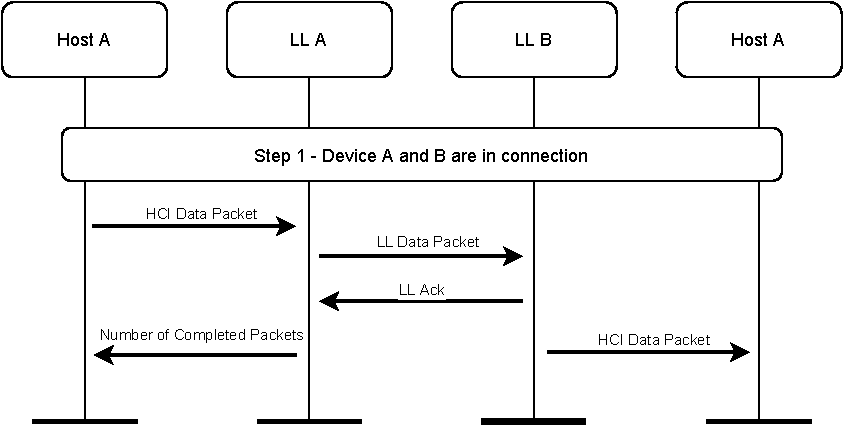
\includegraphics[width=\linewidth]{images/ble-sending-data.pdf}
    \caption[Message sequence chart between two \acs{BLE} devices sending data and replying to the request.]{Message sequence chart between two \acs{BLE} devices sending data and replying to the request. Source: \cite{Specification1999}}
    \label{fig:ble-message-sequence-chart}
\end{figure}

\paragraph{} There are multiple parameters which guide how \acs{BLE} data connections are performed, which are the following: 
\begin{itemize}
    \item Slave Latency: Number of consecutive connection events the slave device is not required to listen for the master. It allows a slave to use a reduced number of connection events, thus minimizing power consumption.
    \item Connection Interval: Time between two consecutive connection events.
    \item Supervisor Timeout: Maximum time between two received data \acs{PDU}s before the connection is considered lost.
    \item \acf{MTU} for the \acs{ATT} protocol: Length of the \acs{PDU} for the \acs{ATT} protocol, which includes the \acs{ATT} header as well as the payload containing the data to be transmitted.
\end{itemize}

\subsubsection{\acs{BLE} protocol stack on Linux} 

In the \acs{WoW} project, the data acquisition is developed using the official Linux implementation of \acs{BLE} protocol stack\footnote{\textit{BlueZ}: \url{http://www.bluez.org/profiles/}} -- \textit{BlueZ} -- in order to promote interoperability; since these drivers are developed and used by the community, allowing us to use multiple \acs{BLE} adapters, and even different \acs{SBC}s, using the same codebase without being tied down to proprietary code. 

% \paragraph{} Currently, \textit{BlueZ} only officially supports up to the Bluetooth 4.2 specification, which is, at the time of writing, is still the predominantly used version \cite{Faria2020}. Nonetheless, Bluetooth specifications are generally backwards compatible with older versions.

% \todo[inline]{Nota para @David Portugal: Isto é o que está indicado no website, mas existem funcionalidades de Bluetooth 5.X que estão implementadas (mas não especificam o escopo que está implementado). Indico alguma coisa sobre isso? Removo este parágrafo? Ou deixo tudo como está? }


\subsection{Choosing a \acs{BLE} adapter} 

\paragraph{} As mentioned previously, one of the objectives of this dissertation work is to analyze if the internal \acs{BLE} adapter provided by the Raspberry Pi 4B is sufficient for the \acs{WoW} project. To achieve this, we decided to compare this adapter with a commercially available that met the requirements for the project. The requirements for the adapter are the following:

\begin{itemize}
    \item The adapter must support, at least, the Bluetooth 5.0 core specification.
    \item The adapter must natively support Ubuntu 20.04, as well as the \textit{BlueZ} \acs{BLE} protocol stack. 
    %\item The adapter should support the LE 2M physical layer for better throughput.
\end{itemize}

\paragraph{} After researching the available market, we chose the Asus USB-BT500 USB adapter\footnote{Asus USB-BT500 Bluetooth 5.0 USB Adapter: \url{https://www.asus.com/Networking-IoT-Servers/Adapters/All-series/USB-BT500/}} due to its affordability and availability, making it an adequate fit for the project's needs.

\paragraph{} In the next section, we perform multiple tests to evaluate the performance of Asus USB-BT500 and the internal \acs{BLE} adapter in the Raspberry Pi 4B.

\subsection{Testing \acs{BLE} Communication} 

To ensure an \acs{BLE} adapter is capable of handling the communication on the \textit{SmartBox} side for the \acs{WoW} project, we created two different tests to evaluate their performance at different distances: a test to evaluate the roundtrip time for a single message (for different sizes), and a test to evaluate the maximum bandwidth achieveable using a packet loss analysis for multiple frequencies.

\paragraph{} For these tests, we need to ensure the conditions are very similar to those when acquiring data from the \textit{Biostickers}. To this end, we use the same microcontroller -- nRF52832 \acs{SoC} -- which is used in the \textit{Biostickers}, with our own custom firmware for the tests. Therefore, the device which is used for ``simulating'' the \acs{BLE} device for the tests is the nRF52-DK developer kit\footnote{\url{https://www.nordicsemi.com/Products/Development-hardware/nrf52-dk}}. The firmware for the microcontroller is built using the latest version of MbedOS\footnote{\url{https://os.mbed.com/mbed-os/}} and can be found here\footnote{\url{https://github.com/WoW-Institute-of-Systems-and-Robotics/ble-test-firmwares/}}.

\subsubsection{Test Conditions}

In order to ensure replicability and reliability of the test results, we use the same connection parameters for all tests, which are the following:

\begin{table}[H]
    \centering
    \begin{tabular}{|l|l|}
    \hline
    \textbf{Connection Interval} & 7.5ms \\ \hline
    \textbf{Slave Latency}       & 0     \\ \hline
    \textbf{Supervisor Timeout}  & 500ms \\ \hline
    \textbf{\acs{ATT} \acs{MTU} Length}      & 23 bytes   \\ \hline
    \end{tabular}
    \caption{\acs{BLE} connection parameters used for the ASUS USB-BT500 adapter.}
    \label{tab:ble-connection-values-hci1}
\end{table}

\begin{table}[H]
    \centering
    \begin{tabular}{|l|l|}
    \hline
    \textbf{Connection Interval} & 7.5ms \\ \hline
    \textbf{Slave Latency}       & 0     \\ \hline
    \textbf{Supervisor Timeout}  & 500ms \\ \hline
    \textbf{\acs{ATT} \acs{MTU} Length}      & 251 bytes   \\ \hline
    \end{tabular}
    \caption{\acs{BLE} connection parameters used for internal Raspberry Pi 4B adapter.}
    \label{tab:ble-connection-values-hci0}
\end{table}

Additionally, these tests were conducted indoors, with the devices (the \acs{BLE} adapter and the microcontroller) in clear view of each other.

\subsubsection{Test 1: Roundtrip Time Measurement}

In this first test, we measure the roundtrip time of a single \acs{ATT} data packet on a \acs{BLE} connection for different payload sizes. For this test, the nRF52-DK board exposed two \acs{GATT} characteristics: one to be updated by the \textit{SmartBox} (characteristic ``A''), and one to which the \textit{SmartBox} subscribed (characteristic ``B''). When the \textit{SmartBox} writes on characteristic ``A'', the nRF52-DK changed the value of the characteristic ``B'', immediately sending a notification to the \textit{SmartBox}. The roundtrip time for our purposes is then the time taken to recieve the notification on characteristic ``B'' after updating the value of characteristic ``A''. Below, are the roundtrip time graphs for different payload sizes obtained for each adapter at different distances. Each test was run 5 times to ensure the results are consistent.

\begin{figure}[H]
    \centering
    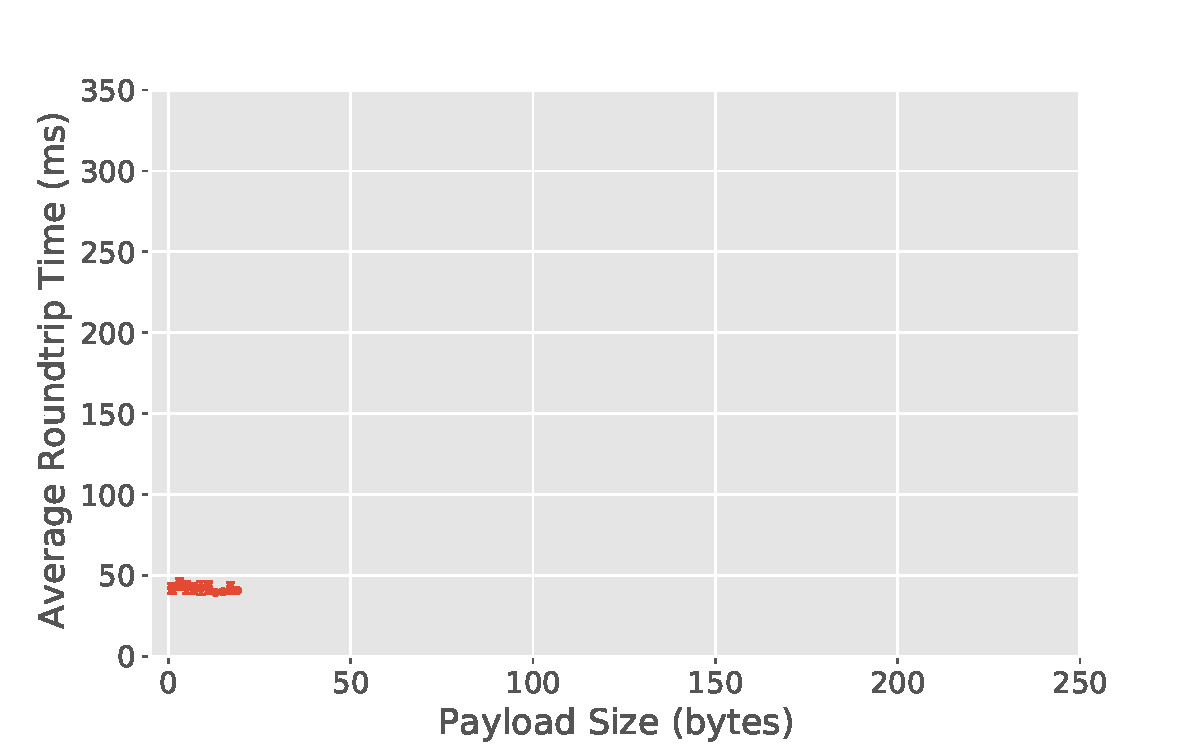
\includegraphics[width=0.75\linewidth]{images/ble-roundtrip-hci1-0cm.pdf}
    \label{fig:ble-roundtrip-hci1-0m}
    \caption[Average \acs{BLE} connection roundtrip time obtained using Raspberry Pi 4B's internal \acs{BLE} adapter at a distance of 0m.]{Average \acs{BLE} connection roundtrip time obtained using Raspberry Pi 4B's internal \acs{BLE} adapter at a distance of $0\text{m} \pm 0.2$.}
\end{figure}

\begin{figure}[H]
    \centering
    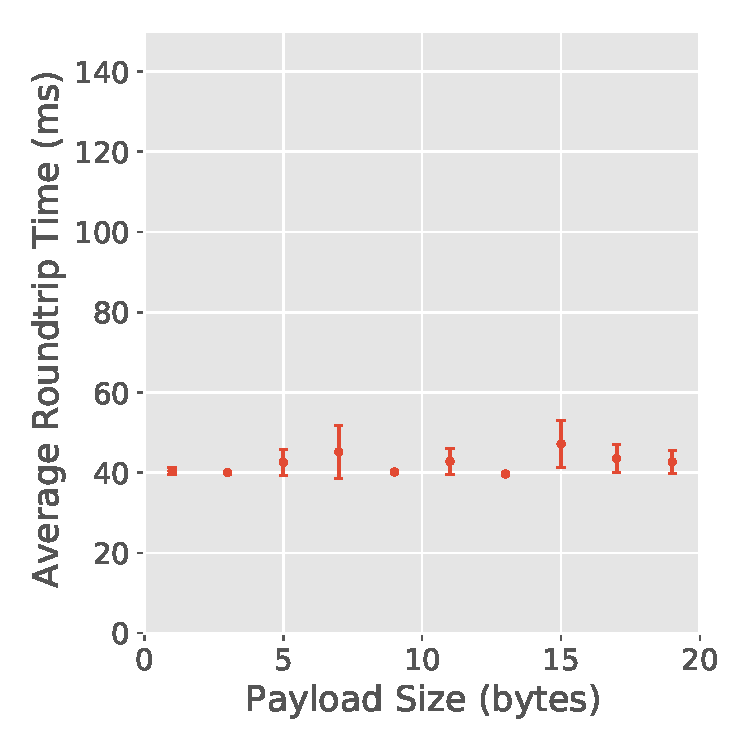
\includegraphics[width=0.75\linewidth]{images/ble-roundtrip-hci1-300cm.pdf}
    \label{fig:ble-roundtrip-hci1-3m}
    \caption[Average \acs{BLE} connection roundtrip time obtained using Raspberry Pi 4B's internal \acs{BLE} adapter at a distance of 3m.]{Average \acs{BLE} connection roundtrip time obtained using Raspberry Pi 4B's internal \acs{BLE} adapter at a distance of $3\text{m} \pm 0.2$.}
\end{figure}

\begin{figure}[H]
    \centering
    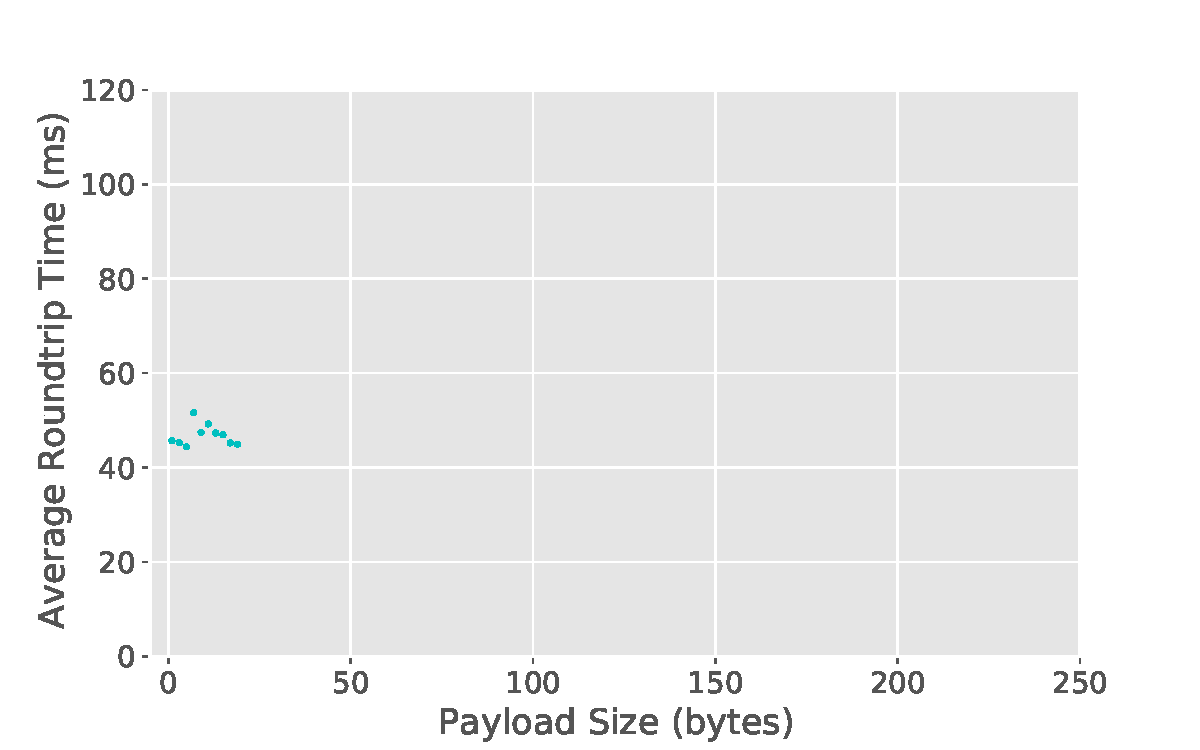
\includegraphics[width=0.75\linewidth]{images/ble-roundtrip-hci1-600cm.pdf}
    \label{fig:ble-roundtrip-hci1-6m}
    \caption[Average \acs{BLE} connection roundtrip time obtained using Raspberry Pi 4B's internal \acs{BLE} adapter at a distance of 6m.]{Average \acs{BLE} connection roundtrip time obtained using Raspberry Pi 4B's internal \acs{BLE} adapter at a distance of $6\text{m} \pm 0.2$.}
\end{figure}

\begin{figure}[H]
    \centering
    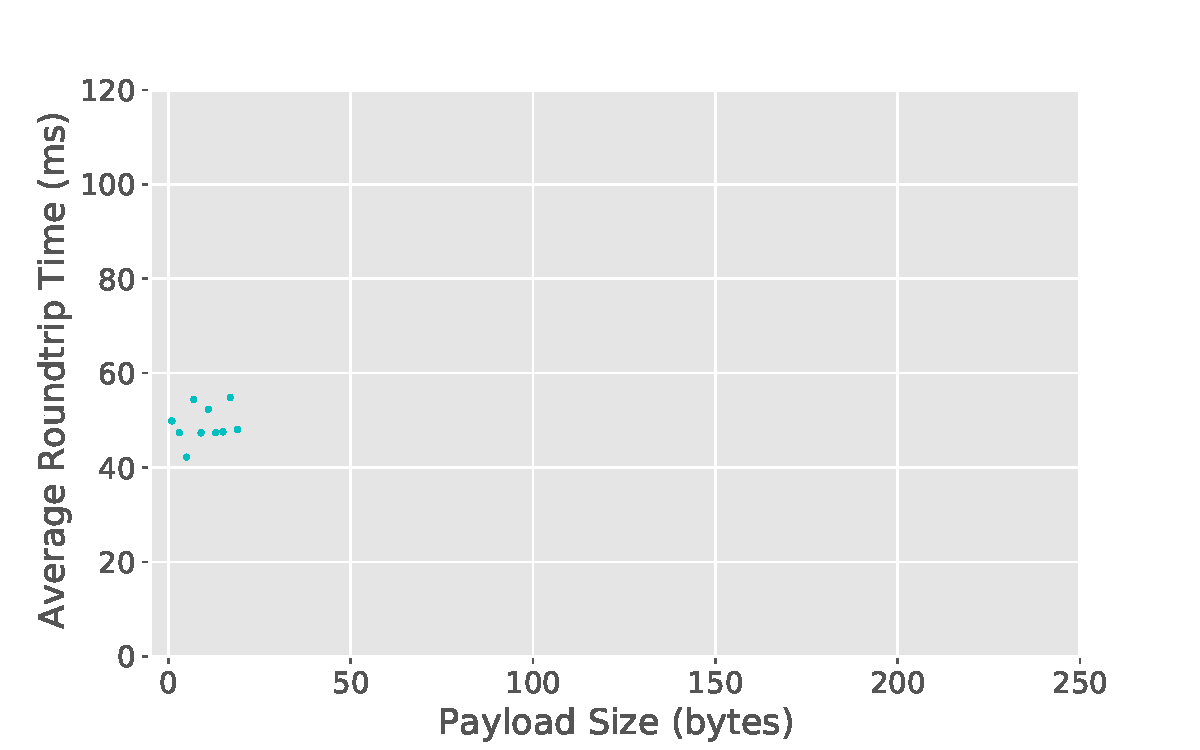
\includegraphics[width=0.75\linewidth]{images/ble-roundtrip-hci1-900cm.pdf}
    \label{fig:ble-roundtrip-hci1-9m}
    \caption[Average \acs{BLE} connection roundtrip time obtained using Raspberry Pi 4B's internal \acs{BLE} adapter at a distance of 9m.]{Average \acs{BLE} connection roundtrip time obtained using Raspberry Pi 4B's internal \acs{BLE} adapter at a distance of $9\text{m} \pm 0.2$.}
\end{figure}

\begin{figure}[H]
    \centering
    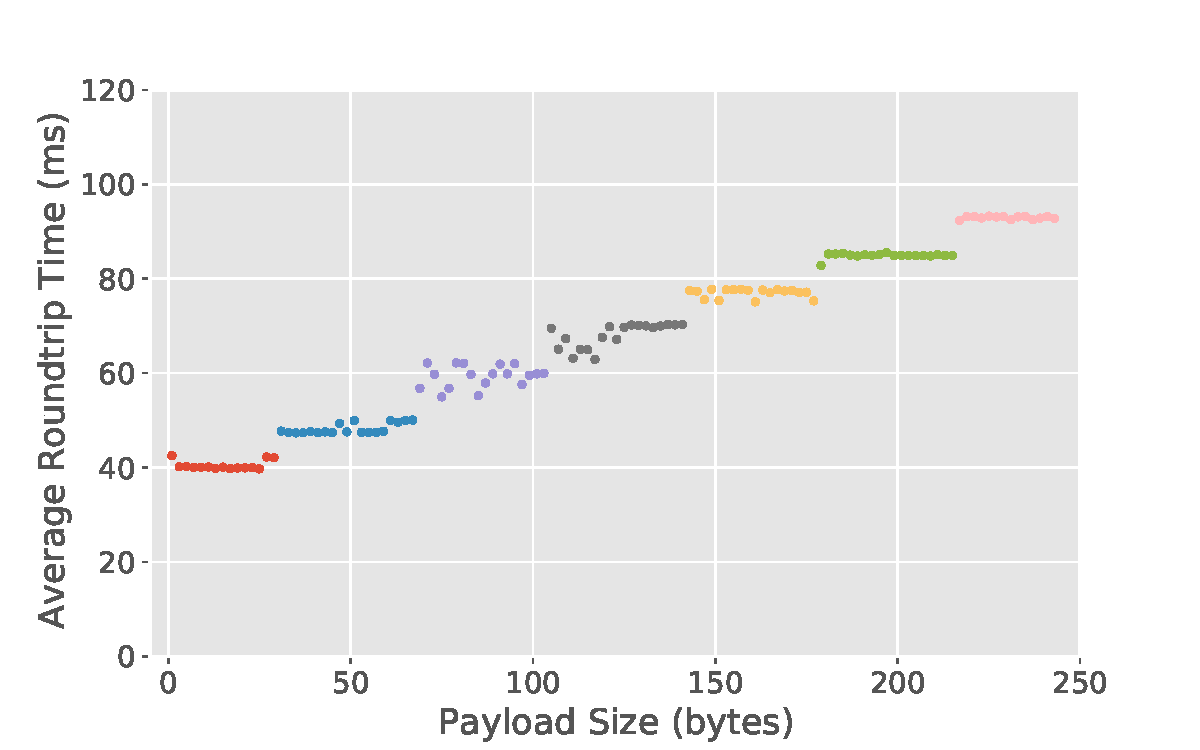
\includegraphics[width=0.75\linewidth]{images/ble-roundtrip-hci0-0cm.pdf}
    \label{fig:ble-roundtrip-hci0-0m}
    \caption[Average \acs{BLE} connection roundtrip time obtained using the Asus USB-BT500 adapter at a distance of 0m.]{Average \acs{BLE} connection roundtrip time obtained using the Asus USB-BT500 adapter at a distance of $0\text{m} \pm 0.2$.}
\end{figure}

\begin{figure}[H]
    \centering
    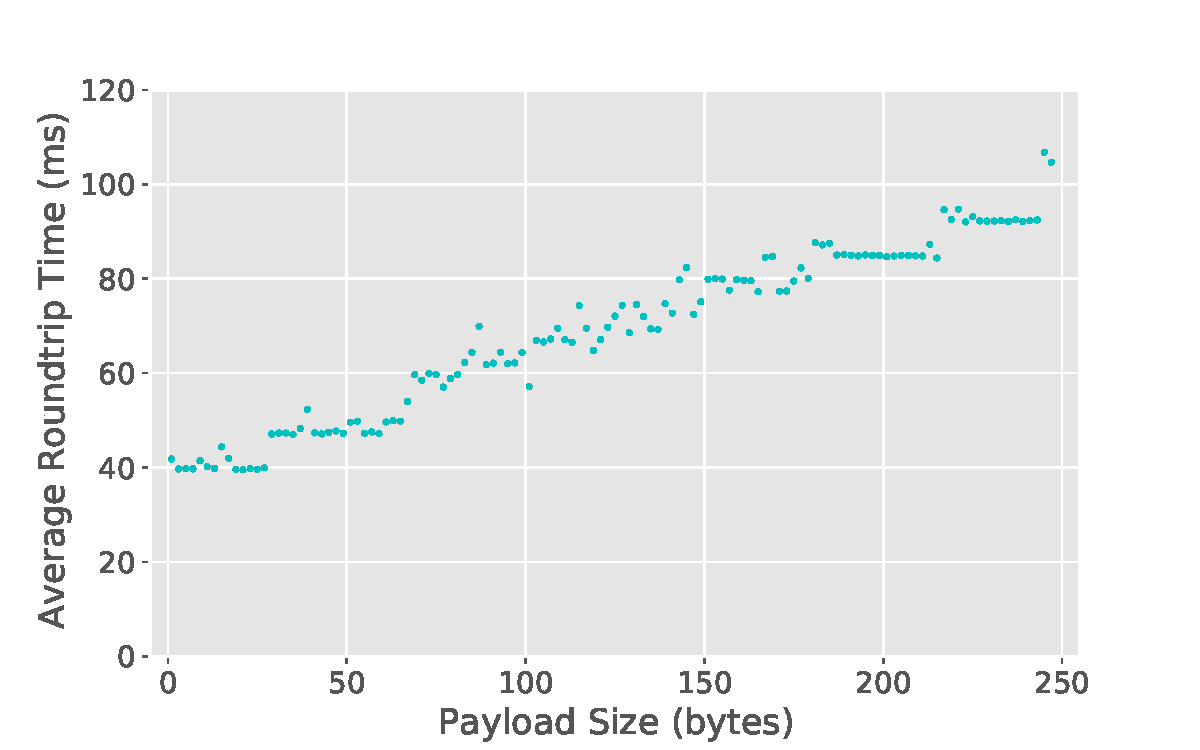
\includegraphics[width=0.75\linewidth]{images/ble-roundtrip-hci0-300cm.pdf}
    \label{fig:ble-roundtrip-hci0-3m}
    \caption[Average \acs{BLE} connection roundtrip time obtained using the Asus USB-BT500 adapter at a distance of 3m.]{Average \acs{BLE} connection roundtrip time obtained using the Asus USB-BT500 adapter at a distance of $3\text{m} \pm 0.2$.}
\end{figure}

\begin{figure}[H]
    \centering
    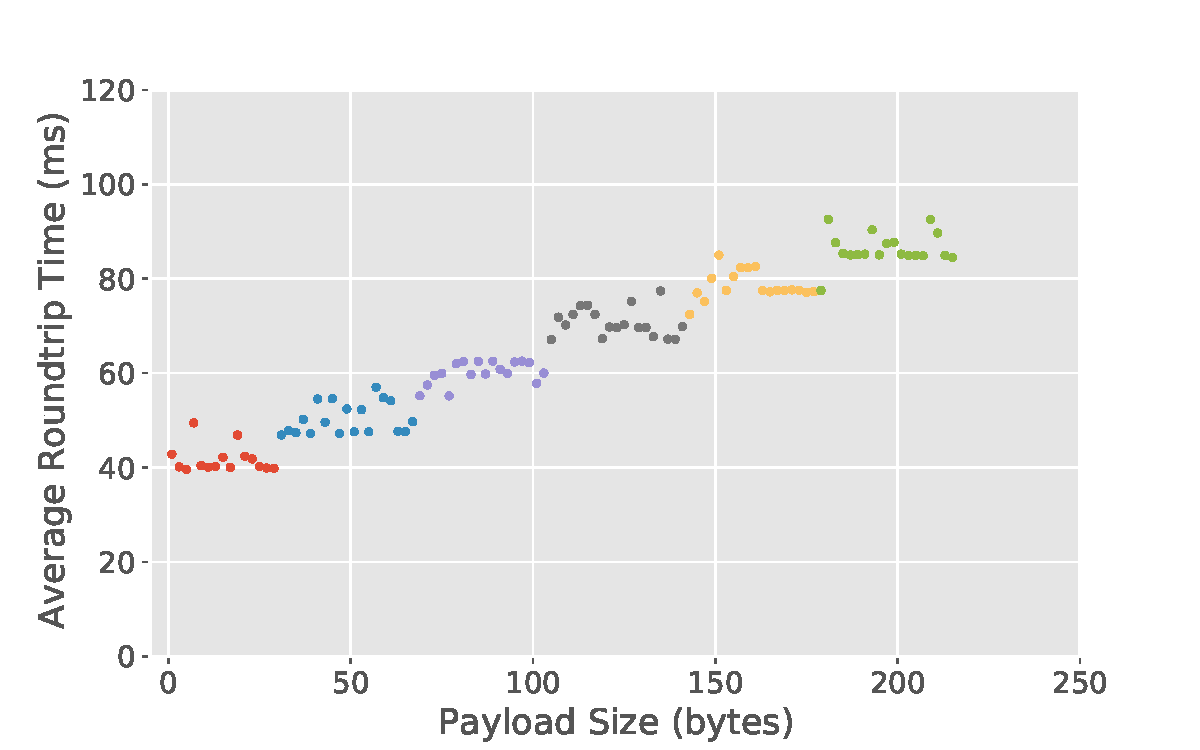
\includegraphics[width=0.75\linewidth]{images/ble-roundtrip-hci0-600cm.pdf}
    \label{fig:ble-roundtrip-hci0-6m}
    \caption[Average \acs{BLE} connection roundtrip time obtained using the Asus USB-BT500 adapter at a distance of 6m.]{Average \acs{BLE} connection roundtrip time obtained using the Asus USB-BT500 adapter at a distance of $6\text{m} \pm 0.2$.}
\end{figure}

\begin{figure}[H]
    \centering
    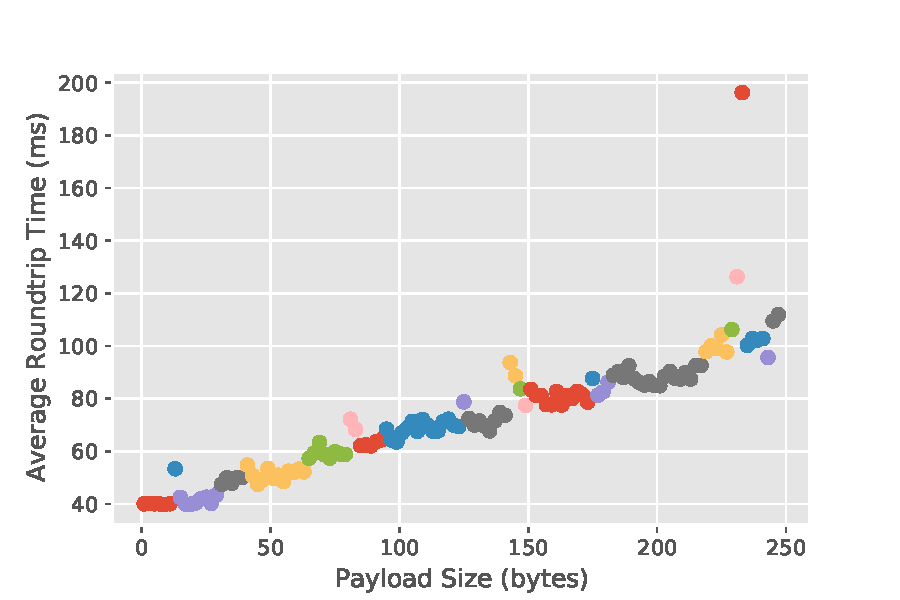
\includegraphics[width=0.75\linewidth]{images/ble-roundtrip-hci0-900cm.pdf}
    \label{fig:ble-roundtrip-hci0-9m}
    \caption[Average \acs{BLE} connection roundtrip time obtained using the Asus USB-BT500 adapter at a distance of 9m.]{Average \acs{BLE} connection roundtrip time obtained using the Asus USB-BT500 adapter at a distance of $9\text{m} \pm 0.2$.}
\end{figure}

We find that for both adapters, the minimum roundtrip time is the same: appoximately ~40ms. This is an odd value, given that the connection interval was set to 7.5ms, meaning the time it takes to transmit a single message and recieve it on the \acs{SmartBox} takes nearly x4 connection intervals, nearly double of what should be expected. Nonetheless, it is still a 
 
We can also observe that for both adapters, the roundtrip times measurements become significantively noisy as the distance increases, as expected, although it is particularly noticable for the Raspberry Pi 4B's internal \acs{BLE} adapter on Figure \ref{fig:ble-roundtrip-hci1-9m}. 

\paragraph{} During the development of these tests, we discovered an functionaly which was not documented in the specification -- \acf{DLE}. This feature, introduced in Bluetooth 4.2, allows \acs{LL} data packet payload to increase significantly in size, up to 251 bytes (compared to the 23 bytes when not using this feature). This gives a lead start for the Asus USB-BT500, as it is capable of sending nearly x10 more data in a single transmission, compared to the Raspberry Pi 4B's internal \acs{BLE} adapter.

\paragraph{} 

\subsubsection{Test 2: Bandwidth Measurement}

In this second test, we measure the maximum bandwidth for the \acs{BLE} connection by adjusting the transmission rate, or more accurately, the time between the transmission of each packet. 

For this test, the nRF52-DK board exposed 7 \acs{GATT} characteristics for the \textit{SmartBox} to subscribe to. The nRF52-DK then continuously changes the value of the characteristic, immediately triggering a notification to the \textit{SmartBox} -- one for each characteristic. The transmission rate was increased until the connection became to unstable and crashed. Below, are the bandwidth graphs obtained for different transmission rates (which correspond to the frequency with which the characteristics are updated) for each adapter. Each test was run 3 times to ensure the results are consistent.


\begin{figure}[H]
    \centering
    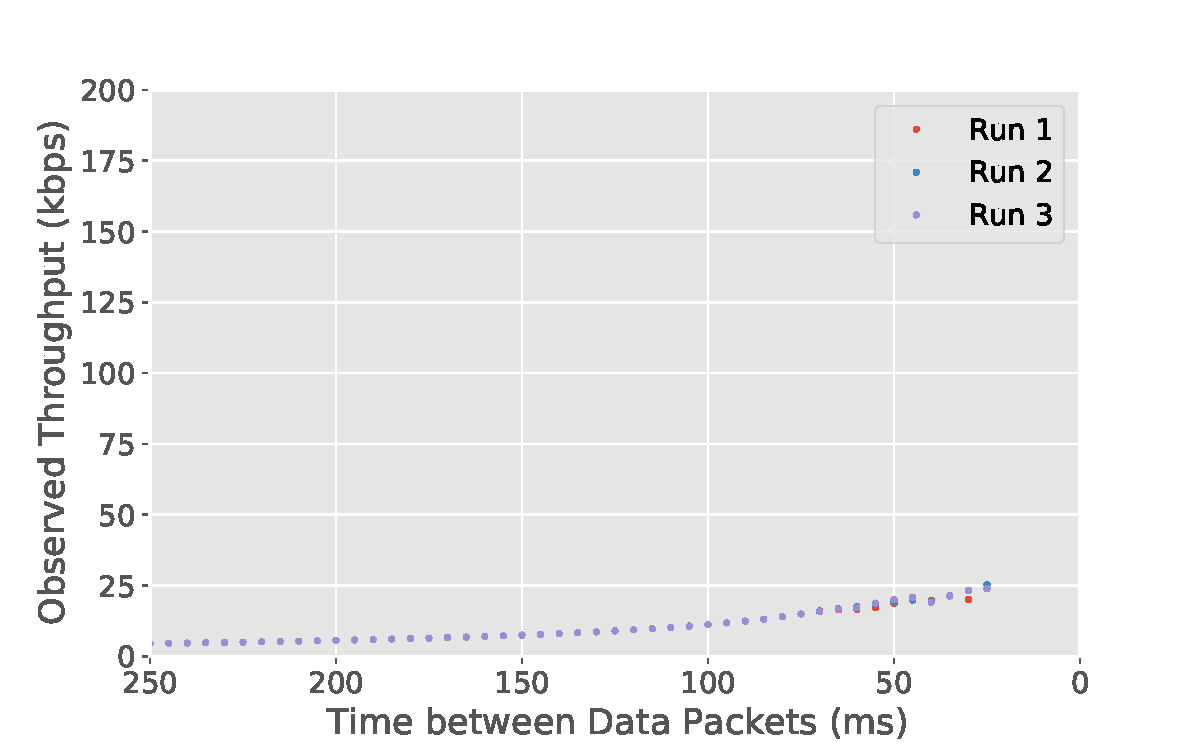
\includegraphics[width=0.75\linewidth]{images/ble-bandwidth-hci1-0cm.pdf}
    \caption[\acs{BLE} connection bandwidth obtained using the Asus USB-BT500 adapter at a distance of 0m.]{\acs{BLE} connection bandwidth obtained using the Raspberry Pi 4B internal \acs{BLE} adapter at a distance of $0\text{m} \pm 0.2$.}
    \label{fig:ble-bandwidth-hci1-0m}
\end{figure}

\begin{figure}[H]
    \centering
    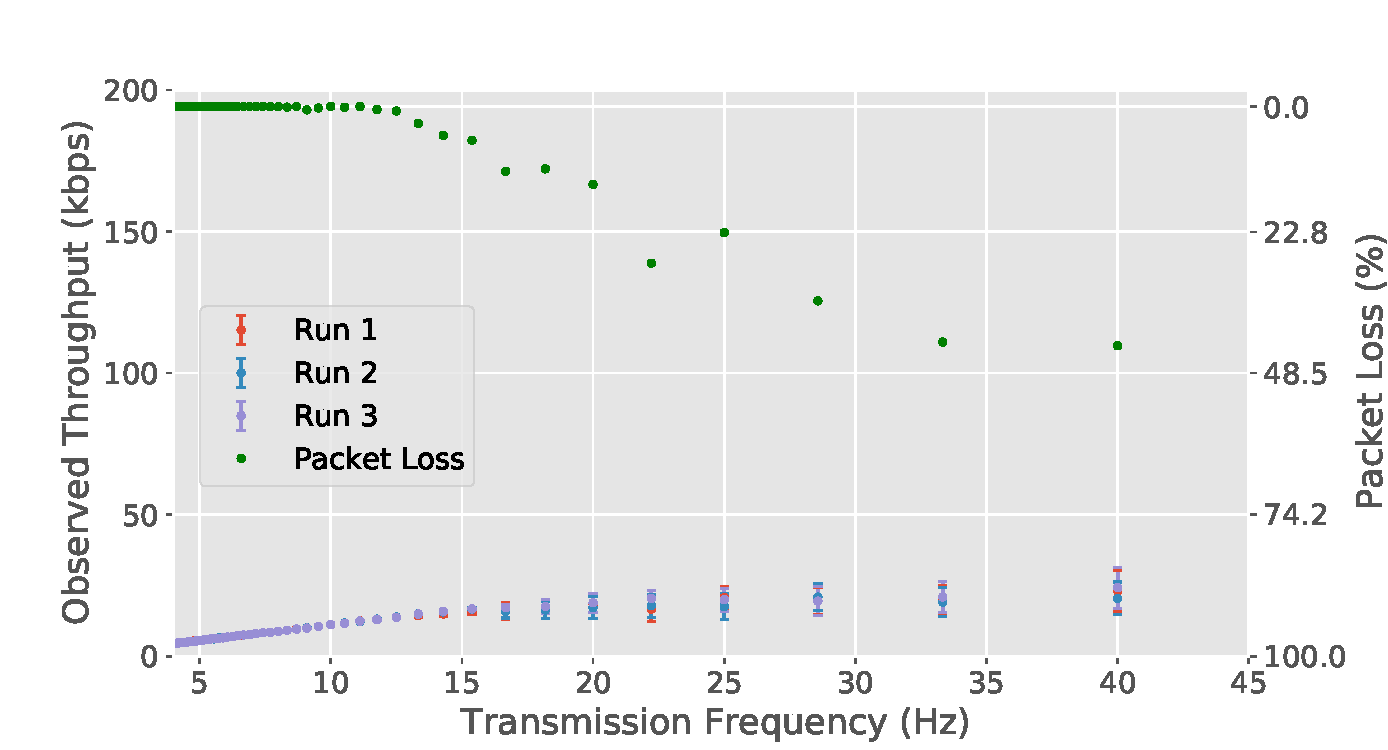
\includegraphics[width=0.75\linewidth]{images/ble-bandwidth-hci1-300cm.pdf}
    \caption[\acs{BLE} connection bandwidth obtained using the Asus USB-BT500 adapter at a distance of 3m.]{\acs{BLE} connection bandwidth obtained using the Raspberry Pi 4B internal \acs{BLE} adapter at a distance of $3\text{m} \pm 0.2$.}
    \label{fig:ble-bandwidth-hci1-3m}
\end{figure}

\begin{figure}[H]
    \centering
    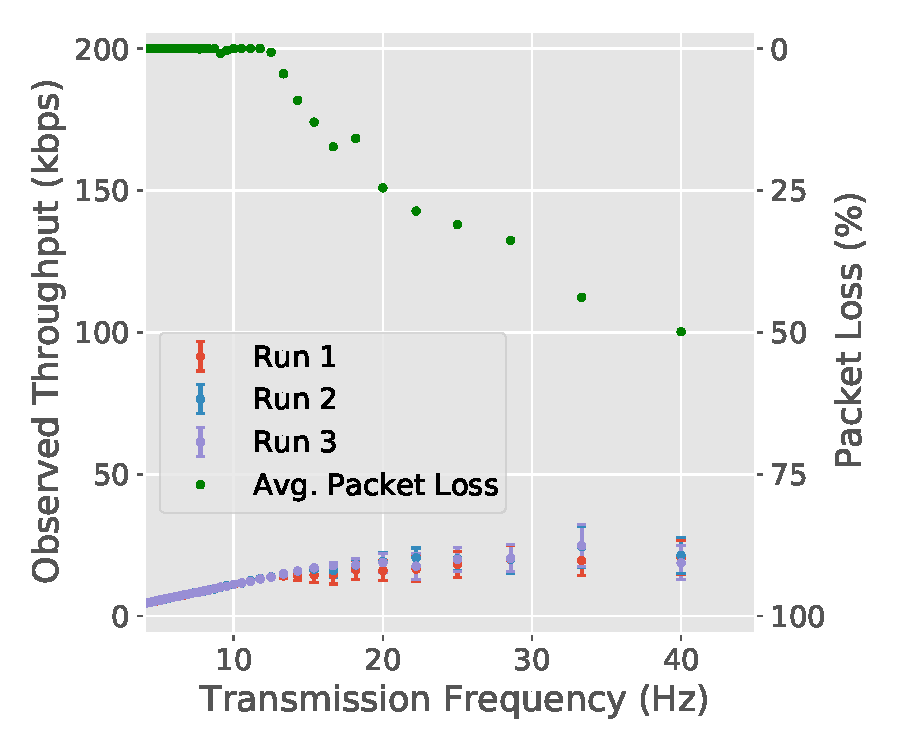
\includegraphics[width=0.75\linewidth]{images/ble-bandwidth-hci1-600cm.pdf}
    \caption[\acs{BLE} connection bandwidth obtained using the Asus USB-BT500 adapter at a distance of 6m.]{\acs{BLE} connection bandwidth obtained using the Raspberry Pi 4B internal \acs{BLE} adapter at a distance of $6\text{m} \pm 0.2$.}
    \label{fig:ble-bandwidth-hci1-6m}
\end{figure}

\begin{figure}[H]
    \centering
    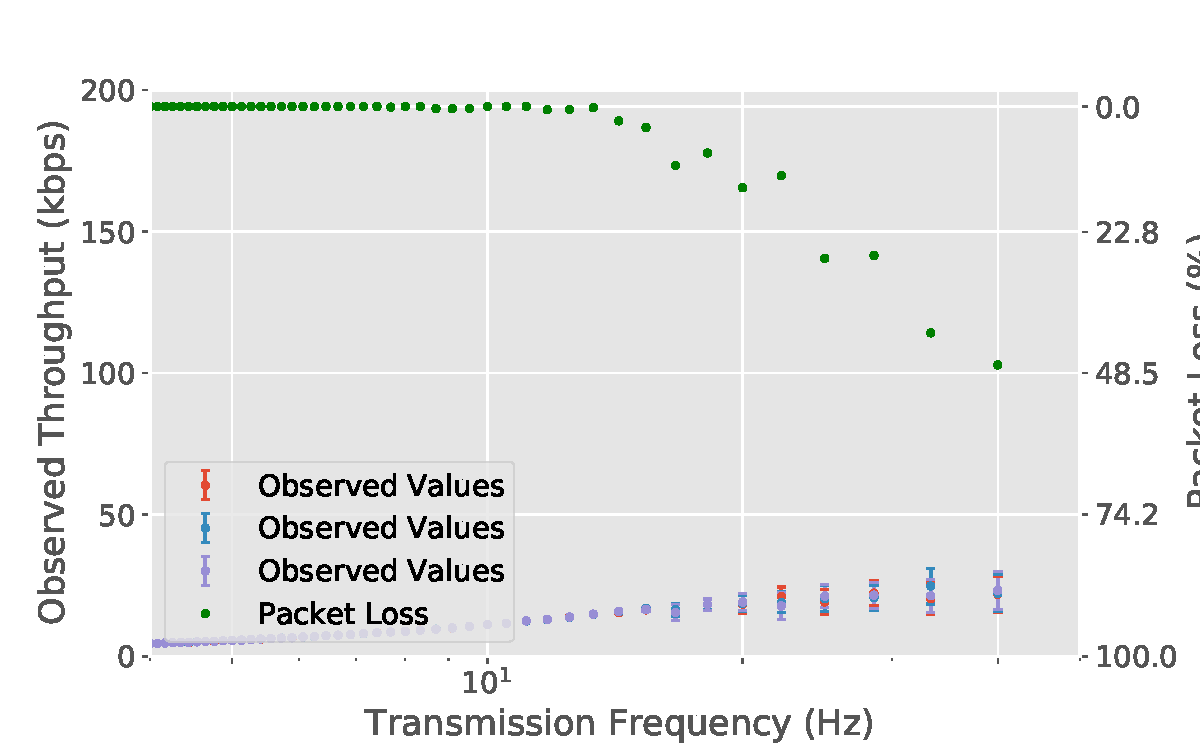
\includegraphics[width=0.75\linewidth]{images/ble-bandwidth-hci1-900cm.pdf}
    \caption[\acs{BLE} connection bandwidth obtained using the Asus USB-BT500 adapter at a distance of 9m.]{\acs{BLE} connection bandwidth obtained using the Raspberry Pi 4B internal \acs{BLE} adapter at a distance of $9\text{m} \pm 0.2$.}
    \label{fig:ble-bandwidth-hci1-9m}
\end{figure}

\begin{figure}[H]
    \centering
    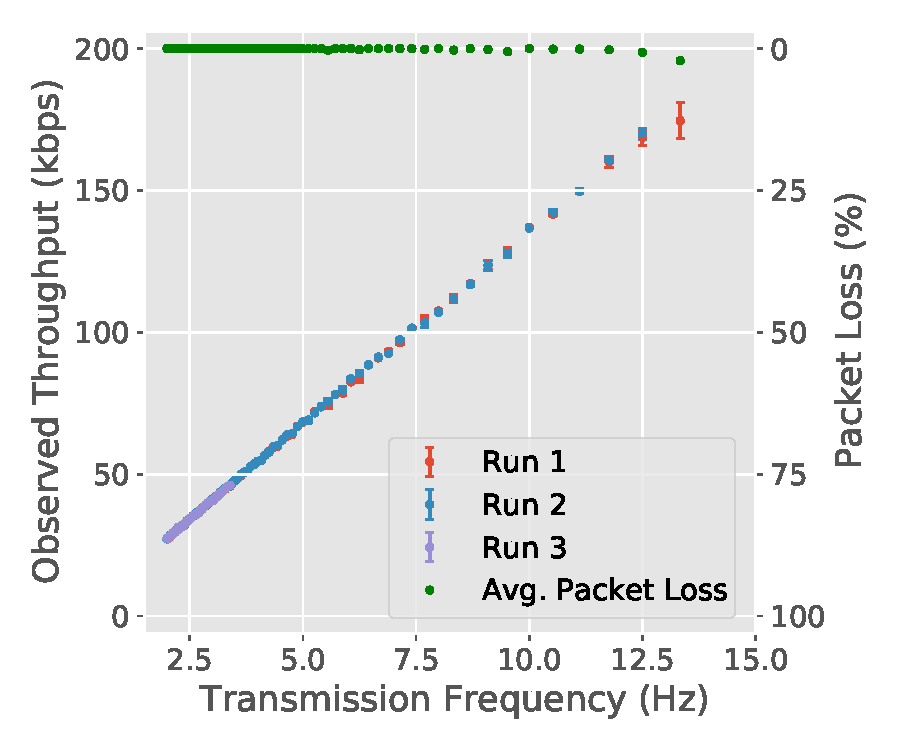
\includegraphics[width=0.75\linewidth]{images/ble-bandwidth-hci0-0cm.pdf}
    \caption[\acs{BLE} connection bandwidth obtained using the Asus USB-BT500 adapter at a distance of 0m.]{\acs{BLE} connection bandwidth obtained using the Asus USB-BT500 adapter at a distance of $0\text{m} \pm 0.2$.}
    \label{fig:ble-bandwidth-hci0-0m}
\end{figure}

\begin{figure}[H]
    \centering
    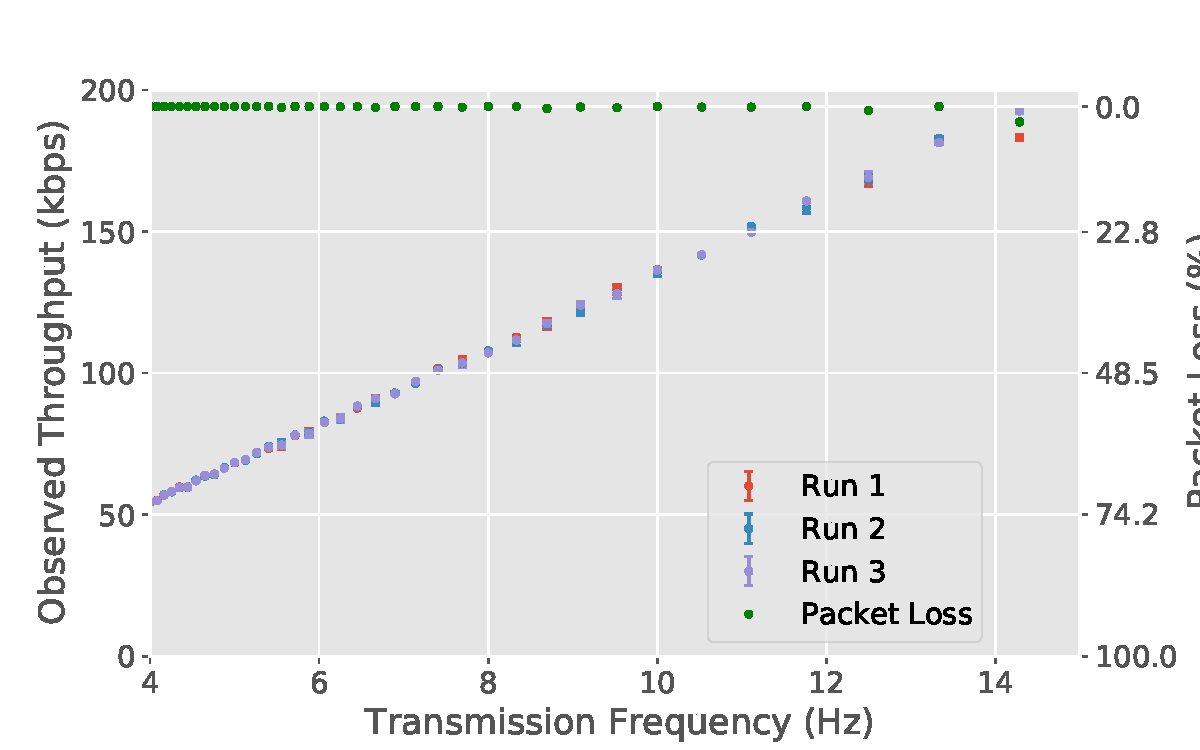
\includegraphics[width=0.75\linewidth]{images/ble-bandwidth-hci0-300cm.pdf}
    \caption[\acs{BLE} connection bandwidth obtained using the Asus USB-BT500 adapter at a distance of 3m.]{\acs{BLE} connection bandwidth obtained using the Asus USB-BT500 adapter at a distance of $3\text{m} \pm 0.2$.}
    \label{fig:ble-bandwidth-hci0-3m}
\end{figure}

\begin{figure}[H]
    \centering
    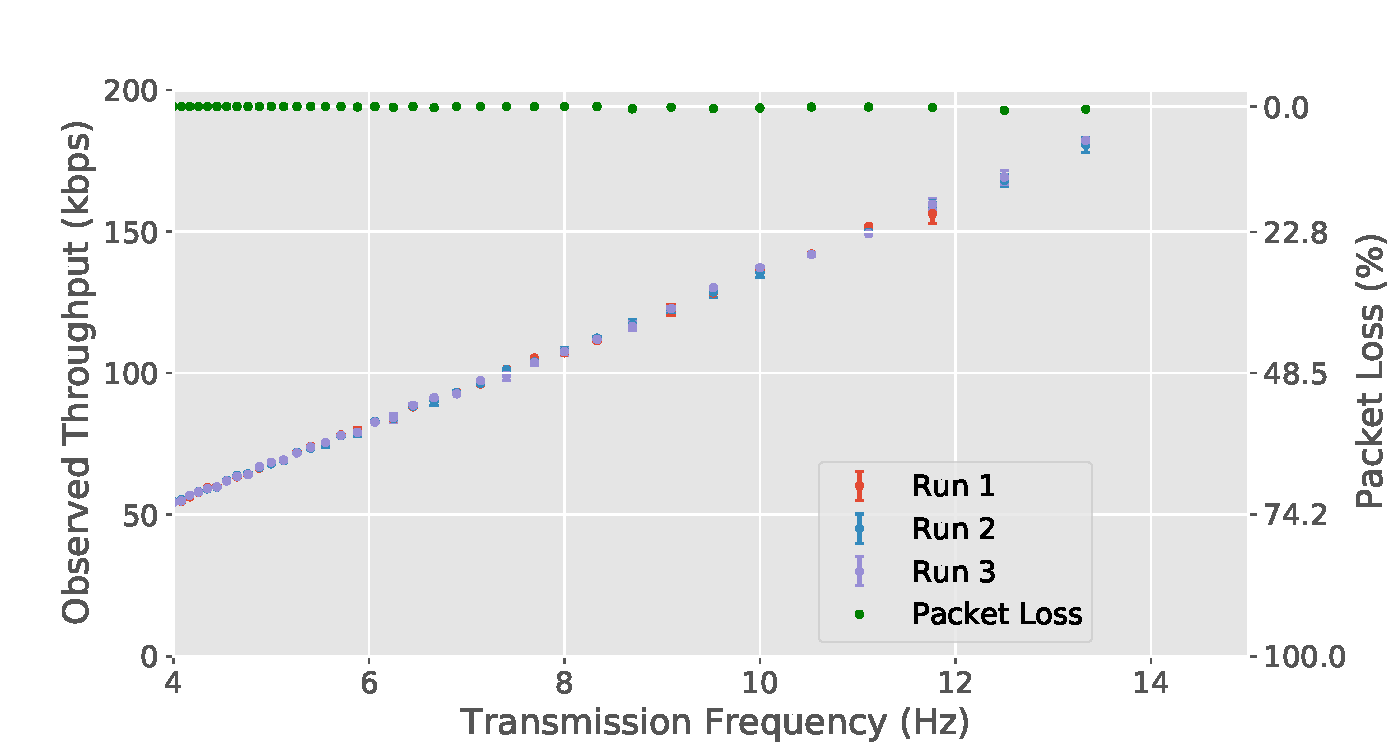
\includegraphics[width=0.75\linewidth]{images/ble-bandwidth-hci0-600cm.pdf}
    \caption[\acs{BLE} connection bandwidth obtained using the Asus USB-BT500 adapter at a distance of 6m.]{\acs{BLE} connection bandwidth obtained using the Asus USB-BT500 adapter at a distance of $6\text{m} \pm 0.2$.}
    \label{fig:ble-bandwidth-hci0-6m}
\end{figure}

\begin{figure}[H]
    \centering
    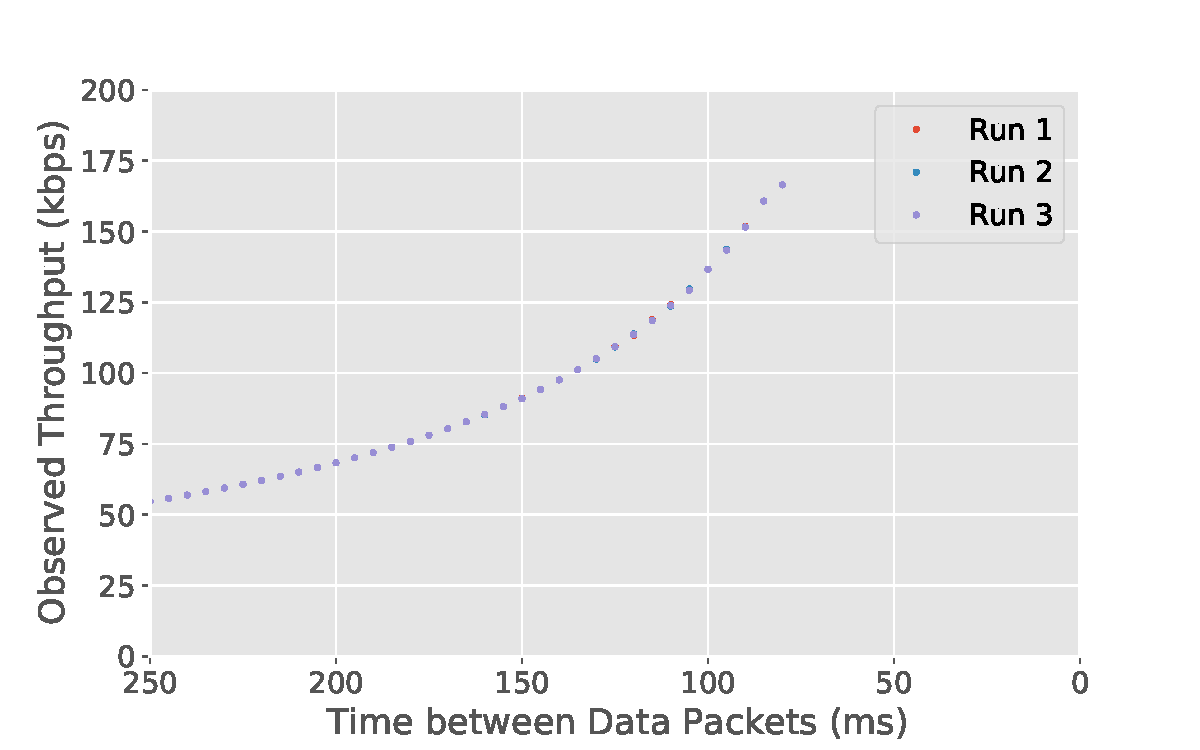
\includegraphics[width=0.75\linewidth]{images/ble-bandwidth-hci0-900cm.pdf}
    \caption[\acs{BLE} connection bandwidth obtained using the Asus USB-BT500 adapter at a distance of 9m.]{\acs{BLE} connection bandwidth obtained using the Asus USB-BT500 adapter at a distance of $9\text{m} \pm 0.2$.}
    \label{fig:ble-bandwidth-hci0-9m}
\end{figure}



\subsection{Decision on \acs{BLE} adapter}

From the previous tests, we see that the internal \acs{BLE} adapter lacks the support for \acs{DLE} feature, which reduces greatly the communication throughput.  



\section{Summary}
In this chapter, we \dots

\chapter{Smart Gateway Development}
\label{chap:gateway}


In the proposed architecture, the \textit{Smart Gateway} is the central module of the system, connecting the \textit{SmartBoxes} to the \acs{HIS}. It is responsible for the management of devices and their associations -- \textit{SmartBox} to \textit{Biosticker} and \textit{SmartBox} to user -- managing, maintaining and storing the data that is generated by these, as well as handling any communication to and from the \acs{HIS}. 


\paragraph{} Regarding the hardware platform used to implement the \textit{Smart Gateway}, in context of the \acs{WoW} project, we use the Intel NUC NUC8i7BEH\footnote{\url{https://ark.intel.com/content/www/br/pt/ark/products/126140/intel-nuc-kit-nuc8i7beh.html}}.

\begin{figure}[H]
    \centering
    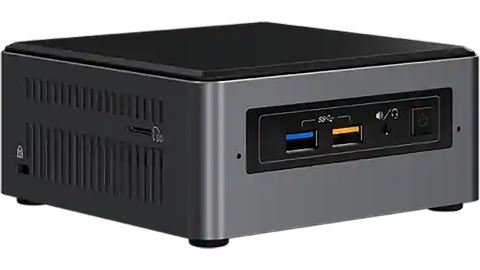
\includegraphics[width=0.5\linewidth]{images/gateway-image.png}
    \caption[Intel NUC NUC8i7BEH.]{Intel NUC NUC8i7BEH.}
    \label{fig:gateway_image}
\end{figure}


\paragraph{} In the next sections, we propose a service architecture for the \textit{Smart Gateway} in order to fulfill the aforementioned features.

% The \textit{Smart Gateway} maintains a list of all the \textit{SmartBoxes} that are managed by the system, as well as every \textit{Biosticker} and every sensor in the \textit{Biosticker} (which are used to indicate respective biosignal to the \acs{HIS}). 


\section{Service Architecture}

The \textit{Smart Gateway} must..

\begin{itemize}
    \item Manage devices and device associations: The \textit{Smart Gateway} maintains a list of all the \textit{SmartBoxes} that are managed by the system, as well as every \textit{Biosticker} and every sensor in the \textit{Biosticker} (which are used to indicate respective biosignal to the \acs{HIS}). 
    \item Data anonymization;
    \item Data pre-processing;
    \item Real-time data collection;
    \item 
\end{itemize}

\paragraph{} Figure \ref{fig:gateway_serviceoverview} illustrates the different services implemented in the \textit{Smart Gateway}.

\begin{figure}[H]
    \centering
    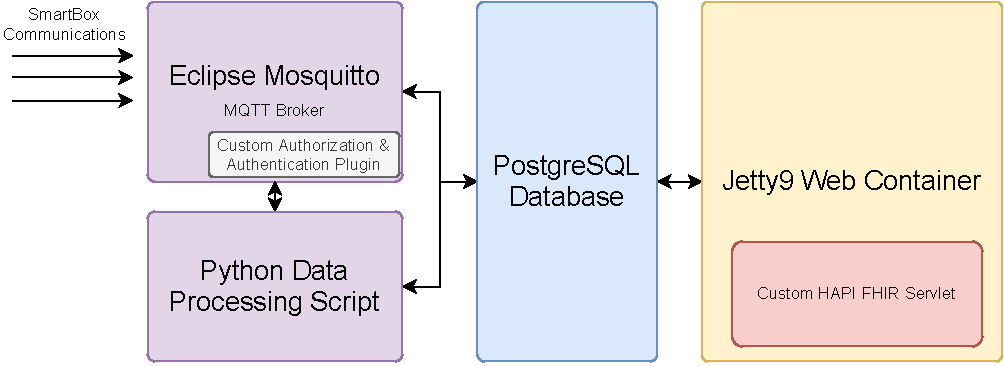
\includegraphics[width=\linewidth]{images/service overview gateway.pdf}
    \caption[Service architecture implemented in the \textit{Smart Gateway}.]{Service architecture implemented in the \textit{Smart Gateway}. The diagram displays the different technologies used throughout the development. The services communicate with each other using Unix Sockets, a Linux exclusive protocol for \acf{IPC}.}
    \label{fig:gateway_serviceoverview}
\end{figure}


\subsection{Security on Linux}
- o isolamento dos processos é feito através do "utilizador" que está a executar o processo. cada processo tem apenas acesso aos seus serviços.

- indicar que estamos a usar Unix Sockets para a comunicação entre processos;

- o uso de unix sockets permite usar o sistema de permissões do sistema operativo para controlar o acesso às sockets (através dos ``utilizadores'' que estão a executar os serviços).

\paragraph{} As seen above, these services have 

\section{Data Storage}

The data storage in the \textit{Smart Gateway} is one of the most important components of the device, as it holds the information used by all services in the \textit{Smart Gateway}. Given the importance of this component, it is crucial to use a solution which offers reliability above all with great performance for our use case.  

\paragraph{} As discussed in Section \ref{sec:iot-model-layer4}, No\acs{SQL} databases are appealing for \acs{IoT} applications, since these have great performance..

% it is important to choose a solution which offers availability

% PostgreSQL offers a balance between \footnote{\url{https://itnext.io/benchmark-databases-in-docker-mysql-postgresql-sql-server-7b129368eed7?gi=a506815fb197}}

\subsection{Database Schema}
Figure \ref{fig:wow-dbschema-full} contains the database model implemented in our PostgreSQL database. It describes all information that is contained in the \textit{Smart Gateway}, the relations within that data, organized according to the functionality it is related to, which will be explored in greater detail in the next sections.


\begin{figure}[H]
    \centering
    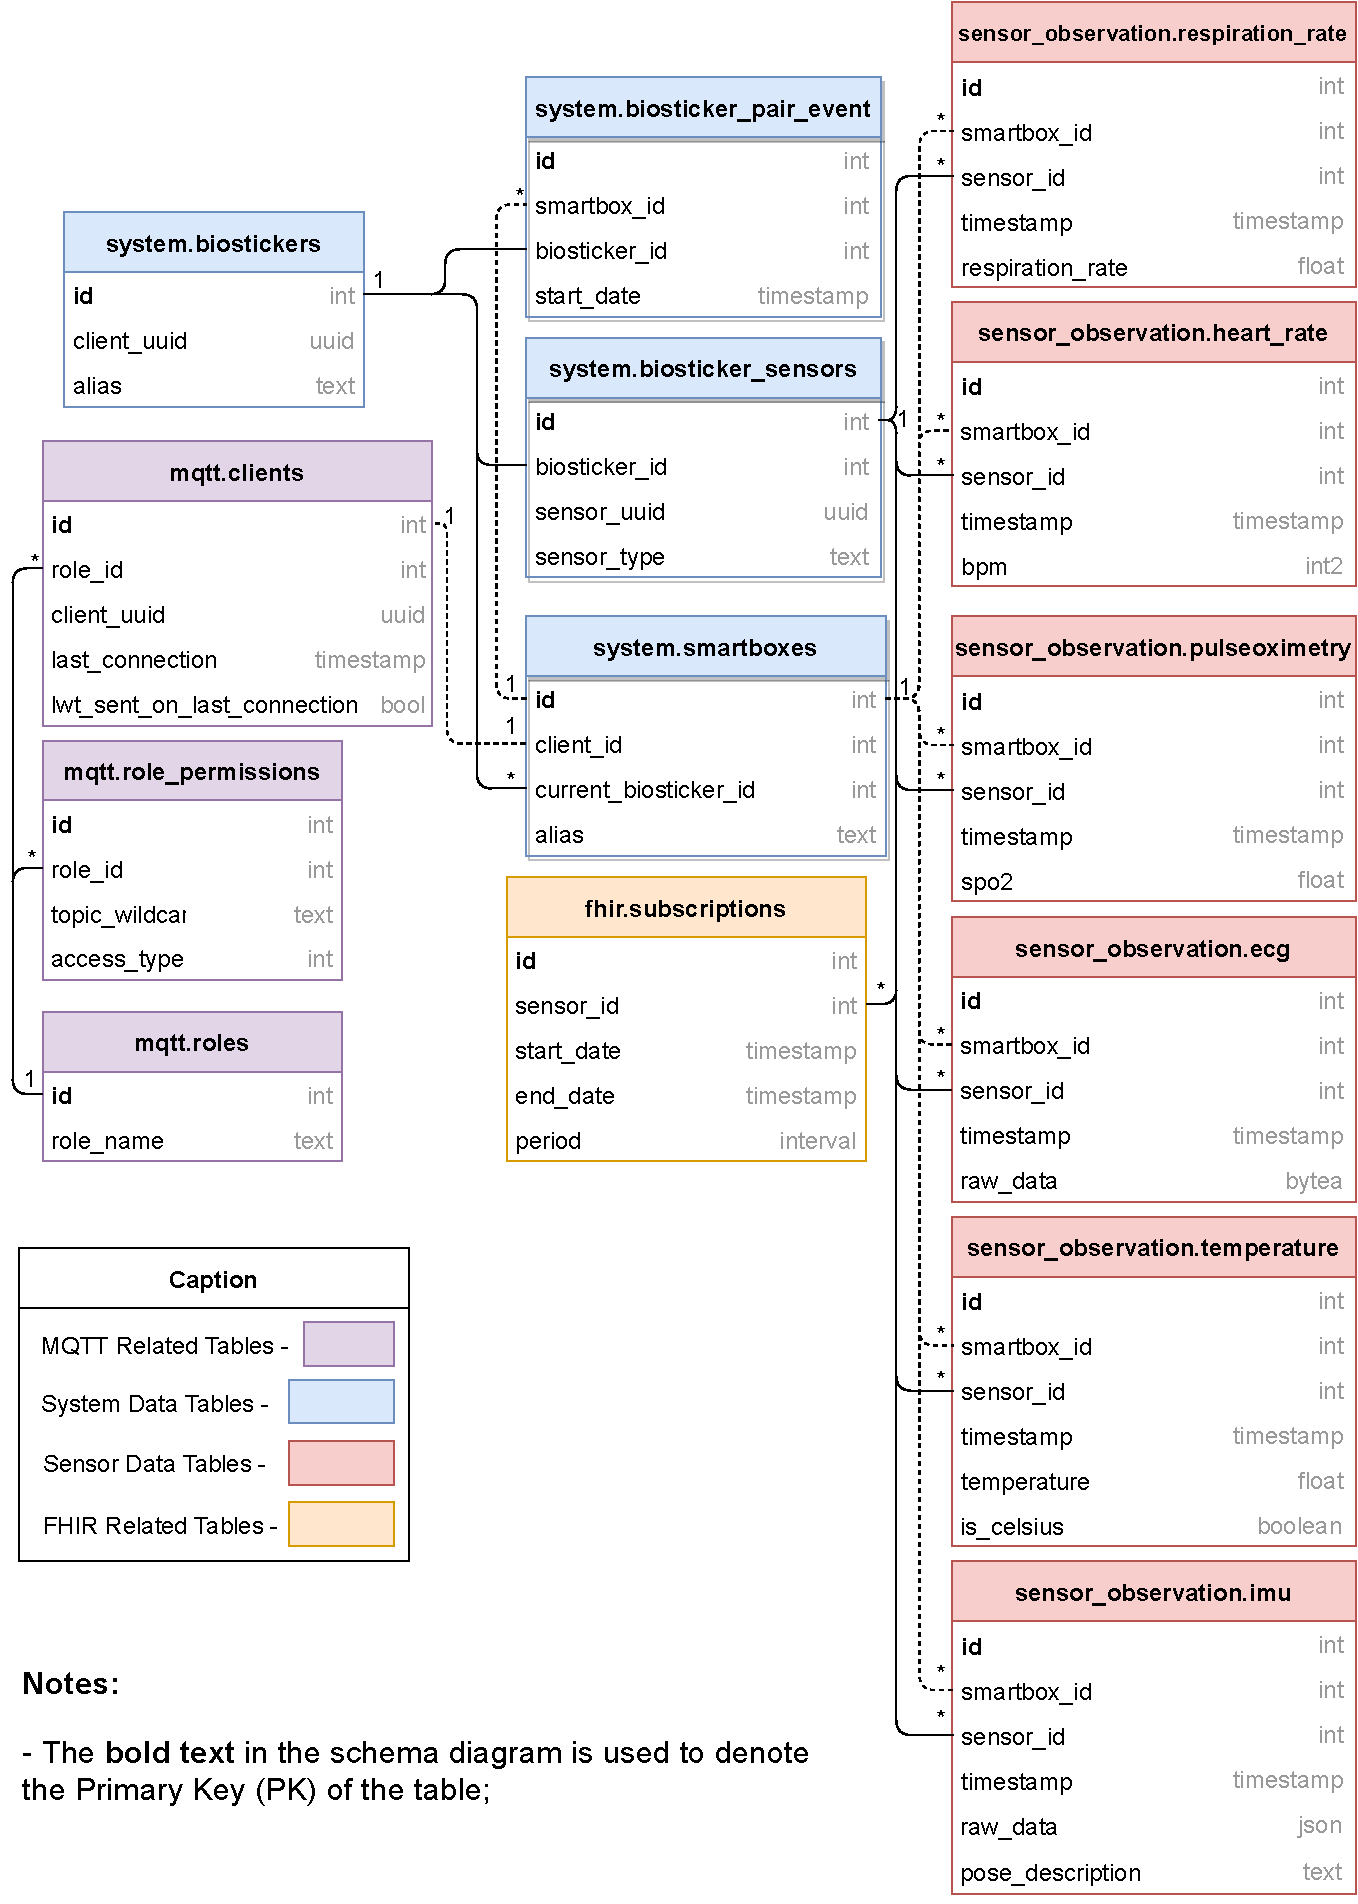
\includegraphics[width=0.86\linewidth]{images/database-schema-general.pdf}
    \caption[Database schema implemented in the \textit{Smart Gateway}.]{Database schema implemented in the \textit{Smart Gateway}.}
    \label{fig:wow-dbschema-full}
\end{figure}

\subsubsection{MQTT Client Information}

Figure \ref{fig:wow-dbschema-mqtt} contains the information relevant for \acs{MQTT} communications, mostly related with security. To ensure that each device only has access to its own resources, the system implements a \acf{RBAC} policy. 
In this type of access control, the system allows and revokes access to resources according to the role of the device. 

\paragraph{} In context of the \acs{WoW} project, the following roles are used:

\begin{itemize}
    \item \textit{SmartBox} role: Indicates the \acs{MQTT} client is a \textit{SmartBox}.
    \item ``Pyservice'' role: Indicates the \acs{MQTT} client is actually the data processing service, also contained in the \textit{Smart Gateway}.
    \item Developer device role: Indicates the \acs{MQTT} client is a developer device, used solely for debugging purposes.
\end{itemize}


\begin{figure}[H]
    \centering
    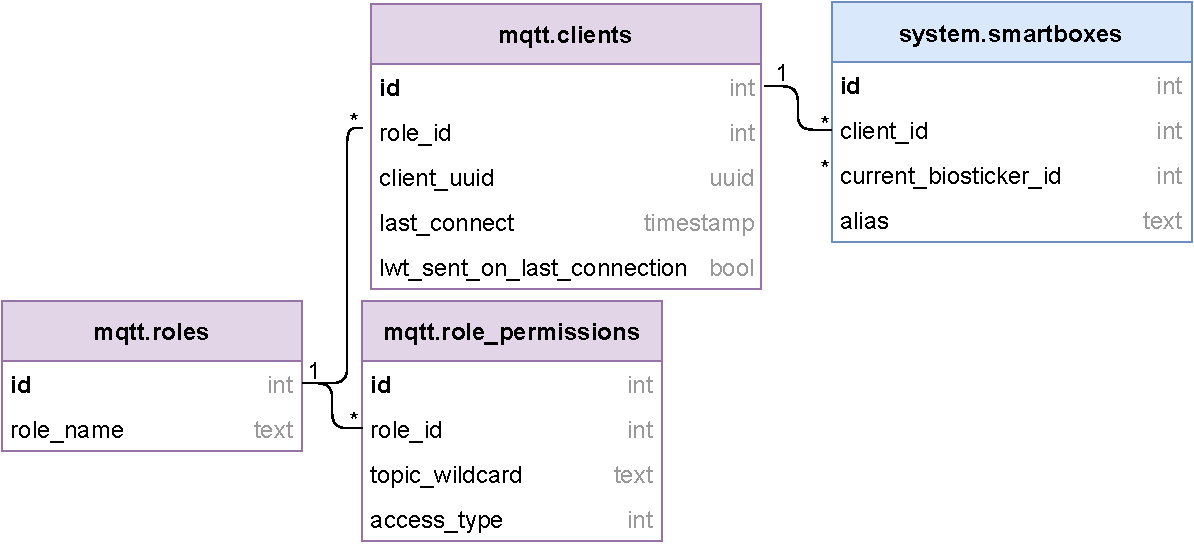
\includegraphics[width=\linewidth]{images/database-schema-mqtt.pdf}
    \caption[\acs{MQTT} information in the schema implemented in the \textit{Smart Gateway}.]{\acs{MQTT} information in the schema implemented in the \textit{Smart Gateway}.
    The ``mqtt.roles'' table contains the different \acs{RBAC} roles for the \acs{MQTT} communication and ``mqtt.role\_permissions'' table lists the permissions available to each role using \acs{MQTT} topic wildcards. The ``mqtt.client'' table lists the clients and their properties, such as their \acs{UUID}, the timestamp of their last connection, or a \textit{flag} to indicate if the communication failed during the last communication.
    
    }
    \label{fig:wow-dbschema-mqtt}
\end{figure}

\subsubsection{Sensor Data}

Figure \ref{fig:wow-dbschema-sensors} contains the sensor data collected over time. The tables 

\begin{figure}[H]
    \centering
    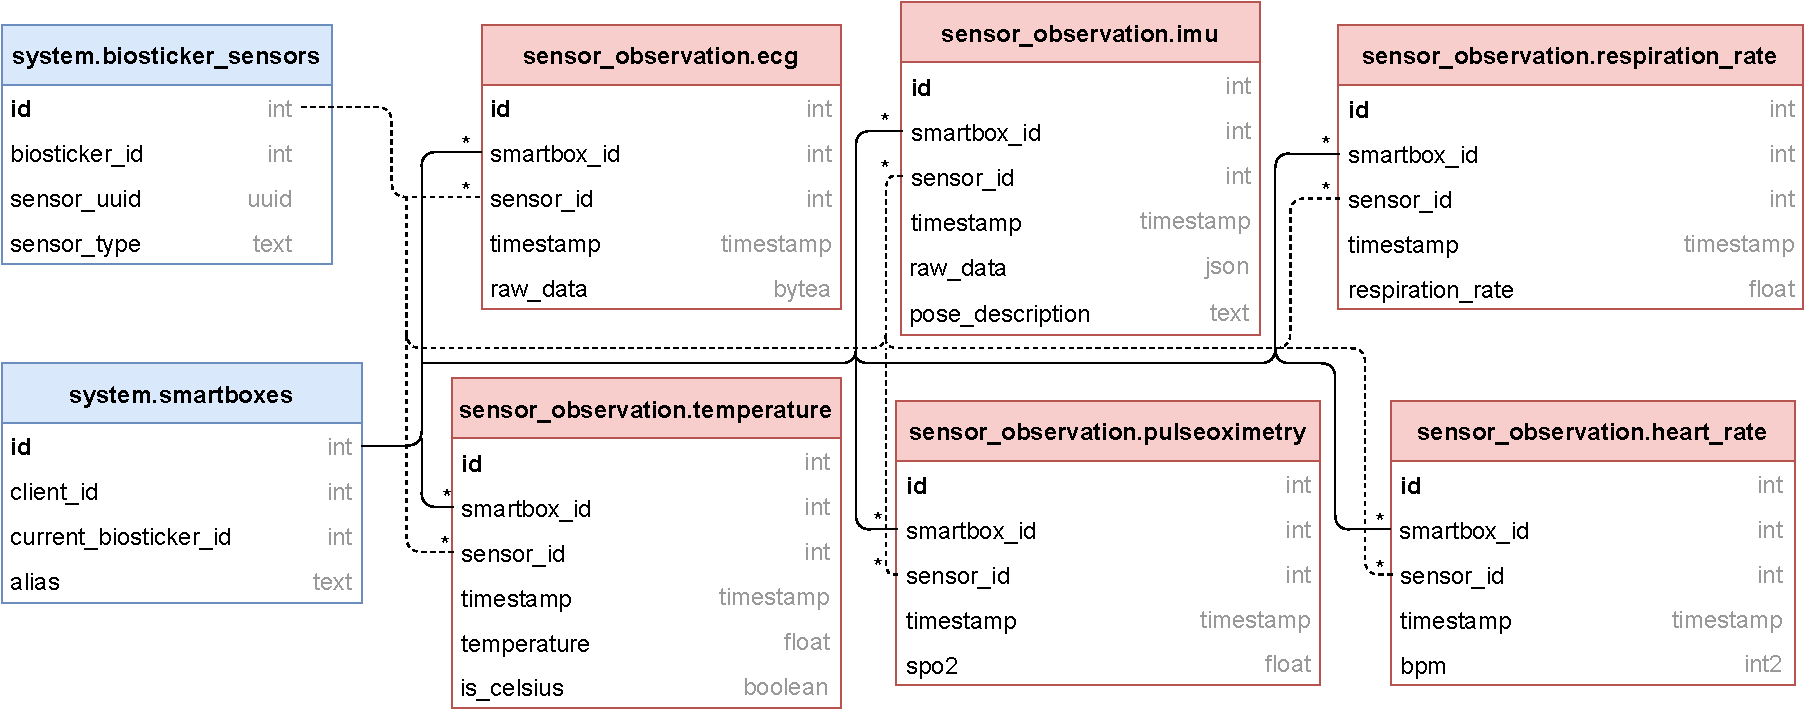
\includegraphics[width=\linewidth]{images/database-schema-sensordata.pdf}
    \caption[Sensor data information in the schema implemented in the \textit{Smart Gateway}.]{
        Sensor data information in the schema implemented in the \textit{Smart Gateway}. Our database model has one table for each different type of biosignal (temperature, \acs{ECG}, etc.). The properties of the table are defined according to the data acquired on the \textit{SmartBox} level, which are detailed in Section \ref{sec:biosticker_data}.}
    \label{fig:wow-dbschema-sensors}
\end{figure}

\subsubsection{FHIR Related Information}
\dots 

\begin{figure}[H]
    \centering
    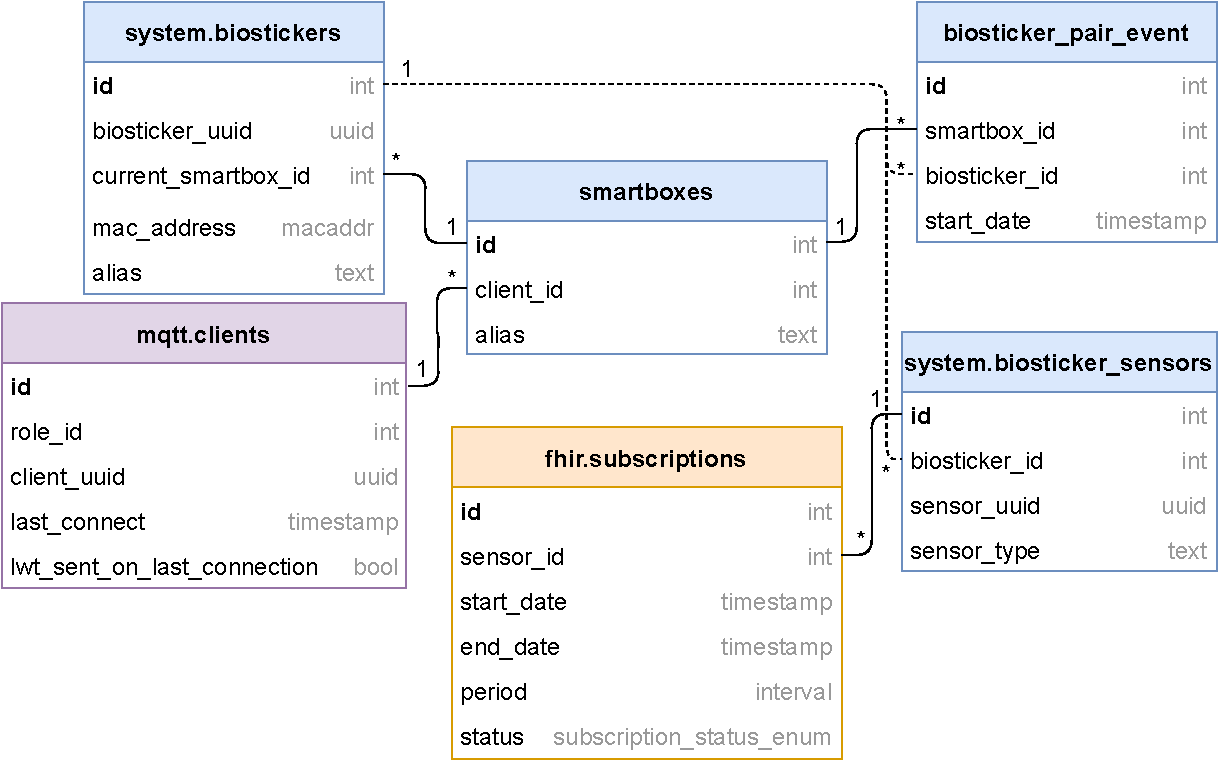
\includegraphics[width=\linewidth]{images/database-schema-fhir.pdf}
    \caption[test]{test}
    \label{fig:wow-dbschema-fhir}
\end{figure}
 

\subsubsection{Stored Procedures}

%During development, we noticed that our database service was consuming a concerning amount of resources when 
- de modo a maximizar o desempenho do serviço da base de dados, os diferentes pedidos de base de dados (queries) foram configurados e pré-compilados na base de dados. isto reduz o tamanho dos pedidos enviados à base de dados (pois em vez de enviar transações complexas, executamos apenas uma função na base de dados), faz com que a base de dados não tenha de validar a estrutura dos pedidos (porque já foi pre-compilada), particularmente para eviar injeções de SQL.

\section{Connection to the SmartBoxes}

As previously mentioned, the connection to the \textit{SmartBoxes} is performed via \acs{MQTT}. \acs{MQTT} is a centralized protocol, in which the clients (\textit{SmartBoxes}) connect to a broker, which acts as a middle-man for the communication, managing the requests from all clients accordingly. In our system, the broker is contained within the \textit{Smart Gateway}, and is the service responsible for ensuring the communication between the \textit{SmartBoxes} and our \acs{IoT} system.

\paragraph{} To implement this \acs{MQTT} broker, we use the open-source Eclipse Mosquitto\footnote{Eclipse Mosquitto -- An open-source \acs{MQTT} broker: \url{https://mosquitto.org/}}. Mosquitto is a lightweight \acs{MQTT} broker that supports the \acs{MQTT} protocol versions 5.0, 3.1.1 and 3.1 and is widely used by the community, making it a fitting solution for the \acs{WoW} project.

\paragraph{} One of the 



It is extremely flexible since it allows developers to extend its functionality using plugins

exposes an \acs{API}

extensible 

\paragraph{} 


\subsection{Specification for \acs{MQTT} Communication}
- indicar que foi proposta uma especificação para a comunicação MQTT

\subsection{Authorization and Authentication Plugin}
- 
- a segurança no MQTT é feita através de 2 points
- a segurança no mosquitto atualmente é feita através de um ficheiro estático (lol) que define as permissões dos clientes que acedem o servidor.
- de modo a assegurar 

\section{Integration with GlobalCare}

- Mini introdução ao FHIR;
- mencionar camada de interoperabilidade da globalcare;
- indicar que optou-se usar HAPI devido ao facto de ser uma iniciativa open-source suportada por uma empresa de software hospitalar de renome.
- HAPI FHIR é baseada em Java servlets, fazer mini introdução do que são servlets e explicar o porquê de usar Jetty para correr servlets (é um web container, cujo objetivo é correr servlets). 

\subsection{FHIR Server}

- Falar do que são os FHIR Resources, e mais especificamente dos Resources usados para transmitir os dados -> Bundle, Device, Observation
- Apresentação do diagrama de comunicação de informação

\section{Summary}

In this chapter, we presented the different components which form the \textit{Smart Gateway}. In the chapter, we evaluate the performance of our proposed solution through a hospital trial.

\chapter{Results and Discussion}
\label{chap:results}

\section{Hospital Pilot}


\begin{figure}[H]
    \centering
    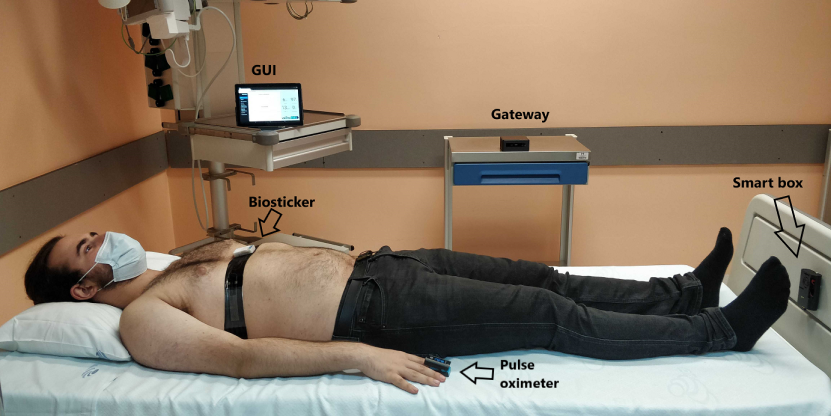
\includegraphics[width=\linewidth]{images/hospital-trial.png}
    \caption[Conceptual illustration of the system components within a medical facility.]{Conceptual illustration of the system components within a medical facility.}
    \label{fig:hospital-trial}
\end{figure}

\section{Results}

\section{Summary}
In this chapter, we \dots

\chapter{Conclusion}
\label{chap:conclusion}
\dots
\section{Future Work}
\dots



% REFERENCES
% Edit the references.bib file to add your own references, that you can then
% \cite on your text.
\bibliographystyle{IEEEtran}
\bibliography{references}

%\titleformat{\chapter}[display]	% Return chapter titles to normal, taking up a whole page (cool for appendices)
%{\normalfont\huge\bfseries}{\chaptertitlename\ \thechapter}{20pt}{\Huge}
%\begin{appendix}			% Start appendices
%\chapter{My cool appendix!}	% One chapter per appendix
%\label{app:cool}
%\includepdf[pages={-}]{path/to/appendix.pdf}
% or
%\input{appendix_file}
%\end{appendix}
\end{document}
